\documentclass[12pt]{book}
\usepackage{amsmath, amssymb, amsthm}
\usepackage{latexsym, epsfig, ulem, cancel, multicol, hyperref}
\usepackage{graphicx, tikz, subfigure,pgfplots}
\usepackage{blindtext}
\usepackage[a4paper, total={6in, 8in}]{geometry}
\setlength{\parindent}{0pt}
\usepackage{multirow}
\usepackage{mathtools}
\usepackage{authblk}
\usepackage{moresize}
\usepackage{makecell}
\pgfplotsset{width=10cm,compat=1.9}
\setlength{\parskip}{1ex}

\title{\textbf{Theory of Relativity Notebook}}
\author[$\dagger$]{
Dennis Li 
\thanks{Special thanks to \textit{Junyao Xu}}
}
\author[$\dagger$]{
Manu Dorghabekov 
}
\affil[$\dagger$]{Prof. Gabriel Perez-Giz}



\newcommand{\liminfty}[1]{\lim_{#1 \to \infty}}
\newcommand{\limzero}[1]{\lim_{#1 \to 0}}
\newcommand{\Z}{\mathbb{Z}}
\newcommand{\R}{\mathbb{R}}
\newcommand{\C}{\mathbb{C}}
\newcommand{\lineint}[1]{\int_{#1}}
\newcommand{\pypx}[2]{\frac{\partial #1}{\partial #2}}
\newcommand{\divg}{\nabla \cdot}
\newcommand{\curl}{\nabla \times}
\newcommand{\dydx}[2]{\frac{\text{d} #1}{\text{d} #2}}
\newcommand{\sqbkt}[1]{\left[ #1 \right]}
\newcommand{\paren}[1]{\left( #1 \right)}
\newcommand{\tribkt}[1]{\left< #1 \right>}
\newcommand{\abso}[1]{\left|#1 \right|}
\newcommand{\bm}[1]{\boldsymbol{#1}}
\newcommand{\etensor}[3]{#1_{#3}^{#2}}
\newcommand{\minkow}{\eta_{\mu\nu}}


\begin{document}

\maketitle
\tableofcontents
\part{Special Relativity}
\chapter{Spacetime - Taylor and Wheeler}
\section{Invariance of Spacetime Interval}

\subsection{Invariance of distance across methods of measurements}

Now let us consider a line segment in the xy-plane as follows
\begin{center}
\begin{tikzpicture}
\begin{axis}
\addplot[color=red]{x};
\end{axis}
\end{tikzpicture}
\end{center}

We can see that the line segment can be the hypotenuse of infinitely many right triangle, whole remaining the same length.\\
and this relationship satisfies the Pythagoras theorem:
\begin{align}
a^2+b^2=c^2
\end{align}
Where $a$ and $b$ are the 2 sides of the right triangle, and $c$ is the hypotenuse.\\
Experimental results shows that there is a similar relationship between space and time.\\
Now we define a similar relationship, instead of on xy-plane, on a space-time plot, as shown below. 
\begin{center}
\begin{tikzpicture}
\begin{axis}[
xmin=-4,
xmax=4,
ymin=-4,
ymax=4,
axis lines=middle,
xlabel=distance,
ylabel=time,
]
\addplot[color=red,domain=-2:2]{x};
\end{axis}
\end{tikzpicture}
\end{center}
Here, we have a space-time plot. And the relationship is not Pythagorean. With experimental results, we find the this line segment follows a relationship such that
\begin{align}
\Delta s^2=-\Delta t^2 + \Delta r^2
\end{align}
Where $\Delta s$ is the space-time interval and $\Delta t$ is the time interval, measured in meters, and $\Delta r$ is the spatial separation.\\
To make sense of this, we have to introduce more context.
\subsection{meters of time, event, spacetime interval}
Let us first get familiar with the concept of \textbf{Event.}\\\\
An \textbf{Event} is basically something that just happens, regardless of who is checking it out. An observer that is interested in a certain series of event (say, 2) could measure the following parameters. 
\begin{enumerate}
    \item The time separation between event 1 and event 2
    \item The spatial separation between event 1 and event 2
\end{enumerate}
One might be tempted to just use these measurements and tryout this relationship of spacetime interval, but there are more works to do before throwing in numbers. We would first have to unify the units of space and time such that the operation make sense.\\
\newline
We start with measuring time in meters, which is not conventional, yet familiar. As we often measures distance with time such as \textit{10 minutes away from school}. We would assume an underlying speed given the means of transportation. And for our purpose, the underlying speed is the speed of light $c$.\\
Therefore, the time we use for our practice would be 
\begin{align}
\Delta t = c\Delta t' 
\end{align}
where $\Delta t'$ is time measured in seconds, and $c$ is the speed of light $(299792458\;m/s)$.\\
now we have a unit of time that is consistent with the measurement of spatial separation.\\
\\For example, $1ns$ or $1\times 10^{-9}s$ is $\approx 0.3$ \textit{meters of time}\\
\\A similar practice can be done for spatial separation if we are would like to have the units of distance comply with that of time.\\
\newline
For example, $1\; Au$ or \textit{1 astronomical unit} (The distance from the earth to the sun) is $499$ \textit{seconds of distance}. This means it takes light, the speed limit of the universe, $499$ seconds to cross this distance. 
\\
\\
The spacetime interval $\Delta s$ will have a unit corresponding to that of the choice for space and time.
\\\\
Note that, the spacetime interval may be negative in some cases, as long as we keep the minus sign consistent, it would resolve at the end of a calculation. But it is still preferably \textbf{kept positive}.\\
\\
Now that we are good with the units, let us talk about where did these intervals we are dealing with came from, where we have to introduce the concept of an \textbf{Spacetime interval}\\, one the other side of the equation.
\\
\newline
Just like the Pythagoras example we made earlier, there can be an indefinite amount of triangles that share the same hypotenuse. You can play around with the numbers of the sides of a right triangle while keeping the hypotenuse the same. We call this \textbf{Invariance of distance} across different methods of measurements. \\
\newline
This concept extends beyond spatial distance. With experimental data, we found that $\Delta s$, or the spacetime interval, is also invariance across different methods of measurement, or different observers. And this is a key concept that help us figure stuff out in the theory of relativity. \\
\newline
\textbf{Remark: }Note that there is a \textbf{minus sign} in the relationship between space and time, therefore it is not a straight forward relationship like a right triangle.

\subsection{Utilizing Invariance of spacetime interval}
After understanding the basics of this relationship, we can give some example of the utilization of this properties.\\
\newline
Assume there is a certain particle, say muon ($\mu$). It is currently traveling at a speed of $0.9c$ or 90\% the speed of light. The muon zips through 2 consecutive detectors installed in a laboratory. The 2 detectors are 1 meters apart. All the data was measured by observers in the laboratory. \\
\newline
We start by examining our events. Let muon crossing detector 1 be event 1, and the same for detector 2. We obtain the following data.
\begin{align}
\Delta t_{lab} = \frac{1}{0.9c} \;\;\; \Delta r_{lab} = 1m
\end{align}
Now if we look at muon's perspective, something peculiar happens. \\
\newline 
If we look at muon's perspective, and treat it as \textit{stationary}, and the entire earth is zooming in front of it, we get some very different observations.\\
\\
First of which, the distance between event 1 and event 2 are $zero$. Since for the muon, both events happened right at his position. Therefore the relationship becomes the following
\begin{align}
\Delta t_\mu = \;? \;\;\; \Delta r_\mu = 0
\end{align}
We noticed that something has changed. and if we remember that spacetime interval should stay constant across these 2 observers, we have achieved a way to figure out $\Delta t_\mu$.
\begin{align}
-\Delta t_\mu^2 = -\Delta t_{lab}^2 +\Delta r_{lab}^2
\end{align}
simply multiply both side by $-1$ and divide the equation by $\Delta t_{lab}^2$, we get 
\begin{align}
\frac{\Delta t_\mu^2}{\Delta t_{lab}^2} = 1 - \frac{\Delta r_{lab}^2}{\Delta t_{lab}^2}
\end{align}
we see that, for motion of no acceleration, $\frac{\Delta r_{lab}^2}{\Delta t_{lab}^2} = v$, it is the velocity, and it equals $0.9c$.
rewrite the equation, we have
\begin{align}
\frac{\Delta t_\mu^2}{\Delta t_{lab}^2} = 1-v^2
\end{align}
\begin{align}
\Delta t_{lab}^2 = \frac{\Delta t_\mu^2}{1-v^2}
\end{align}
\begin{align}
\Delta t_{lab} = \frac{\Delta t_\mu}{\sqrt{1-v^2}}
\end{align}
since $v$ here is the ration of the object's speed and speed of light, we can redefine this parameter using Greek letter $\beta$
\begin{align}
\beta = \frac{v_o}{c}
\end{align}
Now we have this relationship for the time separation for the muon:
\begin{align}
\Delta t_\mu = \gamma \Delta t_{lab} \;\;\; \gamma = \frac{1}{\sqrt{1-\beta^2}}
\end{align}
\label{time dilation derivation}
If we carry out this calculation, we find that the time separation between the 2 events are greater than that of what we measured in the lab, it is as though that \textbf{time dilated} for muon. 

\section{Observer and frame of reference}

\subsection{Frame of Reference}
We start by imaging us free-falling from a rooftop wit an apple. If were to fall along with an enclosure that stops us from observing outside, we would think we are floating in the house without the influence of gravity. This is called a \textbf{free float} frame, or \textbf{free fall} frame.\\
\newline
Here, Newton's 1st law works just as one would expected. An object that is initially at rest relative to the frame remains at rest without force acted upon it. An object that is moving in a constant velocity wants to keep moving at the velocity. This is called \textbf{inertia}. And if Newton's 1st law so accurately describes such a free fall frame, we would call these \textbf{inertial frame}. 
\\
\newline
One may have noticed that there are discrepancies in this definition. The earth gravitational field is not uniform as it's magnitude decreases by inverse square law, and the direction vectors in 2 horizontally spaced position points towards the center of the earth instead of being parallel to each other. So if we are in a free fall frame that is big enough, or if we observe for a long enough time period, we would eventually spot the discrepancies and realize that we are inside a gravitational field. \\
\newline
This difference in gravity due to spatial separation is called an \textbf{tidal} effect. And owing to its existence, we have to refine our definition for inertial frame. \\
\newline
An Inertial frame would have to follow the following criteria:\\
\begin{enumerate}
    \item It has to obey Newton's 1st law.
    \item And only in this defined space and time, said frame of reference is inertial.
    \item Therefore, an inertial frame is \textbf{local}.
\end{enumerate}
Let us elaborate on the 3 criteria.\\
\newline
The definition of inertial reference frame rely on Newton's first law. We say a reference frame to be inertial if it obeys this law, which brings us to the second criteria.\\
\newline
Since gravity is not uniformly distributed in the space, there are bound to be inconsistencies with Newton's first law, or the law of inertia. Therefore we have to specify a certain time period and a limited size space to be our reference frame in which the inconsistencies with the law of inertia is not detectable or negligible in our desired precision. This can mean measuring precision or just a precision under which we deem insignificant. \\
\newline
With the first and second criteria explained, it is not hard to see why an inertial frame is local. We are working with very specific setup that we defined. And if we passes that specific setup, we can no longer treat the frame of reference inertial.\\
\newline
Also, we would call the object we are interested in observing a \textbf{test particle}. Such particle should experience the same acceleration across all none-unique inertial frame. This means, it would travel in a straight line in every inertial reference frame and for all observers in an inertial reference frame. And of course, \textit{same acceleration} is relative to the given measuring precision or desired precision. 

\subsection{Observers}
Now with the understanding of inertial frame, we can talk about observers.\\
\newline
An ideal observer in the special relativity setup can be imagined as a lattice of synchronized clocks that memorize where and when an event happened in an inertial frame. The conventional method for synchronizing such a lattice is using light pulse. We would set 1 clock to $00:00$, use it as a standard clock and set other clocks' time to $00:00+\Delta r$, where $\Delta r$ is distance ,measured in time, between each clock to the standard clock. Once the standard clock begin to record time, it sends a light pulse that, upon detection, activates other clocks. And now we have a lattice of synchronized clocks we can use to measure our data.\\
\newline
\textbf{Remark:} Setting up all the clocks at the same time and location and then bring them to the desired location would not work since their motion would inevitably dilates time, causing all the clocks to run a tiny slower. The severeness of this effect is related to how fast you move the clocks. 

\subsection{Summary}
We can now conclude this chapter with several important piece of information.
\begin{enumerate}
    \item \textbf{Inertial reference frame obey Newton's 1st Law of inertia}
    \item \textbf{Test particles experience the same acceleration in all inertial frame}
    \item \textbf{Inertial frame is only valid with given constraints on space and time}
    \item \textbf{Inertial frame is non-unique, choose whatever that makes calculation easy}
\end{enumerate}
If all 4 criteria are met, we can begin to study how particles, space, and time behave in inertial reference frames. And this study is called \textit{special relativity}. Special, since it has many limitations outside which it stops working. And the study that supports the study of space and time without this many limitations is \textbf{general relativity.}

\subsection{Some food for thoughts}
Let us show why defining a constraint in space and time is important for our study.\\
\newline
imagine there are 2 identical balls falling from 1 km. It would take them about ... W.I.P.

\section{Homogeneity of Inertial Reference Frames}
This chapter will focus on how the principle of relativity play a role in our study of special relativity.\\
\newline
The principle of relativity states that:
\begin{quote}
    \textit{All the laws of physics are the same in every free-float (inertial) reference frame.}
\end{quote}
\subsection{What is changed across inertial reference frame}
There are physical parameters that will change across inertial reference frame that are moving with a constant velocity relative to each other. And this section will discuss what would change in different inertial frame.\\
\newline
Time and distance is an obvious one since we have discussed it many times up to this point. But we can therefore derive more physical quantities that do not remain constant in different inertial frame. \\
\newline
If an object is moving relative to an observer that is at rest in his frame, then in the object's frame, it is stationary and the observer is moving relative to the object, this shows that velocity is not constant across frames. Another quantity that is not as obvious is acceleration. But if velocities is not the same across reference frame, so are acceleration. This implies that force is also not the same in different frame. And if this is true, then field would also not behave in the same way across different frame of reference. 
\subsection{What is the same across inertial reference frame}
In short, laws of physics stays the same in different frames. Even though forces, motions, or even energies may not be the same in different frames, the way they interact in a given frame always agree on the same universal law of physics. This comes from the negative version of the principle of relativity, stating that:
\begin{quote}
    \textit{No test of the laws of physics provides any way whatsoever to distinguish one free-float frame from another.}
\end{quote}
This means that there are no such thing as \textit{standard} frame, and any physical experiment would not yield a result that gives you a clue of whether you are moving at a constant velocity or at rest. \\
\newline
Therefore the physical constants that we are familiar with such as the permittivity of free space, permeability of free space, or gravitational constant would stay this same. Anything that is fundamental and cannot give you information on absolute motion would remain constant across frames. 
\subsection{Relativity of Simultaneity}
This one is a bit counter intuitive. An event that happens simultaneously in one frame cannot happen simultaneously in another frame that is moving relative to each other. \\
\newline 
Suppose a train moving on a railway got stroked by 2 lightnings at the front end and the rear end of the train simultaneously for observer that is at rest in his frame. For the observer on the moving train, these 2 event, however, did not happen on the same time. The lightning would strike the front end of the train first and then the rear end. 
\\
\newline
We can also think about this using the invariance of spacetime interval. If 2 events can happen simultaneously in 2 different frame, then we would have the following relationship:
\begin{align}
\Delta r_A^2 = \Delta r_B^2
\end{align}
Experimental data showed that this is \textbf{not} a valid equality, which brings us to the next property in special relativity, \textbf{length contraction}.
\subsection{Length contraction}
Just like \textbf{time dilation}, length of an object is not invariant across inertial frames. With experimental data and calculation done with the invariant of spacetime interval, we find that for an observer that is at rest in his frame, an object that is moving would have its length contracted along the direction of its motion. However, the dimension that is transverse to the direction of its motion would be unchanged. \\
\newline
Such peculiar phenomenon is described as \textbf{Length Contraction}. We can see this relationship by thinking about the invariant of spacetime. \\
\newline
Suppose a set of experiment apparatus is situated in a moving train relative to an outside observer who is at rest in this frame. The apparatus is consisted of 2 fireworks that is situated \textbf{r} meters apart from each other. Now in the train, Alice set of both fireworks simultaneously in her frame, and the outside observer Bob recorded what he saw. We now have the following information.
\\
\newline

Derivation for length contraction goes in here.



\subsection{Summary}

summary here

\subsection{Practice}
\subsubsection{Derivation of relativistic speed addition}
First of all, we would imagine there to be a train moving with respect to an outside observer with speed $v_rel$ (as to relative velocity).

\section{Lorentz Transformation}
Lorentz transformation is a linear transformation that preserves the origin and the speed of light. It helps us to investigate how events across different references frame position themselves.
\subsection{Deriving the Lorentz transform}
Before going into deriving the Lorentz transform, we have to bear in mind several important requirements. First of all, the transformation have to preserve the invariant of spacetime interval. Secondly, the transformation must be linear; that is, an object going in a straight line with respect to one frame should also maintain a straight line motion after transformed. \\
\newline
Now we can start with the basic setup. Since the relativistic effects do not manifest on dimensions transverse to the direction of motion, we can confidently say that the coordinates would not change for the other 2 dimensions orthogonal to the direction of motion. We would denote them as $y$ and $z$, and $y'$, $z'$ in the transformed frame respectively. We have the following relationship:
\begin{align}
y=y' \;\;\; z=z'
\end{align}
Now imagine a train traveling with respect to an observer that is rest at his frame. A spark plug flashes twice with certain time gap between it. Let's denote the first spark as $(0,0)$ on the spacetime diagram for both observer, and the second spark would be located at $t$ and $t'$ for the rest observer and the train observer. We can now express the $x$ coordinates of these 2 flashes as follows:
\begin{align}
x=\beta t
\end{align}
where $\beta = \frac{v_{rel}}{c}$\\
\newline
Now we would like to figure out when and where in the train's reference frame do things happen. Since the first spark is coincidence in both frame and both spark happens at the same place for the train, we know that
\begin{align}
x=0 \;\; x'=0 \;\; \Delta x' = 0 \;\; \Delta t = t \;\; \Delta t' = t' \;\; \Delta x = \beta t
\end{align}
Now let us consider the invariant spacetime interval
\begin{align}
t'^2=t^2-\beta t^2
\end{align}
We have previously worked on this expression, we would obtain
\begin{align}
t=\gamma t'
\end{align}
\begin{align}
\gamma \equiv \frac{1}{\sqrt{1-\beta ^2}}
\end{align}
So we have obtained a relationship that works when events are coincident. But if we would like a more generalized transformation, we would have to consider the full relationship. The general form of this transformation can be considered in the following form
\begin{align}
t=Bx'+Dt'
\end{align}
\begin{align}
x=Gx'+Ht'
\end{align}
Or we can write this in a matrix form, since we are looking for a linear transformation
\begin{align}
\begin{bmatrix}
    t \\ x
\end{bmatrix}
=
\begin{bmatrix}
    D&B\\
    H&G
\end{bmatrix}
\begin{bmatrix}
    t'\\ x'
\end{bmatrix}
\end{align}
Now we can start using our previous results to help with the derivation. 
\begin{align}
t = \gamma t' + Bx'
\end{align}
\begin{align}
x=\gamma \beta t' + Gx' 
\end{align}
The extra term of $x$ is to consider events that do not happen right on the origin. But we still let both frame share the same origin.\\
\newline
Based on the invariance of spacetime interval and the above underlying circumstances, we can obtain the following relationship
\begin{align}
t^2 - x^2 = t'^2 - x'^2
\end{align}
plugging in the relationship we set up earlier
\begin{align}
(Bx'+\gamma t')^2 - (Gx' + \gamma \beta t')^2 = t'^2 - x'^2
\end{align}
After expanding and regrouping, we obtain something like this
\begin{align}
\gamma^2(1-\beta^2)t'^2 +2\gamma(B-\beta G)x't' - (G^2 - B^2)x'^2 = t'^2 - x'^2
\end{align}
we compare the left and right hand side of the equation, by the relationship of the coefficient between each term, we can deduce the following relationship
\begin{align}
\begin{cases}
    \gamma^2(1-\beta^2)=1\\
    2\gamma(B-\beta G)=0\\
    (G^2-B^2)=1
\end{cases}
\end{align}
Here, we can obtain
\begin{align}
B=\beta G\\
\end{align}
\begin{align}
G^2 - \beta ^2 G^2 = 1
\end{align}
\begin{align}
G^2(1-\beta ^2 ) = 1
\end{align}
\begin{align}
G = \gamma
\end{align}
\begin{align}
\begin{cases}
    \gamma = \frac{1}{\sqrt{1-\beta^2}} \;\;\; \gamma \neq 0\\
    B=\beta G = \beta \gamma \\ 
    G = \gamma
\end{cases}
\end{align}
We have figured out the entire lorentz transform.
\begin{align}
t = \gamma (t'+\beta x') \;\;\;
x = \gamma (x'+\beta t')
\end{align}
And we can write it in the linear transformation form
\begin{align}
\begin{bmatrix}
    t \\ x
\end{bmatrix}
=
\begin{bmatrix}
    \gamma      &   \beta\gamma   \\
    \beta\gamma &   \gamma
\end{bmatrix}
\begin{bmatrix}
    t'\\ x'
\end{bmatrix}
\end{align}
And the inverse transformation is just the inverse of the matrix, which can be easily obtained for a $M_{2 \times 2}$ matrix
\begin{align}
\begin{bmatrix}
    t' \\ x'
\end{bmatrix}
=
\begin{bmatrix}
    \gamma      &   -\beta\gamma   \\
    -\beta\gamma &   \gamma
\end{bmatrix}
\begin{bmatrix}
    t\\ x
\end{bmatrix}
\end{align}
Or written explicitly
\begin{align}
t' = \gamma(t-\beta x)
\end{align}
\begin{align}
x' = \gamma (x-\beta t)
\end{align}
\subsection{Relativistic Speed Addition}
Since the speed of light is the absolute speed limit of the universe, we cannot surpass it. If you are on a train that is going in $0.9c$ relative to lab frame stationary on earth, you shoot a bullet that goes $0.9c$ relative to you, the bullet would certainly not travel $1.8c$ with respect to the earth. We have derived this once earlier using an explicit method.\\
\newline
But wit hthe newly acquired tool that is the Lorentz transformation, we can do it much more easily.\\
\newline
Let the lab frame be denoted by $t,x$, the train frame be $t',x'$, and the bullet frame be $t'', x''$. The speed of the bullect relative to the earth frame can simply be derived as the following
\begin{align}
\begin{bmatrix}
    t \\ x
\end{bmatrix}
=
\begin{bmatrix}
    \gamma      &   \beta\gamma   \\
    \beta\gamma &   \gamma
\end{bmatrix}
\begin{bmatrix}
    t'\\ x'
\end{bmatrix}
\end{align}
\begin{align}
\begin{bmatrix}
    t' \\ x'
\end{bmatrix}
=
\begin{bmatrix}
    \gamma'      &   \beta'\gamma'   \\
    \beta'\gamma' &   \gamma'
\end{bmatrix}
\begin{bmatrix}
    t''\\ x''
\end{bmatrix}
\end{align}
\begin{align}
\begin{bmatrix}
    t\\ x
\end{bmatrix}
=
\begin{bmatrix}
    \gamma      &   \beta\gamma   \\
    \beta\gamma &   \gamma
\end{bmatrix}
\begin{bmatrix}
    \gamma'      &   \beta'\gamma'   \\
    \beta'\gamma' &   \gamma'
\end{bmatrix}
\begin{bmatrix}
    t''\\ x''
\end{bmatrix}
\end{align}
\begin{align}
\begin{bmatrix}
    t\\ x
\end{bmatrix}
=
\begin{bmatrix}
    \gamma \gamma' + \beta \beta' \gamma \gamma' & \gamma\gamma' \beta' + \gamma \gamma' \beta\\
    \gamma\gamma' \beta' + \gamma \gamma' \beta & \gamma \gamma' + \beta \beta' \gamma \gamma'
\end{bmatrix}
\begin{bmatrix}
    t''\\ x''
\end{bmatrix}
\end{align}
We also know that 
\begin{align}
\begin{bmatrix}
    t \\ x
\end{bmatrix}
=
\begin{bmatrix}
    \gamma''      &   \beta''\gamma''   \\
    \beta''\gamma'' &   \gamma''
\end{bmatrix}
\begin{bmatrix}
    t''\\ x''
\end{bmatrix}
\end{align}
Therefore
\begin{align}
\gamma'' = \gamma \gamma' + \beta \beta' \gamma \gamma'
\end{align}
\begin{align}
\beta''\gamma'' = \gamma\gamma' \beta' + \gamma \gamma' \beta
\end{align}
we divide the second equation by the first
\begin{align}
\beta '' = \frac{\gamma\gamma' \beta' + \gamma \gamma' \beta}{\gamma \gamma' + \beta \beta' \gamma \gamma'}
\end{align}
\begin{align}
\beta '' = \frac{\beta '+\beta}{1+\beta\beta'}
\end{align}
Here, $\beta$ is the speed of the train relative to the lab observer, $\beta ' $ is the speed of the bullet relative to the train, and $\beta ''$ is the speed of the bullet relative to the lab frame. And we have successfully  extrapolated a formula to obtain speed addition in relativistic condition. 

\section{Spacetime Diagram and worldlines}
For this chapter, we would explore the spacetime diagram that would help us navigate through the study of special relativity.
\subsection{Spacetime Diagram}
First of all, let us examine this plane where the y-axis is time and the x-axis is spatial separation.
\newline
What is interesting about this diagram is that, the 2 dots on the diagram represents 2 different events. And the line connecting 2 events, is what we would call a worldline.

\begin{center}
\begin{tikzpicture}
\begin{axis}[
xmin=-1,
xmax=4,
ymin=-1,
ymax=4,
axis lines=middle,
xlabel=distance,
ylabel=time,
xtick=\empty, 
ytick=\empty,
]
\addplot[color=red,domain=0:1.5]{2*x};
\addplot[only marks] table{
0 0
1.5 3
};
\end{axis}
\end{tikzpicture}
\end{center}
Before jumping into more definitions, let us examine a Euclidean plane and explore some relationships between points.
\begin{center}
\begin{tikzpicture}
\begin{axis}[
xmin=-1,
xmax=4,
ymin=-1,
ymax=4,
axis lines=middle,
xlabel=x,
ylabel=y,
xtick=\empty, 
ytick=\empty,
]
\addplot[color=red,domain=0:1.5]{2*x};
\addplot[color=blue,domain=0:1.5]{3};
\addplot[only marks] table{
0 0
1.5 3
0 3
};
\end{axis}
\end{tikzpicture}
\end{center}
We see that the 3 segments follow the Pythagorean relationship, and the shortest path connecting 2 points is the straight line. This line is unique to other path. But in the spacetime diagram, the story is quite different. \\
\newline
In the spacetime diagram, the straight line connecting 2 dots, is a worldline that connects the 2 events. This line has a rather interesting property that is unique to this specific path. If we were to look at this event from the frame where its time is proper, we have the following:
\begin{center}
\begin{tikzpicture}
\begin{axis}[
xmin=-2,
xmax=2,
ymin=-1,
ymax=4,
axis lines=middle,
xlabel=distance,
ylabel=time,
xtick=\empty, 
ytick=\empty,
]
\addplot[only marks] table{
0 0
0 3
};
\end{axis}
\end{tikzpicture}
\end{center}
We see that in this frame, 2 event happened at the same location, therefore the time measured is the proper time, and the spacetime interval equals the proper time.
\begin{align}
\Delta s = \Delta t
\end{align}
This is therefore the longest time that that could have gone through between these 2 events. This is called the \textbf{Principle of Maximum Aging}. That is, the straight worldline traces the longest time in the spacetime diagram, where any deviation from this straight path will result in a shorter time lapsed. This is also the path that a free particle would trace between these 2 events. Therefore, think of it like the \textit{reference worldline}.\\
\newline
After understanding this principle, let us examine the \textbf{Hyperbola of invariant spacetime}.\\
\newline
Recall that the spacetime interval follows a relationship such that
\begin{align}
\Delta s^2 = - \Delta t^2 + \Delta r^2
\end{align}
Notice that the spacetime interval has a hyperbolic relationship with time and space. (The expression of a hyperbola is \( x^2 - y^2 = c\), where c is a constant).
\\
\newpage
We can therefore plot this hyperbolic relationship onto the plane as follows. 
\begin{figure}[!h]
    \centering
    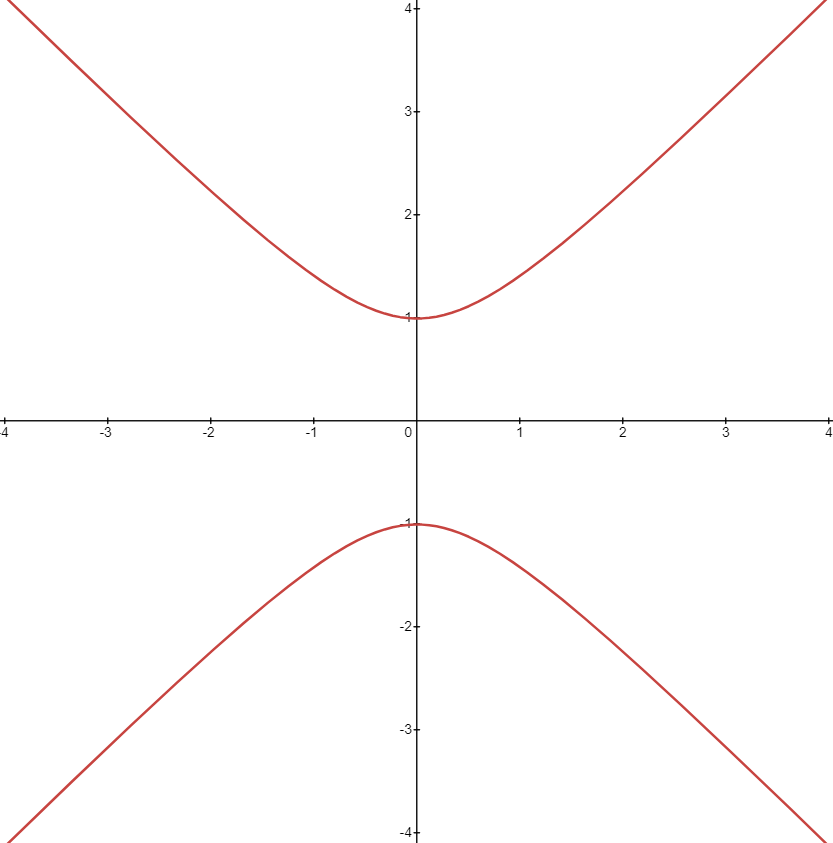
\includegraphics[width=0.5\linewidth]{picture/hyperbola=1.png}
    \caption{Hyperbola of invariant spacetime interval}
    \label{fig:hyperbolic spacetime}
\end{figure}
This means that if we connect a line from the origin to any point on this hyperbola, we should have an invariant spacetime interval. This is the hyperbola of invariant spacetime interval. We can have a series of hyperbola that represents different event and different spacetime intervals. With this graph, it would be easier to find the relationships between events. 


\section{Regions of Spacetime Diagram}
placeholder

\subsection{Speed of Causal Relationship}
There is a speed limit as to how fast causality is, and that is the speed of light. On the spacetime diagram, the region where one can have causal relation with is the region bounded by the 2 diagonal line that represents the speed of light. 

\subsection{Timelike, Spacelike, and Lightlike Events}
In Euclidean Geometry, distance is the sum of 2 squares, therefore it can never be negative.
\begin{align}
x^2 + y^2 = r^2
\end{align}
But for spacetime interval, the result could be either positive, negative, or zero depending on which parameter predominates the interaction.
\begin{align}
\Delta s^2 = -\Delta t^2 + \Delta r^2
\end{align}
Let's think of some examples to understand the difference. Let there be a train that is traveling with respect to observer in a lab frame. A spark plug flashes twice with a time separation of $\Delta t'$. For observers on the train, 2 flashes or 2 events happened on the same location, hence the spatial separation is zero. Therefore:
\begin{align}
-\Delta t'^2 = \Delta s^2 =  -\Delta t^2 + \Delta r^2
\end{align}
We see that we yield a negative number for the spacetime interval. We call this \textbf{Timelike Interval}, and the worldline connecting these 2 events are called \textbf{Timelike Worldline}. And when we have a timelike interval, we would call it the \textbf{Proper Time}\\
\newline
Similarly, we can define another similar situation. The train now has 2 spark plugs with spatial separation $\Delta r'$. For the train, 2 spark plugs would flash simultaneously, meaning that the time separation is zero for the train observer. We have the following relationship:
\begin{align}
\Delta r'^2 = \Delta s^2 = -\Delta t^2 + \Delta r^2
\end{align}
We see that the spatial separation predominates the relationship and yielding a positive spacetime interval. We call this a \textbf{Spacelike Interval}. And just like the timelike interval, we would call this spacelike interval the \textbf{Proper Distance}.\\
\newline
One thing to notice is that no worldline can connect 2 events connected by a spacelike interval. This means that 2 events connected by a spacelike interval has no causal relationship, and the sequence of which event happens first can be frame dependent as it would not violate causality.\\
\newline
Lastly, we have a special case. If the 2 events lie on the line that represents the speed of light, or when $\Delta t = \Delta r$, we will have a spacetime interval that is zero.
\begin{align}
\Delta s = 0
\end{align}
We call this a \textbf{Lightlike Interval}, since the events are located on the line that is the speed of light. Only particles that can travel at the speed of light, or influence that and propagate at the speed of light can connect 2 events tied by a lightlike interval, such as photon, and gravity. \\
\newline 
We can look at this sample diagram and intuitively understand what are the kinds of intervals. \\

\begin{itemize}
    \item Event 1 $\iff$ Event 3: Timelike Interval/Worldline, Proper time
    \item Event 1 $\iff$ Event 4: Lightlike Interval, Null Interval
    \item Event 1 $\iff$ Event 2: Spacelike Interval, proper distance 
\end{itemize}

\begin{figure}[!h]
    \centering
    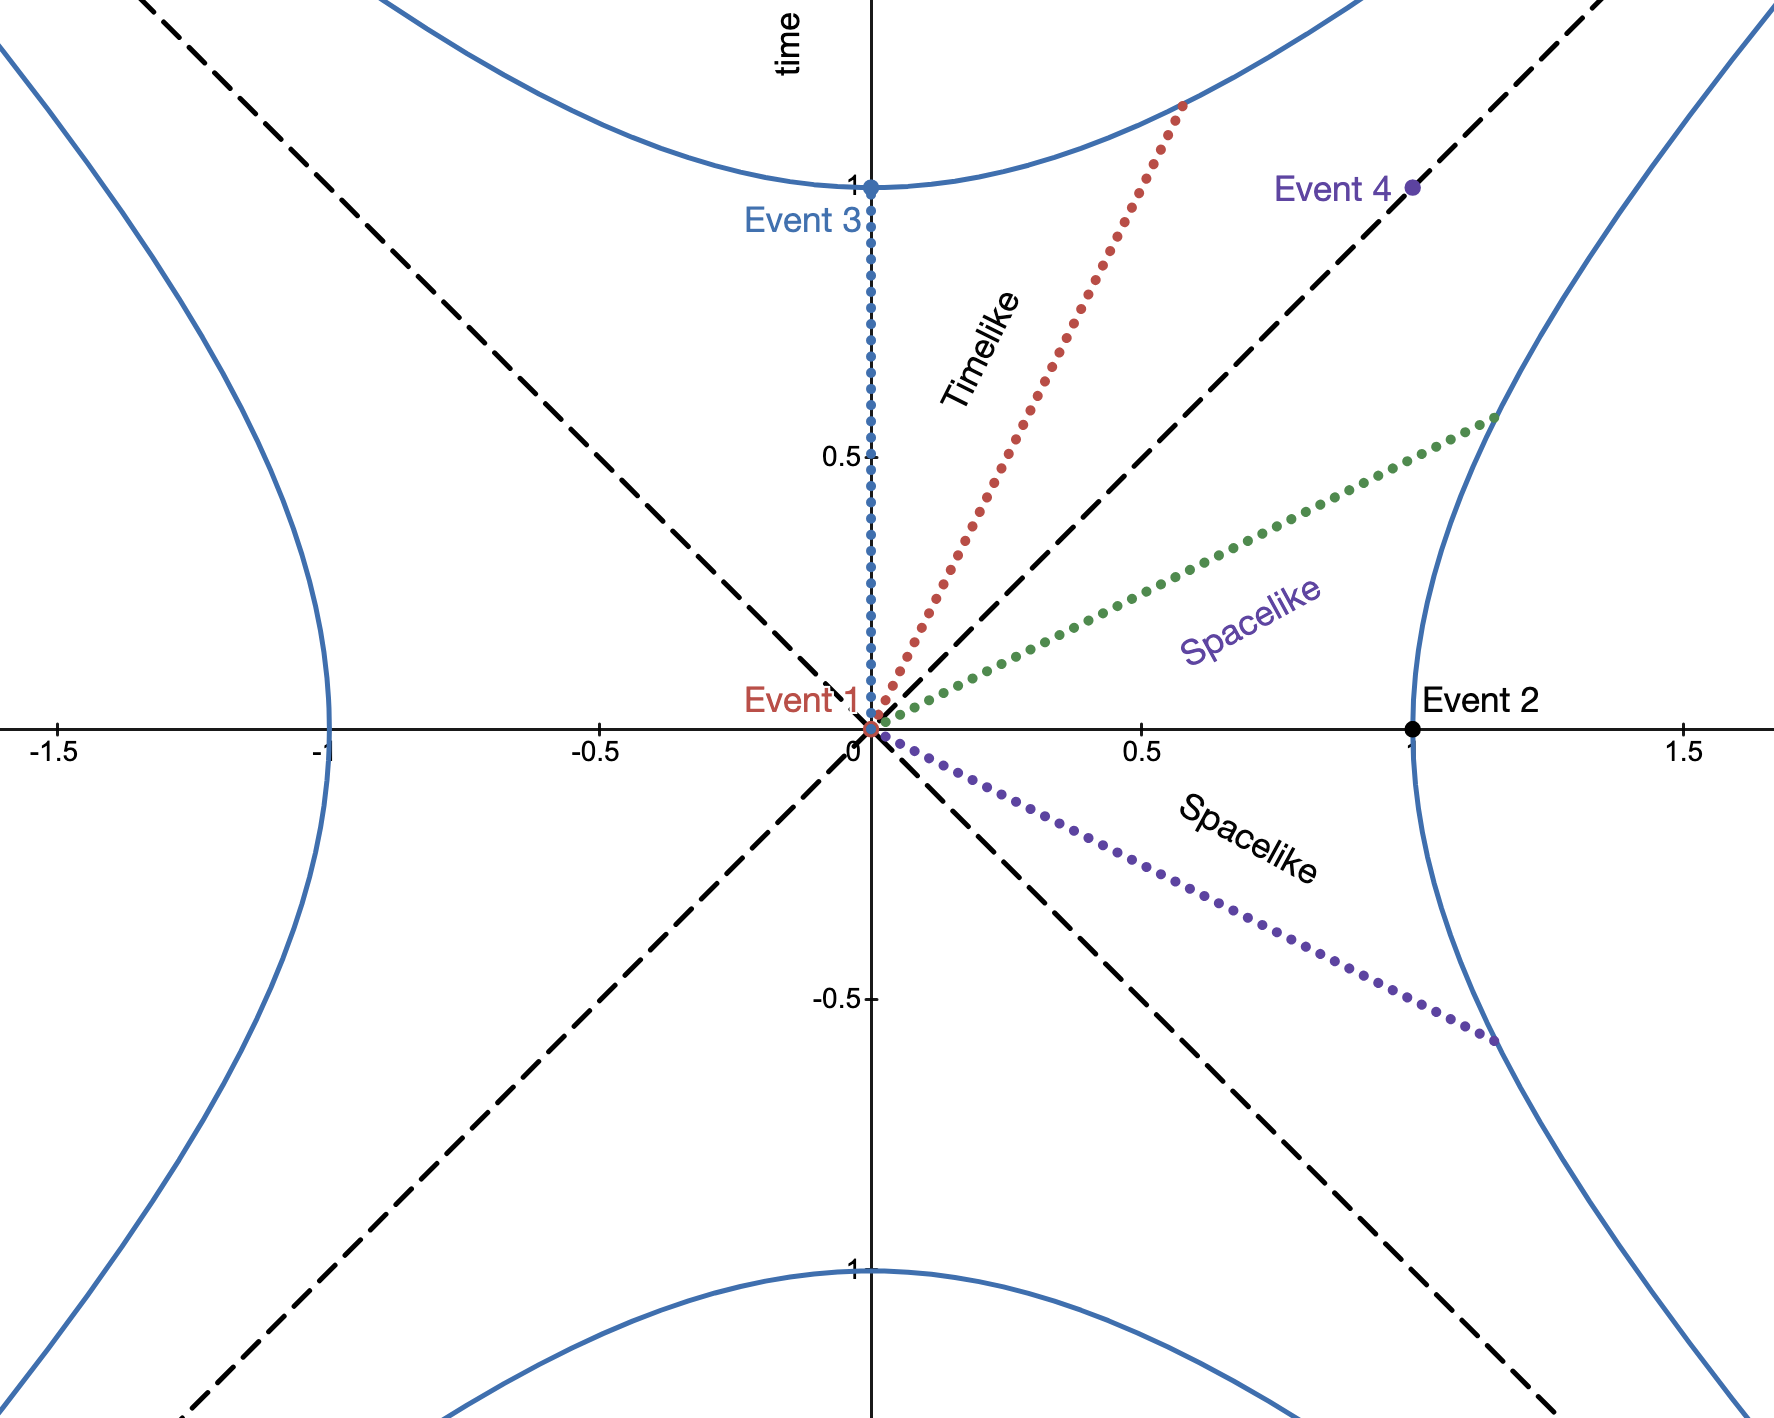
\includegraphics[width=0.5\linewidth]{picture/Spacetime diagram .png}
    \caption{Sample Diagram of different spacetime intervals}
    \label{fig:spacetime diagram}
\end{figure}

\newpage 

\subsection{Light Cone}
Since causality influence our universe at the speed of light, we can think of the speed of light and the distance it travels as the boundary of our interaction, outside which we will never be able to apply any effect. With this in mind, we can dissect our spacetime diagram into 5 different component. \\
\newline
Let us imagine we are at the origin of this spacetime diagram.
\begin{enumerate}
    \item The area shaded blue will be our \textbf{future light cone}, it contains everything that one at the origin will ever be able to alter
    \item The area shaded green is the \textbf{past light cone}, it is all the event that can have a causal relation to us.
    \item The violet boundary of the future light cone is the \textbf{future lightlike region}, where influence would have to propagate at the speed to light to alter anything on this line. Think about \textit{lightlike interval} or \textit{null interval}
    \item The red boundary of the past light cone is similar in nature to the lightlike region of the future light cone, but belongs to the past.
    \item Everything else that is not shaded is the \textbf{spacelike region}, inside which we would never be able to alter, not can it have a causal relation to us. 
\end{enumerate}

\begin{figure}[!h]
    \centering
    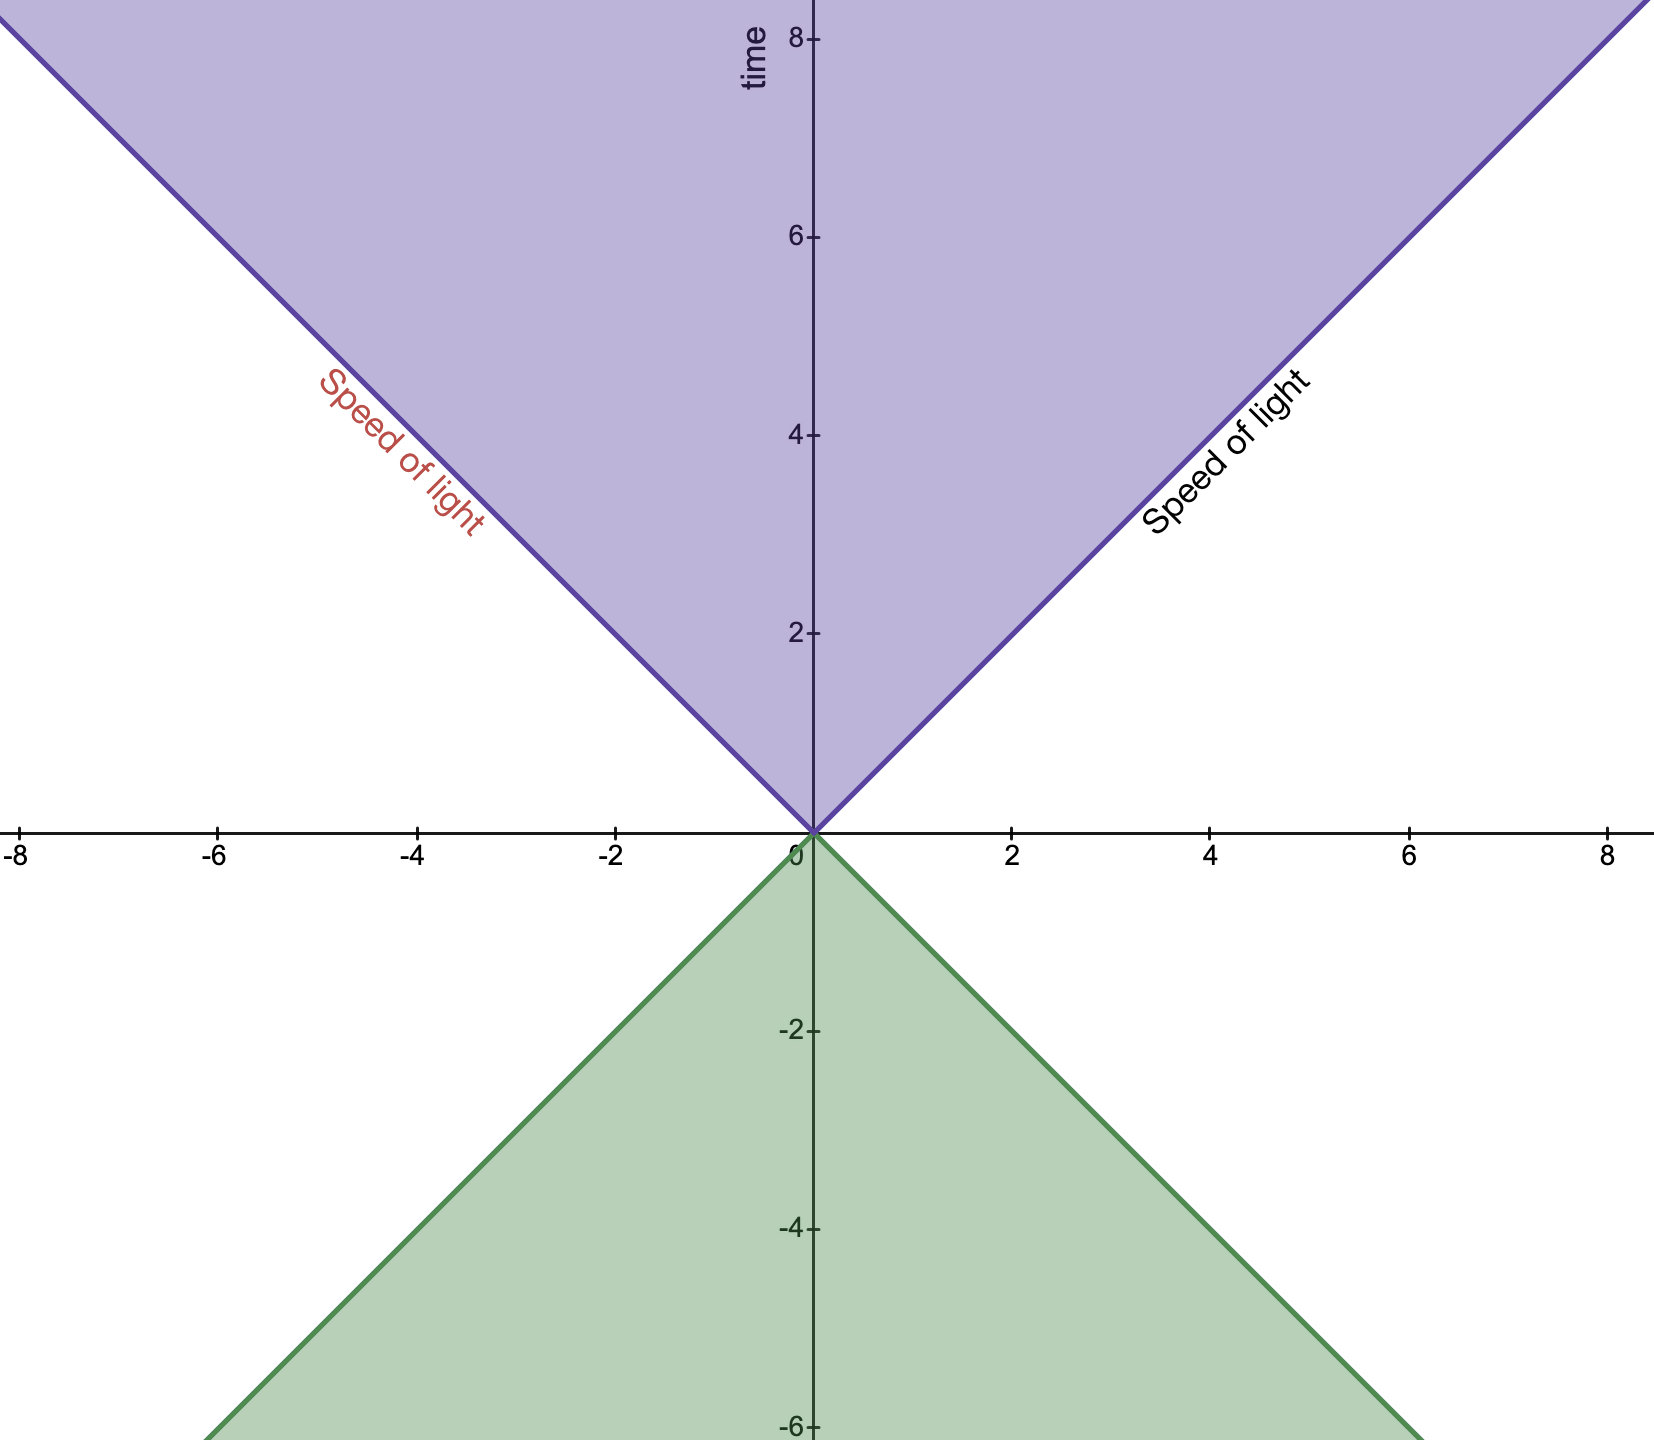
\includegraphics[width=0.5\linewidth]{picture/Light Cone.png}
    \caption{Light Cone}
    \label{fig:lightcone}
\end{figure}

\newpage

\section{Momentum-Energy Conservation}
In this chapter we would seek to treat Momentum and Energy as one group. Conservation of Momentum and Conservation of Energy, or the Newtonian way to understanding motion, fails to work when stuff is happening in relativistic speed. We therefore seek a new way to explore the conservation. We define a term \textbf{Momenergy}, or \textbf{Momentum-energy} to denote this new property.
\subsection{Relationship of Momentum and Energy}
Notice that our notation of speed $\beta$ does not involve a unit. If we consider the classical definition of momentum and energy, $\textbf{p}=m\textbf{v}$ and $E = \frac{1}{2}mv^2$, we would have momentum and energy in the same unit. \\
\newline
We should realize that momenergy is a directed quantity, or a vector, with \textbf{4 components}. It has \textbf{3 dimensions of space} that corresponds with momentum and \textbf{1 dimension of time} for energy. The direction at which the momenergy point is the directed along the worldline between 2 events.\\
\newline
Remember that there is no preferred direction for momenergy. It points at where our test particle is moving, or along the worldline. Let us denote the movement of the particle along the 4-dimensional spacetime with \textbf{spacetime displacement}. This displacement is a vector with 4 components, 1 in time and 3 in space. \\
\newline
Since the momenergy points along the worldline, its direction should be consistent for all inertial frame. And the time we would use for our spacetime displacement would the proper time along the worldline, as that is agreed upon by all inertial frame.\\
\newline
If we were to examine the spacetime diagram, we can figure out the relationship that is somewhat Pythagorean.\\

\begin{figure}[!h]
    \centering
    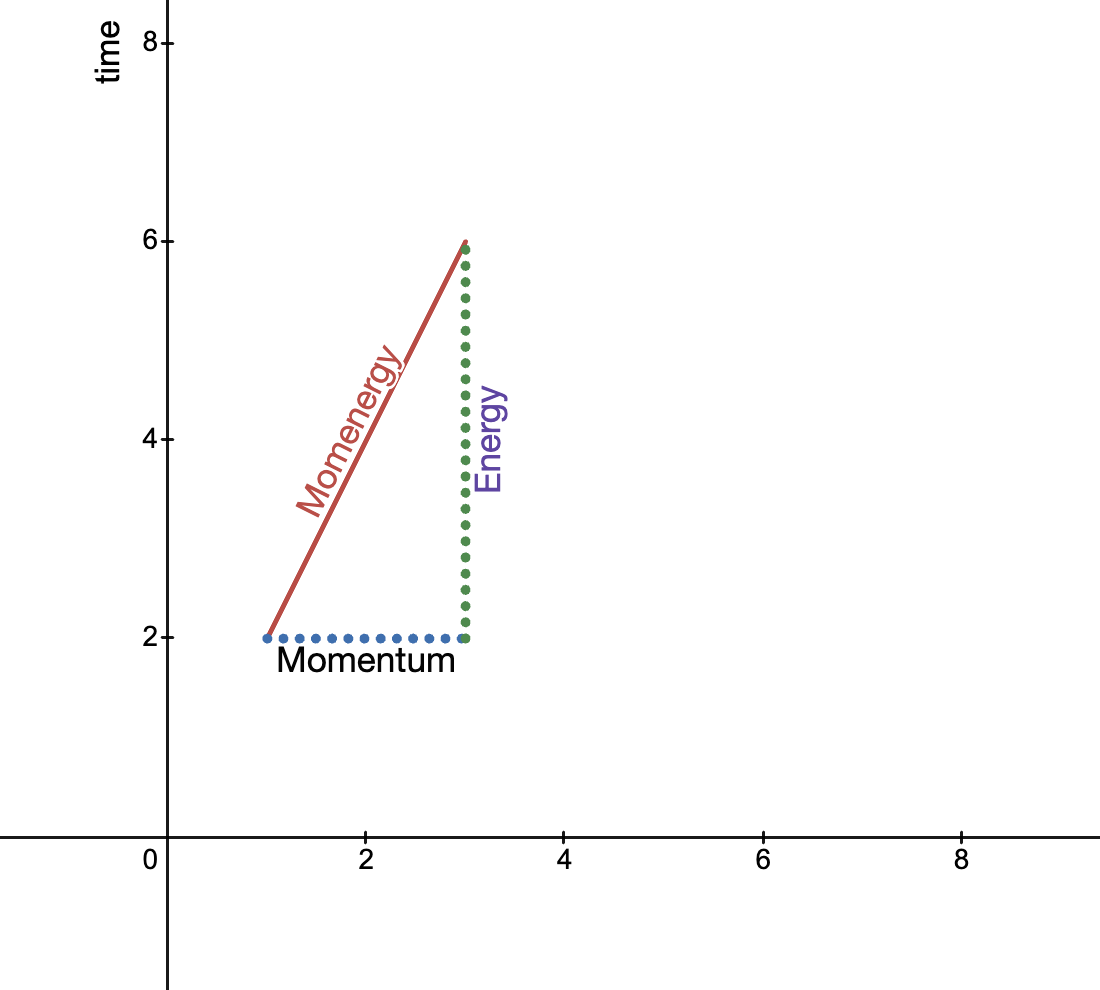
\includegraphics[width=0.5\linewidth]{picture/momentum-energy.png}
    \caption{Relationship Between Momentum and Energy}
    \label{fig:enter-label}
\end{figure}
\newpage
We can derive the following relationship. 
\begin{align}
\textbf{Momenergy} = \paren{mass}\times \frac{\paren{\text{spacetime displacement}}}{\paren{\text{proper time of displacement}}}
\end{align}
Our claim is that this momenergy would be conserved between, say, a collision. And before going to the final result, we have revisit what we have concluded so far.
\begin{enumerate}
    \item \textbf{\textit{m} units of mass pursuing a given motion carry \textit{m} times the momenergy of 1 unit of mass.} Momentum is proportional to mass.
    \item \textbf{Momenergy points in the same direction as worldline}.
    \item \textbf{Two event define a worldline between them}, think of it like how 2 points define a line segment.
    \item \textbf{Momenergy is independent of reference frame}, since spacetime interval is independent and agreed upon by all reference frame.
    \item \textbf{We define the direction and magnitude of momenergy 4-vector by 4 unit vectors,} 1 in time, 3 in space. 
    \item \textbf{The momenergy vector is defined as}
    \begin{align}
\textbf{Momenergy} = \paren{mass}\times \frac{\paren{\textbf{spacetime displacement}}}{\paren{\text{proper time of displacement}}}
\end{align}
\end{enumerate}

\subsection{Space component of momenergy, Momentum}
We have to be careful here since the numerator of this expression is actually a vector with 4 components $\tribkt{t,x,y,z}$, and is divided by a scalar \textit{proper time}.\\
\newline
We can therefore investigate momenergy of different dimension separately. Let us define proper time to be $\tau$, and $E$ be energy
s
Remember that the momenergy lies on the spacetime interval, our claim is that it has the same magnitude as the spacetime displacement. And since the magnitude of the spacetime displacement should equal to the proper time, we can see that the magnitude of momenergy is simply $\textit{m}$.
\\
\newline
We would also notice that energy and momentum is not conserved across different reference frame, but mass, or momenergy, is. Similar to what we have discussed in the invariant of spacetime interval, an object can have infinite possible momentum and energy as measured in different frames, but its spacetime interval, or mass is agreed upon by all observers. \\
\newline
Why have we not yet noticed the inconsistency of Newtonian mechanics? To answer this question, we can examine the Newtonian expression of momentum. 
\begin{align}
\textbf{p}_{Newton} = m\dydx{\textbf{r}}{t}
\end{align}
We notice that the only difference here is the use of $dt$ instead of the proper time $d\tau$. this difference is negligible and hard to detect unless the object is moving in relativistic speed. We know that 
\begin{align}
dt = \gamma d\tau
\end{align}
Therefore 
\begin{align}
E = m \dydx{t}{\tau} = \gamma m
\end{align}
\begin{align}
\textbf{p}_r = m\dydx{\textbf{r}}{\tau} = \gamma m\textbf{v}_r
\end{align}
We see that the difference does not occur until the particle moves with about $\beta=0.3$. For a high energy cosmic ray that shoots through Milky Way, it crosses the entire Milky Way in $30s$ in his own frame while $3\times 10^{12}$ has passed for Earth. The difference gets quite absurd at this speed. 

\subsection{Time component of Momenergy, Energy}
Let's investigate the time component of our 4-vector momenergy, how different is it from our classical definition?\\
\newline 
We have established previously that 
\begin{align}
E =m \dydx{t}{\tau} =\gamma m
\end{align}
As before, we consider the classical, or Newtonian definition of kinetic energy:
\begin{align}
E_{N} = \frac{1}{2}mv^2
\end{align}
How does this compare to our relativistic definition?
\begin{align}
E_{rest} = m
\end{align}
We call $E_{rest}$ the rest energy of the particle. The difference here primarily comes from the fact that, $E_{rest}$ describes the total energy a particle carries, which is a relationship not described in Newtonian mechanics that only describes the \textit{Kinetic Energy} of the Particle. We should make our definition of energy more rigorous. \\
\newline
Let $E$ be our total energy, it should have the following relationship:
\begin{align}
E = m + K
\end{align}
Where $m$ is the rest energy and $K$ is the kinetic energy. And from this relationship we can get a relativistic expression for kinetic energy K:
\begin{align}
K = E_{tot} - E_{rest} = E - m = m(\gamma - 1)
\end{align}
Now let us look back at \textit{Figure 4}, we notice that the slope of the line of momenergy is simply:
\begin{align}
v = \frac{p}{E}
\end{align}
The speed of the particle is the slope of the worldline, therefore the slope of the momenergy. \\
\newline
Now we can get the units sorted out so we can start working on the conversions. Here we will use $E_c$, $K_c$ to denote the converted energy, which should have the same unit across.

\begin{align}
E_c = Ec^2 = \gamma mc^2
\end{align}
This is the relativistic total energy of a particle 
\begin{align}
E_c = mc^2
\end{align}
This is the rest energy of a particle
\begin{align}
K_c = \frac{1}{2}m\beta^2= \frac{1}{2}mv^2c^2 
\end{align}
Here, we get to see the most famous equation of physics in its full glory. $E = mc^2$ demonstrates an incredibly large energy for any mass. But remember that Energy is not the same as mass. We must always remember that it is the rest energy $E_{rest} = mc^2$. Mass is the magnitude of the 4-vector momenergy. 
\subsection{Conservation of Momentum-Energy}
After sorting out our relativistic mechanics, we have come to a very important property that can help us study stuff happening at high speed. \textbf{The conservation of total energy.}\\
\newline
We must realize the potency of this relativistic expression of energy. It includes all sort of energies that is being converted, or transformed in the system during the event. All the interaction of energy is zipped into this \textit{proper time interval}. In the other hand, Newtonian energy is only conserved in perfectly elastic collision, as energy would be converted into heat, sound, and other sort that makes the equivalence invalid. Relativistic mechanics governs \textit{all} interaction of energy. \\
\newline
So how does this conservation translate into calculation and experimental measures?\\
\newline 
Imagine 2 particle collides, and we plot their interaction on the spacetime diagram. The only thing we need to bear in mind is that the sum of the spacetime displacement, or momenergy should add up to a constant that maintain its value before and after the collision. \\
\newpage


Not only that, since we are interested in \textit{the time part of momenergy}, or \textit{energy}, it is also conserved before and after the collision, as we can see from \textit{figure 1.5}. We call this the \textbf{conservation of the time part of momenergy}.
\begin{figure}[t]
    \centering
    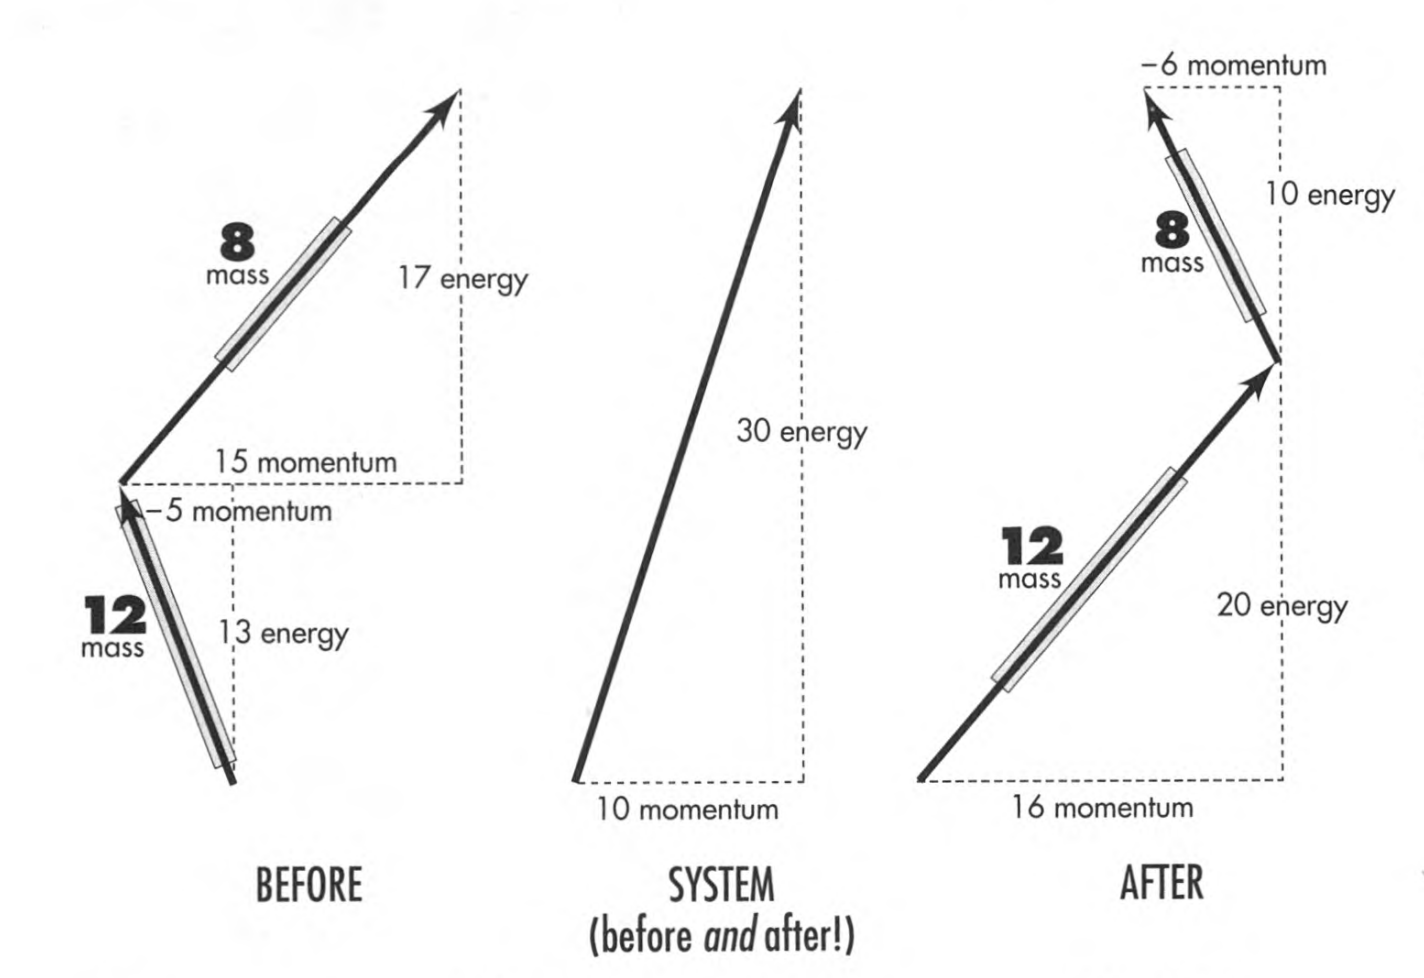
\includegraphics[width=0.5\linewidth]{picture/Momenergy of a system of particles.png}
    \caption{Momenergy of a system of particles (pg 207)}
    \label{fig:pg207}
\end{figure}\\
\newline
What about the space part of the momenergy, the momentum? As we can see from the figure above, it also stays the same before and after the collision, as measured by any inertial frame. Therefore we call this \textbf{Conservation of space part of momenergy}.
\newline
Here, we have a good opportunity to clarity the differences between \textit{invariant}, \textit{conserved}, and \textit{constant}. 
\begin{itemize}
    \item \textbf{Invariant}: A quantity is said to be invariant if it has the same value when measured by observers from reference frames in relative motion with each other. Such as the speed of light, or space time interval.
    \item \textbf{Conserved} We call a quantity conserved if before and and after an encounter, or interaction, it stays the same in a set inertial reference frame. Such as momentum and energy. It is not intrinsic to the event itself and is dependent of frame. 
    \item \textbf{Constant} We say something is constant if it is not dependent of time. Saying something is invariant is different from saying something is constant. Saying a quantity is constant means that when the quantity is recorded, it should not change after time goes on. Such as the speed limit of a highway. Observers on the International Space Station would measure a completely different speed limit for highway but that value would stay constant in his frame. 
\end{itemize}
\subsection{Summary}
Some key takeaway for this section are as follows. Let us denote momenergy with $\textbf{E}_{pE}$, and it is a vector with 4 components, 3 from space and 1 from time. 
\begin{align}
\textbf{E}_{pE} \in \R ^4 \Rightarrow \tribkt{E,p_x,p_y,p_z}
\end{align}
\begin{align}
\textbf{p} = m\dydx{\textbf{r}}{\tau} \;\;\; \textbf{r} = \tribkt{x,y,z}
\end{align}
The magnitude of the momenergy of a particle is the mass of the particle. 
\begin{align}
\abso{\textbf{E}_{pE}}^2 = m
\end{align}
And in a set frame, the components of a particle's momenergy is expressed as:
\begin{align}
E = m\dydx{t}{\tau} = \gamma m
\end{align}
And when the particle is at rest
\begin{align}
E_{rest} = m
\end{align}
\begin{align}
p_x = m\dydx{x}{\tau}\;\;\; p_y = m\dydx{y}{\tau}\;\;\; p_z = m\dydx{z}{\tau}
\end{align}
And the magnitude of the momentum can be expressed as
\begin{align}
p = \gamma \beta m
\end{align}
The total energy of the system has the following relationship, $K$ here denotes kinetic energy.
\begin{align}
E_{tot}=E_{rest} + K
\end{align}
and we can isolate $K$
\begin{align}
K = m(\gamma -1)
\end{align}
An important relationship to notice
\begin{align}
\beta = \frac{p}{E}
\end{align}
 Momentum $p$ and Energy $E$ should have the same unit.
\newpage
And the laws of conservation needs to be addressed
\begin{enumerate}
    \item \textbf{Total energy, or time part of momenergy, is conserved before and after an interaction in a given frame.}
    \item \textbf{Momentum, or space part of momenergy, is conserved before and after an interaction in a given frame. }
\end{enumerate}
\begin{figure}[!h]
    \centering
    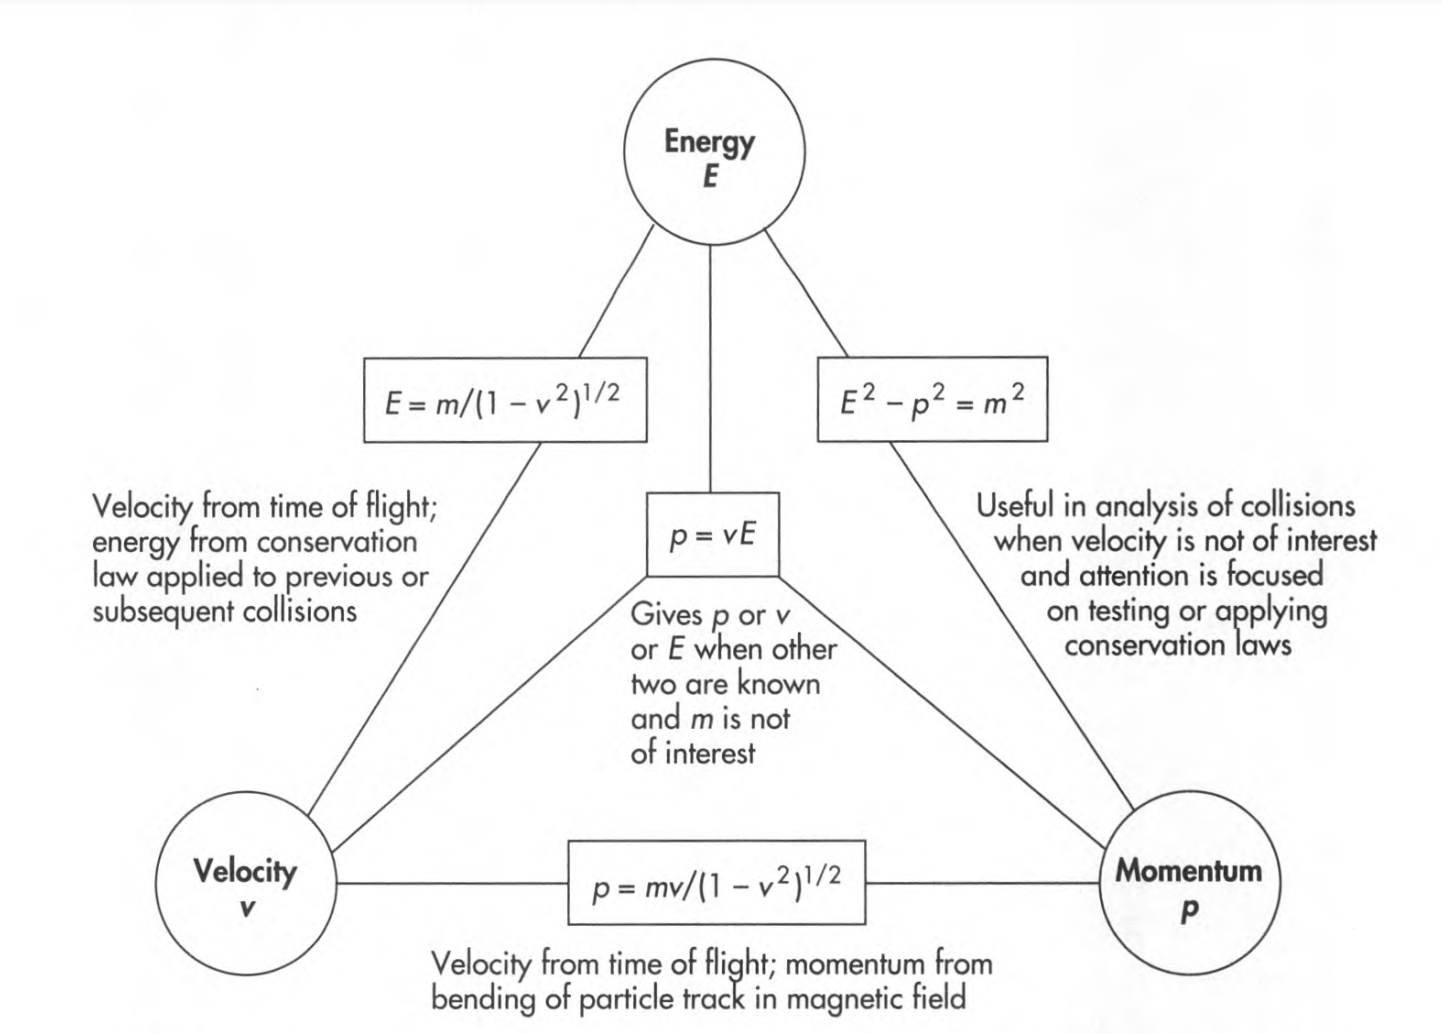
\includegraphics[width=0.5\linewidth]{picture/Momenergy relationship.png}
    \caption{Enter Caption}
    \label{fig:pEconv}
\end{figure}

\subsection{Problems}
\subsubsection{momenergy 4-vector}
For each of the following cases, write down the four components of the momentum-energy 4-vector in the given frame in the form $\tribkt{E,p_x,p_y,p_z}$. Assume that each particle has mass \textit{m}. 
\begin{enumerate}
    \item A particle moves in the positive x-direction in the lab frame with total energy equal to $5E_{rest}$
    \item Same particle as observed in a frame in which it is at rest.
    \item Another particle moves in the z-direction with momentum equal to three times its mass.
    \item Yet another particle moves in the negative y-direction with kinetic energy equal to $4m$.
    \item Still another particle moves with total energy equal to $10m$ and \{$p_x:p_y:p_z = 1:2:3$\}
\end{enumerate}
\textbf{Solutions}
\begin{enumerate}
    \item \(E_{tot}=5m\)
    \begin{align}
    K = 25m^2 - m^2 = 24m^2
    \end{align}
    \begin{align}
    \textbf{E}_{pE} = \tribkt{5m,2\sqrt{6}\;m,0,0}
    \end{align}
    \item \( E_{tot} = E_{rest} = m\)
    \item \(E_{tot}^2 = E_{rest}^2 + p^2\)
    \begin{align}
    E_{tot}^2 = 10m^2
    \end{align}
    \begin{align}
    \textbf{E}_{pE} = \tribkt{\sqrt{10}\; m, 0,0,3m}
    \end{align}
    \item \( \textbf{E}_{pE} = \tribkt{3\sqrt{3}\; m},0,-4m,0\)
    \item \(E_{tot} = 10m\)
    \begin{align}
    E_{tot}^2 = 100m^2 = \sqbkt{p_x^2+4p_x^2+9p_x^2}+m^2
    \end{align}
    \begin{align}
    p_x = \sqrt{\frac{99}{14}}m
    \end{align}
    \begin{align}
    \textbf{E}_{pE} = \tribkt{10m,\sqrt{\frac{99}{14}}\;m,2\sqrt{\frac{99}{14}}\;m,3\sqrt{\frac{99}{14}}\;m}
    \end{align}

\end{enumerate}


\section{Relativistic Interactions}
In this section we would explore interactions happened in relativistic context, such as collision, annihilation, or even creation of particle. 

\subsection{System}
We have to define a system on which we would start to do our magic of special relativity.

\subsection{Mass of the System} 
This is a very important concept to grasp in the study of relativity. We are examining \textit{rest mass} of the entire system we are interested in. It is a \textit{property} of the system, and it is an inherent characteristic that cannot be attributed to any specific entity in the system nor does it manifest in a specific form. Asking where the mass of the system is located is a poorly worded problem. Nature demands a conservation of total energy before and after an interaction, therefore we found this quality that satisfy this demand.\\
\newline
We have to realize that, although kinetic energy and momentum has been following a linear relationship, meaning we can add or subtract easily, mass addition does not follow a linear relationship in the system. Now let's do a few examples to make the concept solid. Remember, to study this system, we have to ensure it is an \textbf{isolated system}. As long as the system is isolated, we can choose an arbitraty frame to study it and will get an invariant rest mass for the system.  \\
\subsubsection{Sample Problem I}
Compute $m_{sys}$ for all the following case, assuming all the particle in question are of mass $m$ unless otherwise stated.
\begin{enumerate}
    \item System A: \\
    Particle 1: \(K = 3m \hat{\textbf{x}}\)\\
    Particle 2: \(K = 0\)
    \item System B:\\
    Particle 1: \(K = 5m \hat{\textbf{x}}\)\\
    Particle 2: \(K = 5m \hat{\textbf{x}}\)
    \item System C:\\
    Particle 1: \(E_{rest} = 3m\), \(\textbf{E} = 7m \hat{\textbf{x}}\)\\
    Particle 2: \(K = 0m \hat{\textbf{x}}\)
    \item System D:\\
    Particle 1: \(\textbf{E}=-6m\hat{\textbf{y}}\)\\
    Particle 2: \(\textbf{E}=6m\hat{\textbf{x}}\)
\end{enumerate}
\subsubsection{Solution I}
\begin{enumerate}
    \item System A:
    \begin{align}
    E_1 = 3m + m = 4m\end{align}
    \begin{align}
    p_1 = \sqrt{15}m = p_{sys}
    \end{align}
    \begin{align}
    E_{sys} = 3m + 2m = 5m
    \end{align}
    \begin{align}
    m_{sys} = \sqrt{E_{sys}^2-p_{sys}^2}=\sqrt{10}m
    \end{align}
    \item System B:\\
    Particles 1 and 2 are not in relative motion. Therefore the mass of the system is simply $m_{sys} = 2m$. Mathematical proof:
    \begin{align}
    E_1 = E_2 = 6m
    \end{align}
    \begin{align}
    E_{tot}=12m
    \end{align}
    \begin{align}
    p_1 = p_2 = \sqrt{35}m
    \end{align}
    \begin{align}
    p_{tot}=2\sqrt{35}m
    \end{align}
    \begin{align}
    m_{sys} = \sqrt{144 - 140} = 2m
    \end{align}
    \item 
\end{enumerate}

\subsection{Energy and Mass}
Energy can be transferred with mass-less medium such as photon. A photon carries only momentum but not kinetic energy. And it has a wave length of 
\begin{align}
\lambda = \frac{h}{p}
\end{align}
$h$ here is the plank constant. Also, since a photon is mass-less, it means that its momenergy points in the lightlike direction, and its motion traces the lightlike worldline. And since it has no kinetic energy, its energy can be easily expressed as 
\begin{align}
E = p 
\end{align}
Here, p represents the momentum of the photon, and E is the energy that proton carries. \\
\newline

We get to see the effect of a photon interaction when a photon scatters off an election. Compton first discovered this effect and derived a theory that quantize the energy of light, which was a monumental event in the study of quantum physics.\\
\newline
With enough energy, mass can even be conjured out of nowhere. A photon carrying $p=4m_e$ can hit an electron at rest and create a pair of $e^-$ and $e^+$, an electron and a positron. These particles would form a structure called $polyelectron$ which will keep moving in the direction of the original photon. And the photon that caused the incident would scatter and turn around going to opposite direction. This is called a \textbf{backward scattering}. \\
\newline
If you would accelerate something heavier like a proton and clash it with another proton, you can make heavier particles out of nowhere. And when a pair of matter and antimatter, such as electron and position, touches each other, they would annihilate and convert all its mass to energy. This is probably the most efficient way of obtaining energy. Way more efficient than nuclear fission and fusion which also harvest the conversion of mass to energy. \\
\newline
Do keep in mind that energy and mass are not always convertible, and they have to comply with the 2 fundamental laws in relativity:
\begin{itemize}
    \item \textbf{Invariant of Momenergy of isolated system, and conservation of Momenergy before and after interactions in an isolated system.}
    \item \textbf{The invariant magnitude of the momenergy of a particle equals the rest mass of that particle. }
\end{itemize}

\subsection{Wrapping up: Questions to think about}
This section will wrap up our study so far nicely. It will be consisted of questions and answers to some interesting topics. 
\begin{enumerate}

    \item Does an isolated system have the same mass as observed in every inertial (free-float) reference frame?
    \item[Answer:] Yes, think of rest mass as the spacetime interval, where the space interval is momentum and time interval is energy. The mass should be invariant across reference frame just like spacetime interval.
    \item Does its energy have the same value in every inertial frame?
    \item[Answer:]No, momentum and energy can vary in different reference frame. 
    \item Does energy equal zero for an object of zero mass, such as a photon?
    \item[Answer:]No, Photons obviously have energy as discussed previously. Its energy equals its momentum. 
    \item Can a photon — that has no mass— give mass to an absorber?
    \item[Answer:] This is certainly possible, such as the example of the positron electron pair created by the photon. Mass was created. 
    \item Invariance of mass; Is that feature of nature the same as the principle that all electrons in the universe have the same mass?
    \item[Answer:] The invariance of mass is describing a more general case than the elementary particles. It says that for any reference frame, even if the observation for kinetic energy and momentum is different, everyone should come to the same conclusion as to what the rest mass it.
    \item Momenergy: Is that a richer concept than mass?
    \item[Answer:] Yes it is. It describes the direction of the particle in the spacetime diagram rather than being a scalar that provides no additional information. 
\end{enumerate}

\subsection{Problems}
WIP

\chapter{Intro to Electrodynamics - Griffiths}

\section{Electrodynamics and Relativity (12.1)}

\subsection{12.1 The Special Theory of Relativity}

    \subsubsection{12.1.1 Einstein’s Postulates}
            \begin{enumerate}
                \item \textbf{The principle of relativity.} The laws of physics apply in all inertial reference systems.
                \item \textbf{The universal speed of light.} The speed of light in vacuum is the same for all inertial observers, regardless of the motion of the source.
            \end{enumerate}
     Although it developed historically out of Einstein’s contemplation of electrodynamics, the special theory is not limited to any particular class of phenomena—rather, it is a description of the space-time “arena” in which all physical phenomena take place. And in spite of the reference to the speed of light
    in the second postulate, relativity has nothing to do with light: c is a fundamental velocity, and it happens that light travels at that speed, but it is perfectly possible to conceive of a universe in which there are no electric charges, and hence no electromagnetic fields or waves, and yet relativity would still prevail.
    
\subsubsection{12.1.2 The Geometry of Relativity}
    \begin{enumerate}
        \item \textbf{The relativity of simultaneity}: Two events that are simultaneous in one inertial system are not, in general, simultaneous in another. An \textbf{observation} is an artificial reconstruction after the fact, when all the data are in, and it doesn’t depend on where the observer is located. In fact, a wise observer will avoid the whole problem by stationing assistants at strategic locations, each equipped with a watch synchronized to a master clock, so that time measurements can be made right at the scene.
        \item \textbf{Time dilation}: Moving clocks run slow. $\bar{\Delta t} = \sqrt{1 - \frac{v^2}{c^2}}\Delta t$. Evidently, the time elapsed between the same two events (light leaves bulb, and light strikes center of floor) is different for two observers (inside the train and outside). In fact, the interval recorded on the train clock, $\bar{t}$, is shorter by the factor $\gamma \equiv \frac{1}{\sqrt{1 - \frac{v^2}{c^2}}}$. 
        Because moving clocks are not synchronized, it is essential when checking time dilation to focus attention on a single moving clock. All moving clocks runs low by the same factor, but you can’t start timing on one clock and then switch to another because they weren’t in step to begin with. But you can use as many stationary clocks (stationary with respect to you, the observer) as you please, for
        they are properly synchronized (moving observers would dispute this, but that’s their problem).
        \item \textbf{Lorentz contraction}: Moving objects are shortened. Dimensions perpendicular to the velocity are not contracted. $\bar{x} = x \sqrt{1 - \frac{v^2}{c^2}}$. And the relativistic velocity addition formula of A wrt C (ground), and A wrt B (train) is:
        \begin{align}
        v_{AC} = \frac{v_{AB} + v_{BC}}{1 + \frac{v_{AB} v_{BC}}{c^2}}
        \end{align}
    \end{enumerate}
    
\subsubsection{12.1.3 The Lorentz Transformations}
    Suppose we know the coordinates $(x, y, z, t)$ of a particular event $E$ in one inertial system $S$, and we would like to calculate the coordinates $(\bar{x}, \bar{y}, \bar{z}, \bar{t})$ of that same event in some other inertial system $\bar{S}$. What we need is a “dictionary” for translating from the language of $S$ to the language of $\bar{S}$. We may as well orient our axes, so that $\bar{S}$ slides along the $x$ axis at speed $v$. If we “start the clock” $(t = 0)$ at the moment the origins $(O $ and $ \bar{O})$ coincide, then at time $t$, $\bar{O}$ will be a distance $vt$ from $O$, hence the Lorentz Transformations:
    
    \begin{enumerate}
        \item $\bar{x} = \gamma (x - vt)$
        \item $\bar{y} = y$
        \item $\bar{z} = z$
        \item $\bar{t} = \gamma \left( t - \frac{v}{c^2} x \right)$
    \end{enumerate}
    
    \textbf{Rules for Translating Angles:} There is no universal rule for translating angles — you have to know whether it’s an angle made by a velocity vector $\mathbf{\tan{\theta}=\frac{u_y}{u_x}=\frac{1}{\gamma}\frac{\bar{u}_y}{\bar{u}_x+v}}$ or a position vector $\mathbf{\tan{\theta}=\gamma\frac{\sin{\bar{\theta}}}{\cos{\bar{\theta}}}}$.]
    
\subsubsection{12.1.4 The Structure of Spacetime}
    \begin{enumerate}
        \item \textbf{Four-vectors.} \\
            The Lorentz transformations take on a simpler appearance when expressed in matrix form (where $x^0=ct, \beta = \frac{v}{c}, x^1=x, x^2=y, x^3=z$): 
            \begin{align}
            \begin{pmatrix}
            \bar{x}^0 \\
            \bar{x}^1 \\
            \bar{x}^2 \\
            \bar{x}^3
            \end{pmatrix}
            =
            \begin{pmatrix}
            \gamma & -\gamma\beta & 0 & 0 \\
            -\gamma\beta & \gamma & 0 & 0 \\
            0 & 0 & 1 & 0 \\
            0 & 0 & 0 & 1
            \end{pmatrix}
            \begin{pmatrix}
            x^0 \\
            x^1 \\
            x^2 \\
            x^3
            \end{pmatrix}
            \end{align}   
            Letting Greek indices run from 0 to 3, this can be distilled into a single equation:
            \begin{align}
            \bar{x}^\mu = \sum_{\nu=0}^{3} (\Lambda^\mu_{\ \nu}) x^\nu,
            \end{align}
        
            where $\Lambda$ is the \textbf{Lorentz transformation matrix} (the superscript $\mu$ labels the row, the subscript $\nu$ labels the column). \\
            The \textbf{four-dimensional scalar product} (is invariant under $\Lambda$ just like ordinary dot product is invariant under rotation): 
            \begin{align} 
            -a^0b^0+a^1b^1+a^2b^2+a^3b^3 = -a^0b^0 + \mathbf{a \cdot b} 
            \end{align}
            Introduce \textbf{covariant} vector $a_{\mu}$ , which differs from \textbf{contravariant}  $a^{\mu}$ only in the sign of zeroth component:
            \begin{align}
            a_{\mu}=(a_0, a_1, a_2, a_3)=(-a^0, a^1, a^2, a^3)
            \end{align} Note, that raising or lowering a temporal index costs a minus sign $(a_0=-a^0)$.  Formally the \textbf{Minkowski metric}, 
            \begin{align}
            a_{\mu} = \sum_{\nu=0}^{3} g_{\mu\nu} a^\nu , \quad \text{where} \quad g_{\mu\nu} \equiv
            \begin{pmatrix}
            -1 & 0 & 0 & 0 \\
            0 & 1 & 0 & 0 \\
            0 & 0 & 1 & 0 \\
            0 & 0 & 0 & 1
            \end{pmatrix}
            \end{align}
            The scalar product can now be written with summation symbol,
            \begin{align}
            \sum_{\mu=0}^{3} a^{\mu} b_\mu \quad \text{ or, more compactly, } \quad a^\mu b_\mu =a_\mu b^\mu
            \end{align}
            This is called the \textbf{Einstein summation convention}. Note \textbf{rapidity} (rapidity add, whereas velocities dont): 
            \begin{align}
            \theta \equiv \tanh^{-1}{v/c}
            \end{align}
    
        \item \textbf{The invariant interval}\\
            If \(a^\mu a_\mu > 0\), \(a^\mu\) is called spacelike. \\
            If \(a^\mu a_\mu < 0\), \(a^\mu\) is called timelike. \\
            If \(a^\mu a_\mu = 0\), \(a^\mu\) is called lightlike. \\
            
            Suppose event A occurs at \((x^0_A, x^1_A, x^2_A, x^3_A)\), and event B at \((x^0_B, x^1_B, x^2_B, x^3_B)\).
            The difference,
            \begin{align}
            \Delta x^\mu \equiv x^\mu_A - x^\mu_B,
            \end{align}
            is the displacement 4-vector. The scalar product of \(\Delta x^\mu\) with itself is called the invariant interval between two events:
            
            \begin{align}
            I \equiv (\Delta x)^\mu (\Delta x)_\mu = -(\Delta x^0)^2 + (\Delta x^1)^2 + (\Delta x^2)^2 + (\Delta x^3)^2 = -c^2t^2 + d^2,
            \end{align}
            
            where \(t\) is the time difference between the two events and \(d\) is their spatial separation.\\
            If the displacement between two events is timelike (\(I < 0\)), there exists an inertial system (accessible by Lorentz transformation) in which they occur at the same point. For if I hop on a train going from (A) to (B) at the speed \(v = \frac{d}{t}\), leaving event A when it occurs, I shall be just in time to pass B when it occurs; in the train system, A and B take place at the same point. You cannot do this for a spacelike interval, of course, because \(v\) would have to be greater than \(c\), and no observer can exceed the speed of light (\(\gamma\) would be imaginary and the Lorentz transformations would be nonsense). On the other hand, if the displacement is spacelike (\(I > 0\)), then there exists a system in which the two events occur at the same time (see Prob. 12.21). And if the displacement is lightlike (\(I = 0\)), then the two events could be connected by a light signal.
            
        \item \textbf{Space-time diagrams}
            \\Under rotations about the \(z\) axis, a point \(P\) in the \(xy\) plane describes a circle: the locus of all points a fixed distance \(r = \sqrt{x^2 + y^2}\) from the origin. Under Lorentz transformations, however, it is the interval \(I = (x^2 - c^2t^2)\) that is preserved, and the locus of all points with a given value of \(I\) is a hyperbola. 
            When you perform a Lorentz transformation (that is, when you go into a moving inertial system), the coordinates \((x, t)\) of a given event will change to \((\bar{x}, \bar{t})\), but these new coordinates will lie on the same hyperbola as \((x, t)\). \vspace{1 cm}
            \begin{center}
                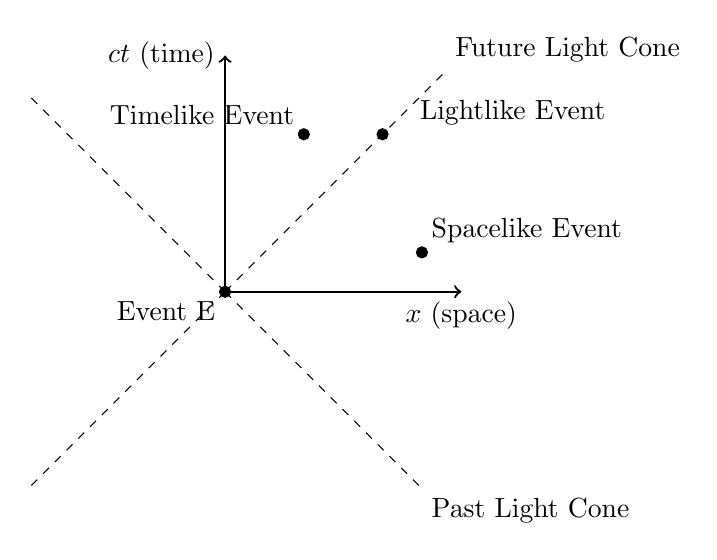
\begin{tikzpicture}[scale=1]
                    % Draw axes
                    \draw[thick,->] (0,0) -- (3,0) node[anchor=north] {$x$ (space)};
                    \draw[thick,->] (0,0) -- (0,3) node[anchor=east] {$ct$ (time)};
                
                    % Draw light cone
                    \draw[dashed] (0,0) -- (2.8,2.8) node[anchor=south west] {Future Light Cone};
                    \draw[dashed] (0,0) -- (-2.5,2.5);
                    \draw[dashed] (0,0) -- (2.5,-2.5) node[anchor=north west] {Past Light Cone};
                    \draw[dashed] (0,0) -- (-2.5,-2.5);
                
                    % Timelike separated event
                    \filldraw[black] (1,2) circle (2pt) node[anchor=south east] {Timelike Event};
                
                    % Lightlike separated event
                    \filldraw[black] (2,2) circle (2pt) node[anchor=south west] {\quad Lightlike Event};
                
                    % Spacelike separated event
                    \filldraw[black] (2.5,0.5) circle (2pt) node[anchor=south west] {Spacelike Event};
                
                    % Origin Event
                    \filldraw[black] (0,0) circle (2pt) node[anchor=north east] {Event E};
                \end{tikzpicture}
            \end{center}

             \textbf{Conclusion}: In terms of the space-time diagram, an event on the upper sheet of a timelike hyperboloid definitely occurred after (\( 0, \bm{0} \)), and one on the lower sheet certainly occurred before; but an event on a spacelike hyperboloid occurred at positive $t$, or negative $-t$, depending on your reference frame.The displacement between causally related events is always timelike, and their temporal ordering is the same for all inertial observers.
        \end{enumerate}

\subsection{12.2 Relativistic Mechanics}

    \subsubsection{12.2.1 Proper Time and Proper Velocity}      
        As you progress along your world line (\(\tau\) the time associated with the moving object -\textbf{proper time}), your watch runs slow; while the clock on the wall ticks off an interval \(dt\), your watch only advances \(d\tau\):
        
        \begin{align}
        d\tau = \sqrt{1 - \frac{u^2}{c^2}} \, dt.
        \end{align}
        
        The hybrid quantity (distance measured on the ground, over time measured in the airplane) is called \textbf{proper velocity}; for contrast, I’ll call \(u\) the ordinary velocity. The two are related by:
        
        \begin{align}
        \eta = \frac{u}{\sqrt{1 - \frac{u^2}{c^2}}}.
        \end{align}
        
        From a theoretical standpoint, however, proper velocity has an enormous advantage over ordinary velocity: it transforms simply, when you go from one inertial system to another. In fact, \(\eta\) is the spatial part of a 4-vector,
        
        \begin{align}
        \eta^\mu \equiv \frac{dx^\mu}{d\tau}=\gamma(c, v_x, v_y, v_z)
        \end{align}
        
        whose zeroth component is:
        
        \begin{align}
        \eta^0 = \frac{dx^0}{d\tau} = c \frac{dt}{d\tau} = \frac{c}{\sqrt{1 - \frac{u^2}{c^2}}}
        \end{align}
        
        for the numerator, \(dx^\mu\), is a displacement 4-vector, while the denominator, \(d\tau\), is invariant. Thus, for instance, when you go from system \(S\) to system \(\bar{S}\), moving at speed \(v\) along the common \(x\)\(\bar{x}\) axis:
        
        \begin{align}
        \begin{aligned}
        \bar{\eta}^0 &= \gamma (\eta^0 - \beta \eta^1), \\
        \bar{\eta}^1 &= \gamma (\eta^1 - \beta \eta^0), \\
        \bar{\eta}^2 &= \eta^2, \\
        \bar{\eta}^3 &= \eta^3.
        \end{aligned}
        \end{align}
        More generally,
        
        \begin{align}
        \bar{\eta}^\mu = \Lambda^\mu_{\ \nu} \eta^\nu, \quad
        \end{align}
        
        \(\eta^\mu\) is called the proper velocity 4-vector, or simply the 4-velocity.
        
        By contrast, the transformation rule for ordinary velocities is quite cumbersome:
        
        \begin{align}
        \begin{aligned}
        \bar{u}_x &= \frac{d\bar{x}}{d\bar{t}} = \frac{u_x - v}{1 - \frac{vu_x}{c^2}}, \\
        \bar{u}_y &= \frac{d\bar{y}}{d\bar{t}} = \frac{u_y}{\gamma \left(1 - \frac{vu_x}{c^2}\right)}, \\
        \bar{u}_z &= \frac{d\bar{z}}{d\bar{t}} = \frac{u_z}{\gamma \left(1 - \frac{vu_x}{c^2}\right)}.
        \end{aligned} \quad (12.45)
        \end{align}
        
        The reason for the added complexity is plain: we’re obliged to transform both the numerator \(dl\) and the denominator \(dt\), whereas for proper velocity, the denominator \(d\tau\) is invariant, so the ratio inherits the transformation rule of the numerator
        alone.
        
    \subsubsection{12.2.2 Relativistic Energy and Momentum}
        \textbf{Relativistic momentum} of an object of mass \(m\) traveling at (ordinary) velocity \(u\):
        
        \begin{align}
        \bm{p} \equiv m\eta = \frac{mu}{\sqrt{1 - \frac{u^2}{c^2}}}
        \end{align}
        
        Relativistic momentum is the spatial part of a 4-vector,
        
        \begin{align}
        p^\mu \equiv m\eta^\mu,
        \end{align}
        
        with the temporal component,
        
        \begin{align}
        p^0 = m\eta^0 = \frac{mc}{\sqrt{1 - \frac{u^2}{c^2}}}
        \end{align}
        
        Einstein identified \(p^0c\) as \textbf{relativistic energy}:
        
        \begin{align}
        E \equiv \frac{mc^2}{\sqrt{1 - \frac{u^2}{c^2}}}
        \end{align}
        
        Notice that the relativistic energy is nonzero even when the object is stationary; we call this rest energy:
        
        \begin{align}
        E_\text{rest} \equiv mc^2
        \end{align}
        
        The remainder, which is attributable to the motion, is kinetic energy:
        
        \begin{align}
        E_\text{kin} \equiv E - mc^2 = mc^2 \left(\frac{1}{\sqrt{1 - \frac{u^2}{c^2}}} - 1\right)
        \end{align}

        \begin{center}
            \textbf{In every closed system, the total relativistic energy and momentum are conserved.}
        \end{center}
        
        The scalar product of \( p^\mu \) with itself is
        
        \begin{align}
        p^\mu p_\mu = -(p^0)^2 + (\bm{p} \cdot \bm{p}) = -m^2c^2
        \end{align}
        
        In terms of the relativistic energy and momentum,
        
        \begin{align}
        E^2 - p^2c^2 = m^2c^4 
        \end{align}
        
        This result is extremely useful, for it enables you to calculate \(E\) (if you know \( p \equiv |\bm{p}| \)), or \( p \) (knowing \( E \)), without ever having to determine the velocity. If you know the energy and momentum of a particle, the velocity is: 
        \begin{align}
        \bm{v}=\frac{\bm{p}c^2}{E}
        \end{align}
        
    \subsubsection{12.2.3 Relativistic Kinematics}
    \subsubsection{12.2.4 Relativistic Dynamics}

        Newton’s first law is built into the principle of relativity. His second law, in the form
        \begin{align}
        \bm{F} = \frac{d\bm{p}}{dt} =\frac{m}{\sqrt{1 - \frac{u^2}{c^2}}} \left[ \mathbf{a} + \frac{\mathbf{u}(\mathbf{u} \cdot \mathbf{a})}{c^2 - u^2} \right]
        \end{align}
        
        retains its validity in relativistic mechanics, provided we use the relativistic momentum.
        Work, as always, is the line integral of the force:
        
        \begin{align}
        W \equiv \int \bm{F} \cdot d\bm{l}.
        \end{align}
        
        The work-energy theorem (“the net work done on a particle equals the increase in its kinetic energy”) holds relativistically:
        
        \begin{align}
        W = \int \frac{d\bm{p}}{dt} \cdot d\bm{l} = \int \frac{d\bm{p}}{dt} \cdot \frac{d\bm{l}}{dt} dt = \int \frac{d\bm{p}}{dt} \cdot \bm{u} \, dt= \int \frac{dE}{dt} dt = E_{\text{final}} - E_{\text{initial}}.
        \end{align}
        
        (Since the rest energy is constant, it doesn’t matter whether we use the total energy, here, or the kinetic energy.)
        
        Unlike the first two, Newton’s third law does not, in general, extend to the relativistic domain. Indeed, if the two objects in question are separated in space, the third law is incompatible with the relativity of simultaneity. For suppose the force of A on B at some instant \(t\) is \(\bm{F}(t)\), and the force of B on A at the same instant is \(-\bm{F}(t)\); then the third law applies in this reference frame. But a moving observer will report that these equal and opposite forces occurred at different times; in his system, therefore, the third law is violated.
        
        Because \(\bm{F}\) is the derivative of momentum with respect to ordinary time, both the numerator and the denominator must be transformed. Thus the \(x\) component:
        
        \begin{align}
        \bar{F}_x = \frac{d \bar{p}_x}{d \bar{t}} = \frac{\gamma dp_x - \gamma\beta dp^0}{\gamma dt -  \frac{\gamma\beta}{c} dx} = \frac{\frac{dp_x}{dt} - \beta \frac{ dp^0}{dt}}{1 - \frac{\beta}{c}\frac{dx}{dt}} = \frac{F_x - \frac{\beta}{c}(\frac{dE}{dt})}{1 - \frac{\beta u_x}{c}}.
        \end{align}
        and the \(y\) and \(z\) components:
        \begin{align}
        \bar{F}_y = \frac{F_y}{\gamma (1 - \beta u_x/c)}, \hspace{2cm} \bar{F}_z = \frac{F_z}{\gamma (1 - \beta u_x/c)}. 
        \end{align}      
        
        We calculated \(\frac{dE}{dt}\) using \(\frac{d\bm{p}}{dt} \cdot \bm{u} = \bm{F} \cdot \bm{u}\); putting that in:
        
        \begin{align}
        \bar{F}_x = \frac{F_x - \beta (\bm{u} \cdot \bm{F})/c}{1 - \beta u_x/c}.
        \end{align}
        
        In one special case, these equations are reasonably tractable: If the particle is (instantaneously) at rest in \(S\), so that \(\bm{u} = 0\), then:
        
        \begin{align}
        \bar{\bm{F}}_\perp = \frac{1}{\gamma} \bm{F}_\perp, \quad \bar{\bm{F}}_\parallel = \bm{F}_\parallel.
        \end{align}
        
        We introduce a “proper” force, analogous to proper velocity, which is the derivative of momentum with respect to proper time:
        
        \begin{align}
        K^\mu \equiv \frac{dp^\mu}{d\tau}. \quad (12.68)
        \end{align}
        
        This is called the Minkowski force; it is plainly a 4-vector, since \(p^\mu\) is a 4-vector and proper time is invariant. The spatial components of \(K^\mu\) are related to the “ordinary” force by:
        
        \begin{align}
        \bm{K} = \left(\frac{dt}{d\tau}\right) \frac{d\bm{p}}{dt} = \frac{1}{\sqrt{1 - \frac{u^2}{c^2}}} \bm{F}, \quad (12.69)
        \end{align}
        
        while the zeroth component,
        
        \begin{align}
        K^0 = \frac{dp^0}{d\tau} = \frac{1}{c} \frac{dE}{d\tau},
        \end{align}
        
        is, apart from the \(1/c\), the (proper) rate at which the energy of the particle increases—in other words, the (proper) power delivered to the particle.

        In classical mechanics, the total momentum (\(\bm{P}\)) of a collection of interacting particles can be expressed as the total mass (\(M\)) times the velocity of the center-of-mass:
        
        \begin{align}
        \bm{P} = M \frac{d\bm{R}_\text{m}}{dt}.
        \end{align}
        
        In relativity, the center-of-mass (\(\bm{R}_\text{m} = \frac{1}{M} \sum m_i \bm{r}_i\)) is replaced by the \textbf{center-of-energy} (\(\bm{R}_\text{e} = \frac{1}{E} \sum E_i \bm{r}_i\), where \(E\) is the total energy), and \(M\) by \(E/c^2\):
        
        \begin{align}
        \bm{P} = \frac{E}{c^2} \frac{d\bm{R}_\text{e}}{dt}.
        \end{align}
        
        \(\bm{P}\) now includes all forms of momentum, and \(E\) all forms of energy—not just mechanical, but also whatever may be stored in the fields.
        
\chapter{Intro to Elementary Particles - Griffiths}

    \section{Relativistic Kinematics (Chapter 3)}
        \subsection{3.2 Four-vectors}
            \subsubsection{1. Tensor Rank and Components}
                \begin{itemize}
                    \item \textbf{Second-Rank Tensor (e.g., \( S^{\mu \nu} \))}:
                    \begin{itemize}
                        \item A second-rank tensor has two indices (e.g., \( \mu \) and \( \nu \)).
                        \item In four-dimensional spacetime, where each index can take four values (0, 1, 2, 3), a second-rank tensor has \( 4 \times 4 = 16 \) components.
                        \item It transforms with two factors of the transformation matrix \( A \):
                        \begin{align}
                        S'^{\mu \nu} = A^\mu_{\ \alpha} A^\nu_{\ \beta} S^{\alpha \beta}.
                        \end{align}
                        \end{itemize}
                
                    \item \textbf{Third-Rank Tensor (e.g., \( T^{\mu \nu \rho} \))}:
                    \begin{itemize}
                        \item A third-rank tensor has three indices (e.g., \( \mu \), \( \nu \), and \( \rho \)).
                        \item It has \( 4^3 = 64 \) components and transforms with three factors of the transformation matrix \( A \):
                        \begin{align}
                        T'^{\mu \nu \rho} = A^\mu_{\ \alpha} A^\nu_{\ \beta} A^\rho_{\ \gamma} T^{\alpha \beta \gamma}.
                        \end{align}
                    \end{itemize}
                \end{itemize}
            
            \subsubsection{2. Hierarchy of Tensors}
            
                \begin{itemize}
                    \item \textbf{Scalars} are tensors of rank zero. They have no indices and are invariant under transformations.
                    \item \textbf{Vectors} are tensors of rank one, with a single index (e.g., \( V^\mu \)).
                    \item Higher-rank tensors follow the pattern, with more indices and correspondingly more components.
                \end{itemize}
            
            \subsubsection{}section*{3. Covariant, Mixed, and Symmetric Tensors}
            
                \begin{itemize}
                    \item \textbf{Covariant Tensor}: A tensor with all lower indices (e.g., \( S_{\mu \nu} \)). These indices are obtained by lowering the indices of a \textbf{contravariant tensor} (with upper indices) using the metric tensor \( g_{\mu \nu} \). Lowering an index can involve a change in sign for spatial indices in a metric with signature \((+, -, -, -)\).
                    \begin{align}
                        s_{\mu \nu} = g_{\mu k} g_{\nu \lambda} s^{k \lambda};
                    \end{align}
                    \item \textbf{Mixed Tensor}: A tensor that has both upper and lower indices (e.g., \( T^{\mu}_{\ \nu} \)). This tensor can result from contracting a higher-rank tensor.
                    \begin{align}
                        s^{\mu}_{\nu} = g_{\nu \lambda} s^{\mu \lambda};
                    \end{align}
                    \item \textbf{Symmetric:} A second rank tensor is called symmetric if its unchanged when you switch the indices (\(s^{\nu \mu}=s^{\mu \nu}\)); it is \textbf{antisymmetric} if it changes sign (\(a^{\nu \mu}=-a^{\mu \nu}\)).
                \end{itemize}
            
            \subsubsection{4. Tensor Products}
            
                \begin{itemize}
                    \item \textbf{Product of Two Tensors}: The product of two tensors is itself a tensor of combined rank:
                    \begin{itemize}
                        \item Example: \( (a^\mu b^\nu) \) is a second-rank tensor.
                        \item Example: \( (a^\mu T^{\nu \rho \sigma}) \) is a fourth-rank tensor.
                    \end{itemize}
                \end{itemize}
            
            \subsubsection*{5. Tensor Contraction}
            
                \begin{itemize}
                    \item \textbf{Contraction}: The process of summing over a pair of like indices (one upper and one lower) reduces the rank of the tensor by 2:
                    \begin{itemize}
                        \item Example: \( S^\mu_{\ \mu} \) is a scalar (rank-zero tensor).
                        \item Example: \( T^{\mu \nu}_{\ \ \nu} \) is a vector (rank-one tensor).
                    \end{itemize}
                \end{itemize}

        \subsection{3.4.2 Relativistic Collisions}
            In a relativistic collision, energy and momentum are always conserved. In other words, all four components of the energy-momentum four-vector are conserved. As in the classical case, kinetic energy may or may not be conserved.
            
            \begin{enumerate}
                \item Energy is conserved: \( E_A + E_B = E_C + E_D \).
                \item Momentum is conserved: \( \mathbf{p}_A + \mathbf{p}_B = \mathbf{p}_C + \mathbf{p}_D \).
                \item Kinetic energy may or may not be conserved.
            \end{enumerate}
            
            The first two can be combined into a single expression: \( p_A^\mu + p_B^\mu = p_C^\mu + p_D^\mu \).
            
            Again, we can classify collisions as sticky, explosive, or elastic, depending on whether the kinetic energy decreases, increases, or remains the same. Since the total energy (rest plus kinetic) is always conserved, it follows that rest energy (and hence also mass) increases in a sticky collision, decreases in an explosive collision, and is unchanged in an elastic collision. Please note: except in \textit{elastic collisions}, mass is not conserved.
            
            \begin{enumerate}
                \item[(a)] Sticky (kinetic energy decreases): rest energy and mass increase.
                \item[(b)] Explosive (kinetic energy increases): rest energy and mass decrease.
                \item[(c)] Elastic (kinetic energy is conserved): rest energy and mass are conserved.
            \end{enumerate}
            
        
        \textit{\textbf{Suggestion 1.} To get the energy of a particle, when you know its momentum, use the invariant:}
        \begin{align}
            E^2-\bm{p}^2c^2=m^2c^4    
        \end{align} 
        
        \textit{\textbf{Suggestion 2.} If you know the energy and momentum of a particle, and you want to determine its velocity, use:}
        \begin{align}
            \bm{v}=\frac{\bm{p}c^2}{E}
        \end{align}
        
        \textit{\textbf{Suggestion 3.} Use four-vector notation, and exploit the invariant dot product. Remember that \(p^2=mc^2\) for any real particle}\\
        
        \textit{\textbf{Suggestion 4.} If a problem seems cumbersome in the lab frame, try analyzing it in the center-of-momentum (CM) (\(\bm{p_{total}=0}\)) system. (In the CM frame, \( \mathbf{p}'_{\text{total}} = 0 \implies 0 = \gamma_{\text{CM}} \left( \mathbf{p}_{\text{total}} - \frac{E_{\text{total}} \mathbf{v}_{\text{CM}}}{c^2} \right) \implies \mathbf{v}_{\text{CM}} = \frac{\mathbf{p}_{\text{total}} c^2}{E_{\text{total}}} \))}


\chapter{A First Course in GR - Schultz}

\section{Chapter 1. Special relativity}
    \subsection{1.2 Definition of an inertial observer in SR}
        This coordinate system must satisfy the following three properties to be called inertial:

        \begin{enumerate}
            \item The distance between point \( P_1 \) (coordinates \( x_1, y_1, z_1 \)) and point \( P_2 \) (coordinates \( x_2, y_2, z_2 \)) is independent of time.
            \item The clocks that sit at every point ticking off the time coordinate \( t \) are synchronized and all run at the same rate.
            \item The geometry of space at any constant time \( t \) is Euclidean.
        \end{enumerate}
        An observation made by the inertial observer is the act of assigning to any event the coordinates \( x \), \( y \), \( z \) of the location of its occurrence, and the time read by the clock at \( (x, y, z) \) when the event occurred.
    \subsection{1.5 Construction of the coordinates used by another observer}
    \begin{figure}[h!]
        \centering
        \begin{tikzpicture}[scale=1.5]
            % Diagram on the left: Frame O
            \draw[<->] (-2.5,0) -- (2.5,0) node[right] {$x$};  % x-axis
            \draw[<->] (0,-2.5) -- (0,2.5) node[above] {$t$};  % t-axis
            \draw[<->,thick] (-1,-2) -- (1,2) node[above right] {$\bar{t}$}; % t-bar axis
            \draw[<->,thick] (-2,-1) -- (2,1) node[below right] {$\bar{x}$}; % x-bar axis
            
            % Indicating the angles
            \draw (0.7,0) arc[start angle=0, end angle=27, radius=0.7];
            \node at (0.8, 0.2) {$\theta$};
            \draw (0.5,1) arc[start angle=45, end angle=90, radius=0.7];
            \node at (0.3, 1.3) {$\theta$};
        
            % Diagram on the right: Frame O-bar
            \draw[<->] (6,-2.5) -- (6, 2.5) node[above] {$\bar{t}$}; % t-bar-axis
            \draw[->] (3.5,0) -- (8.5,0) node[right] {$\bar{x}$}; % x-bar-axis
            \draw[<-,thick] (5,2) -- (7,-2) node[above right] {$t$}; % t-axis
            \draw[->,thick] (4,1) -- (8,-1) node[below right] {$x$}; % x-axis
            
            % Indicating the angles
            \draw (6.7,0) arc[start angle=0, end angle=-27, radius=0.7];
            \node at (7, -0.2) {$\theta$};
            \draw (6,1) arc[start angle=90, end angle=130, radius=0.7];
            \node at (5.7, 1.3) {$\theta$};
        
        \end{tikzpicture}
        \caption{Spacetime diagrams representing the same physical situation from different frames of reference. On the left, the diagram is in the frame of observer \(O\), with \(\bar{O}\) moving to the right. On the right, the diagram is in the frame of observer \(\bar{O}\), with \(O\) moving to the left. The four angles are all equal to \(\arctan{|v|}\), where \(|v|\) is the relative speed between \(O\) and \(\bar{O}\).}
        \end{figure}

        \textbf{Note:} When light rays (traveling at \(45^{\deg}\) in any reference frame) from an event hit the \(t\) (or \(\bar{t}\)) axis at the same event (coordinate on the time axis), they are happening simultaneously in that reference frame. Also note:
        \(\bar{t}\) axis (\(\bar{x} = 0\)) : \( vt - x = 0 \),\\
        \(\bar{x}\) axis (\(\bar{t} = 0\)) : \( vx - t = 0 \).
        
    \subsection{1.6 Invariance of the interval \(\Delta s^2 = \Delta \bar{ s}^2\) }
        \textbf{Note:} Two events which are simultaneous in one frame are simultaneous in any frame moving in a direction perpendicular to their separation relative to the first frame.
        
    \subsection{1.7 Invariant hyperbola}
        In (Fig. 1.12(a) p:16) we have drawn a hyperbola and its tangent at \( x = 0 \), which is obviously a line of simultaneity \( t = \text{const} \). In (Fig. 1.12(b) p:16) we have drawn the same curves from the point of view of observer \( \bar{O} \) who moves to the left relative to \( O \). The event \( P \) has been shifted to the right: it could be shifted anywhere on the hyperbola by choosing the Lorentz transformation properly. The lesson of Fig. 1.12(b) is that the tangent to a hyperbola at any event \( P \) is a line of simultaneity of the Lorentz frame whose time axis joins \( P \) to the origin. If this frame has velocity \( v \), the tangent has slope \( v \).
    \subsection{1.8 Particularly important results}
        \textit{Time Dilation Note:} Notice that \( \Delta \bar{t} \) is the time actually measured by a single clock, which moves on a world line from the origin to \( B \), while \( \Delta t \) is the difference in the readings of two clocks at rest in \( O \); one on a world line through the origin and one on a world line through \( B \).
        

        \textit{Lorentz contraction:}
        \begin{figure}[h!]
        \centering
        \begin{tikzpicture}[scale=1.5]
            % Diagram on the left: Frame O
            \draw[<->] (-2.5,0) -- (3.5,0) node[right] {$x$};  % x-axis
            \draw[<->] (0,-2.5) -- (0,2.5) node[above] {$t$};  % t-axis
            \draw[<->,thick] (-1,-2) -- (1,2) node[above right] {$\bar{t}$}; % t-bar axis
            \draw[<->,dashed] (-2,-1) -- (3,1.5) node[below right] {$\bar{x}$}; % x-bar axis
            \draw[<->,thick] (1,-2) -- (3,2) node[above right] {$\bar{t}$}; % t-bar axis
            
            % Indicating the angles
            \draw (0.7,0) arc[start angle=0, end angle=27, radius=0.7];
            \node at (0.8, 0.2) {$\theta$};
            \draw (0.5,1) arc[start angle=45, end angle=90, radius=0.7];
            \node at (0.3, 1.3) {$\theta$};

            % Events
            \filldraw[black] (0,0) circle (2pt) node[anchor= south east] {\( \mathcal{A} \)};
            
            \filldraw[black] (2,0) circle (2pt) node[anchor= north west] {\( \mathcal{B} \)};

            \filldraw[black] (8/3,8/6) circle (2pt) node[anchor= south east] {\( \mathcal{C} \)};
        
            
        \end{tikzpicture}
        \caption{The proper length of \( AC \) is the length of the rod in its rest frame, while that of \( AB \) is its length in \( O \).}
        \end{figure}

        In Fig. 1.13 we show the world path of a rod at rest in \( \bar{O} \). Its length in \( \bar{O} \) is the square root of \( s^2_{AC} \), while its length in \( O \) is the square root of \( s^2_{AB} \). If event \( C \) has coordinates \( \bar{t} = 0 \), \( \bar{x} = l \), then by the identical calculation from before it has \( x \) coordinate in \( O \):
        
        \begin{align}
        x_C = \frac{l}{\sqrt{1 - v^2/c^2}},
        \end{align}
        
        and since the \( \bar{x} \) axis is the line \( t = vx \), we have
        
        \begin{align}
        t_C = \frac{vl}{\sqrt{1 - v^2/c^2}}.
        \end{align}
        
        The line \( BC \) has slope (relative to the \( t \)-axis) 
        
        \begin{align}
        \frac{\Delta x}{\Delta t} = v,
        \end{align}
        
        and so we have
        
        \begin{align}
        \frac{x_C - x_B}{t_C - t_B} = v,
        \end{align}
        
        and we want to know \( x_B \) when \( t_B = 0 \). Thus,
        
        \begin{align}
        x_B = x_C - vt_C = l \sqrt{1 - v^2/c^2} - \frac{v^2l}{\sqrt{1 - v^2/c^2}} = l \sqrt{1 - v^2/c^2}.
        \end{align}
        
        This is the Lorentz contraction.
                
\section{Chapter 2. Vector analysis in special relativity}

    \subsection{2.1 Definition of a vector}

        We shall always emphasize the notion of a vector (and, later, any tensor) as a geometrical object: something which can be defined and (sometimes) visualized without referring to a specific coordinate system.
        The general vector \( \mathbf{A} \) is defined by a collection of numbers (its components in some frame, say \( O \)):

        \begin{align}
        A \underset{\mathcal{O}}{\rightarrow} (A^0, A^1, A^2, A^3) = \{A^\alpha\} 
        \end{align}
        and the Lorentz transformation is:
        \begin{align}
            A^{\bar{\alpha}}=\Lambda^{\bar{\alpha}}_\beta A^\beta
        \end{align}
    
    \subsection{2.2 Vector Algebra}

        The definition of the basis vectors of the frame \( \mathcal{O} \) is equivalent to
        \begin{align}
        (\mathbf{e}_\alpha)^\beta = \delta_\alpha^\beta.
        \end{align}
        Then any vector \(A\) can be written as:
        \begin{align}
        \mathbf{A}= A^0 \mathbf{e}_0 + A^1 \mathbf{e}_1 + A^2 \mathbf{e}_2 + A^3 \mathbf{e}_3 = A^\alpha \mathbf{e}_\alpha.
        \end{align}
        In the last line we use the summation convention.
    
        \textit{Transformation of Basis Vectors}: \quad \( \mathbf{e}_\alpha=\Lambda^{\bar{\beta}}_\alpha \mathbf{e}_{\bar{\beta}}\)

        \textit{Inverse transformation}: The only thing the Lorentz transformation depends on is the relative velocity of the two frames. Hence: \(    \mathbf{e}_\alpha=\Lambda^{\bar{\beta}}_\alpha(\bm{v}) \mathbf{e}_{\bar{\beta}}\). If the basis of \(\mathcal{O}\) is obtained from that of \(\mathcal{\bar{O}}\) by the transformation with velocity \(v\), then the reverse must be true if we use \(-v\):
        \begin{align}
            \mathbf{e}_{\bar{\mu}}=\Lambda^{\nu}_{\bar{\mu}}(\bm{-v}) \mathbf{e}_{\nu}
        \end{align}
        Combining the two equations we get:
        \begin{align}
            \Lambda^{\nu}_{\bar{\beta}} (\bm{-v}) \Lambda^{\bar{\beta}}_{\alpha} (\bm{v}) = \delta^{\nu}_{\alpha}
        \end{align}
        This expresses the fact that the matrix \([\Lambda^\nu_{\ \bar{\beta}}(-v)]\) is the inverse of \([\Lambda^{\bar{\beta}}_{\ \alpha}(v)]\), because the sum on \(\bar{\beta}\) is exactly the operation we perform when we multiply two matrices. The matrix \((\delta^{\nu}_{\ \alpha})\) is, of course, the identity matrix. Also, note that the component transformation is \(A^{\bar{\alpha}}=\Lambda^{\bar{\alpha}}_{\beta} A^{\beta}\) and the basis transformation is \(\mathbf{e}{_{\bar{\mu}}}=\Lambda^{\nu}_{\bar{\mu}}(\bm{-v}) \mathbf{e}_{\nu}\)

    \subsection{2.4 The four-vector}

        Define the four-velocity \( \mathbf{U} \) to be a vector tangent to the world line of the particle, and of such a length that it stretches one unit of time in that particle’s frame. For a uniformly moving particle, let us look at this definition in the inertial frame in which it is at rest. Then the four-velocity points parallel to the time axis and is one unit of time long. That is, it is identical with \( \mathbf{e}_0 \) of that frame. Thus we could also use as our definition of the four-velocity of a uniformly moving particle that it is the vector \( \mathbf{e}_0 \) in its inertial rest frame.

        An accelerated particle has no inertial frame in which it is always at rest. However, there is an inertial frame which momentarily has the same velocity as the particle, but which a moment later is of course no longer comoving with it. This frame is the momentarily comoving reference frame (MCRF), and is an important concept. The four-velocity of an accelerated particle is defined as the \( \mathbf{e}_0 \) basis vector of its MCRF at that event. This vector is tangent to the (curved) world line of the particle.

    \subsection{2.4 The four-momentum}
        The four-momentum \(\mathbf{p}\) is defined as:
        \begin{align}
            \mathbf{p} = m \mathbf{U} \hspace{2cm} \implies \hspace{2cm} \mathbf{p} \underset{\mathcal{O}}{\rightarrow} (E, p^1, p^2, p^3)
        \end{align}
        Where \(m\) is the rest mass of the particle, which is its mass as measured in its rest frame. We call \(p^0\) the energy \(E\) of the particle in the frame \(\mathcal{O}\). The other components are its spatial momentum \(p^i\).
        
    \subsection{2.5 Scalar product}
        
        \textit{Magnitude of a vector}: \(\mathbf{A}^2 = -(A^0)^2 + (A^1)^2 + (A^2)^2 + (A^3)^2\). 
        
        The magnitude so defined is a frame-independent number, i.e., a scalar under Lorentz transformations.\\ 
        
         \textit{Scalar product of two vectors}: \(\mathbf{A} \cdot \mathbf{B} = -A^0B^0 + A^1B^1 + A^2B^2 + A^3B^3\)
         
        Two vectors \( \mathbf{A} \) and \( \mathbf{B} \) are said to be orthogonal if \( \mathbf{A} \cdot \mathbf{B} = 0 \). The minus sign in the definition of the scalar product means that two vectors orthogonal to one another are not necessarily at right angles in the spacetime diagram. The rule is that two vectors are orthogonal if they make equal angles with the \(45^\circ \) line representing the path of a light ray. Thus, a vector tangent to the light ray is orthogonal to itself.
    
        \textit{Example:} An orthonormal tetrad is a set of four vectors that are orthogonal and normalized to unit magnitude. (A timelike vector has "unit magnitude" if its magnitude is \(-1\).) The relations above can be summarized as
        \begin{align}
        \mathbf{e}_\alpha \cdot \mathbf{e}_\beta = \eta_{\alpha\beta},
        \end{align}
        
        where \(\eta_{\alpha\beta}\) is similar to a Kronecker delta in that it is zero when \(\alpha \neq \beta\), but it differs in that \(\eta_{00} = -1\), while \(\eta_{11} = \eta_{22} = \eta_{33} = +1\).
    
         \textit{Example:} The four-velocity \(\mathbf{U}\) of a particle is just the time basis vector of its MCRF, so we have:
        \begin{align}
            \mathbf{U}\cdot \mathbf{U} = -1
        \end{align}
        
        
    \subsection{2.6 Applications }

    \textit{\textbf{Four-velocity and acceleration as derivatives}}\\
    
        Suppose a particle makes an infinitesimal displacement \( d\mathbf{x} \), whose components in \( O \) are \( (dt, dx, dy, dz) \). The magnitude of this displacement is just \( -dt^2 + dx^2 + dy^2 + dz^2 \). Comparing this with Eq. (1.1), we see that this is just the interval, \( ds^2 \):
        \begin{align}
        ds^2 = d\mathbf{x} \cdot d\mathbf{x}
        \end{align}
        Since the world line is timelike, this is negative. This led us to define the proper time \( d\tau \) by
        \begin{align}
        (d\tau)^2 = -d\mathbf{x} \cdot d\mathbf{x}
        \end{align}
        
        Now consider the vector \( \frac{d\mathbf{x}}{d\tau} \), where \( d\tau \) is the square root of \((d\tau)^2\). This vector is tangent to the world line since it is a multiple of \( d\mathbf{x} \). Its magnitude is
        \begin{align}
        \frac{d\mathbf{x}}{d\tau} \cdot \frac{d\mathbf{x}}{d\tau} = \frac{d\mathbf{x} \cdot d\mathbf{x}}{(d\tau)^2} = -1.
        \end{align}
        It is therefore a timelike vector of unit magnitude tangent to the world line. In an MCRF,
        \begin{align}
        \mathbf{dx} \underset{\stackrel{\text{MCRF}}{\text{\(d\tau = dt\)}}}{\longrightarrow}(dt, 0, 0, 0),
        \end{align}
        so that
        \begin{align}
        \frac{d\mathbf{x}}{d\tau} \underset{MCRF}{\longrightarrow} (1, 0, 0, 0)
        \end{align}
        or
        \begin{align}
        \frac{d\mathbf{x}}{d\tau} = (\mathbf{e}_0)_{\text{MCRF}}.
        \end{align}
        This was the definition of the four-velocity. So we have the useful expression:
        \begin{align}
        \mathbf{U} = \frac{d\mathbf{x}}{d\tau}
        \end{align}
        Moreover, let us examine
        \begin{align}
        \frac{d\mathbf{U}}{d\tau} = \frac{d^2\mathbf{x}}{d\tau^2},
        \end{align}
        which is some sort of four-acceleration:
        \begin{align}
        \frac{d}{d\tau} (\mathbf{U} \cdot \mathbf{U}) = 2\mathbf{U} \cdot \frac{d\mathbf{U}}{d\tau}.
        \end{align}
        But since \( \mathbf{U} \cdot \mathbf{U} = -1 \) is a constant, we have
        \begin{align}
        \mathbf{U} \cdot \frac{d\mathbf{U}}{d\tau} = 0.
        \end{align}
        Since, in the MCRF, \( \mathbf{U} \) has only a zero component, this orthogonality means that
        \begin{align}
        \frac{d\mathbf{U}}{d\tau} \underset{MCRF}{\longrightarrow} (0, a^1, a^2, a^3).
        \end{align}
        This vector is defined as the acceleration four-vector \( \mathbf{a} \):
        \begin{align}
        \mathbf{a} = \frac{d\mathbf{U}}{d\tau}, \quad \mathbf{U} \cdot \mathbf{a} = 0.
        \end{align}

    \textit{\textbf{Energy and Momentum}}\\
        Consider a particle whose momentum is \( \mathbf{p} \). Then
        \begin{align}
        \mathbf{p} \cdot \mathbf{p} = m^2 \mathbf{U} \cdot \mathbf{U} = -m^2
        \end{align}
        But
        \begin{align}
        \mathbf{p} \cdot \mathbf{p} = -E^2 + (p^1)^2 + (p^2)^2 + (p^3)^2
        \end{align}
        Therefore,
        \begin{align}
        E^2 = m^2 + \sum_{i=1}^{3} (p^i)^2.
        \end{align}
        This is the familiar expression for the total energy of a particle.
        
        Suppose an observer \( \bar{O} \) moves with four-velocity \( \mathbf{U}_{\text{obs}} \) not necessarily equal to the particle’s four-velocity. Then
        \begin{align}
        \mathbf{p} \cdot \mathbf{U}_{\text{obs}} = \mathbf{p} \cdot \mathbf{e}_{\bar{0}},
        \end{align}
        where \( \mathbf{e}_{\bar{0}} \) is the basis vector of the frame of the observer. In that frame, the four-momentum has components
        \begin{align}
        \mathbf{p} \underset{\mathcal{O}}{\rightarrow} (\bar{E}, p^{\bar{1}}, p^{\bar{2}}, p^{\bar{3}})
        \end{align}
        Therefore, we obtain:
        \begin{align}
        - \mathbf{p} \cdot \mathbf{U}_{\text{obs}} = \bar{E}
        \end{align}
        This is an important equation. It says that the energy of the particle relative to the observer, \( \bar{E} \), can be computed by anyone in any frame by taking the scalar product \( \mathbf{p} \cdot \mathbf{U}_{\text{obs}} \). This is called a ‘frame-invariant’ expression for the energy relative to the observer. It is almost always helpful in calculations to use such expressions.\\

    \subsection{2.7 Photons }

        \textit{\textbf{No four-velocity}}: Photons move on null lines, so, for a photon path,
        \begin{align}
        d\mathbf{x} \cdot d\mathbf{x} = 0.
        \end{align}
        Therefore, \( d\tau \) is zero and Eq. (2.31) shows that the four-velocity cannot be defined. Another way of saying the same thing is to note that there is no frame in which light is at rest (the second postulate of SR), so there is no MCRF for a photon. Thus, no \( \mathbf{e}_0 \) in any frame will be tangent to a photon’s world line.
        
        Note carefully that it is still possible to find vectors tangent to a photon’s path (which, being a straight line, has the same tangent everywhere): \( d\mathbf{x} \) is one. The problem is finding a tangent of unit magnitude, since they all have vanishing magnitude.

        \textit{\textbf{Four-momentum}}:
        The four-momentum of a particle is not a unit vector. Instead, it is a vector where the components in some frame give the particle energy and momentum relative to that frame. If a photon carries energy \( E \) in some frame, then in that frame \( p^0 = E \). If it moves in the \( x \) direction, then \( p^y = p^z = 0 \), and in order for the four-momentum to be parallel to its world line (hence be null) we must have \( p^x = E \). This ensures that
        \begin{align}
        \mathbf{p} \cdot \mathbf{p} = -E^2 + E^2 = 0.
        \end{align}
        So we conclude that photons have spatial momentum equal to their energy.
        
        We know from quantum mechanics that a photon has energy
        \begin{align}
        E = h\nu, \quad \text{(2.38)}
        \end{align}
        where \( \nu \) is its frequency and \( h \) is Planck’s constant, \( h = 6.6256 \times 10^{-34} \) J s.

        \textit{\textbf{Zero rest-mass particles}}:
        The rest mass of a photon must be zero, since
        \begin{align}
        m^2 = -\mathbf{p} \cdot \mathbf{p} = 0.
        \end{align}
        Any particle whose four-momentum is null must have rest mass zero, and conversely. The only known zero rest-mass particle is the photon.

        \subsection{2.8 Exercises}
        \textbf{Problem 19, P53:}
            \textbf{Derivation of the Four-Acceleration Magnitude}
            
            The four-velocity of a particle moving along the \( x \)-axis is given by:
            \begin{align}
            U^\mu = \left(\gamma, \gamma v\right)
            \end{align}
                    
            The four-acceleration \( a^\mu \) is defined as the derivative of the four-velocity with respect to proper time \( \tau \):
            \begin{align}
            a^\mu = \frac{dU^\mu}{d\tau} = \left(\frac{d\gamma}{d\tau}, \frac{d(\gamma v)}{d\tau}\right)
            \end{align}
            
            Since \( \frac{d\tau}{dt} = \frac{1}{\gamma} \), we can express these derivatives in terms of coordinate time \( t \).
            
            \textbf{Time Component \( a^0 \)}
            
            The time component of the four-acceleration is:
            \begin{align}
            a^0 = \frac{d\gamma}{d\tau} = \gamma \frac{d\gamma}{dt}
            \end{align}
            Using the relation:
            \begin{align}
            \frac{d\gamma}{dt} = \frac{d}{dt} \left(\frac{1}{\sqrt{1 - v^2}}\right) = \frac{\gamma^3 v}{1} \frac{dv}{dt}
            \end{align}
            
            we get:
            \begin{align}
            a^0 = \gamma^4 v \frac{dv}{dt}
            \end{align}
            
            \textbf{Spatial Component \( a^1 \)}
            
            The spatial component of the four-acceleration is:
            \begin{align}
            a^1 = \frac{d(\gamma v)}{d\tau} = \gamma \frac{d(\gamma v)}{dt} = \gamma \left( \gamma \frac{dv}{dt} + v \frac{d\gamma}{dt} \right)
            \end{align}
            
            Substituting \( \frac{d\gamma}{dt} \):
            
            \begin{align}
            a^1 = \gamma^3 \frac{dv}{dt} + \gamma^5 v^2 \frac{dv}{dt} = \gamma^3 \frac{dv}{dt} \left(1 + \gamma^2 v^2\right)
            \end{align}
            
            Given that \( \gamma^2 = \frac{1}{1 - v^2} \), we find:
            
            \begin{align}
            a^1 = \gamma^4 \frac{dv}{dt}
            \end{align}
            
            \textbf{Magnitude of the Four-Acceleration}
            
            The invariant magnitude of the four-acceleration is calculated as:
            \begin{align}
            a^\mu a_\mu = -(a^0)^2 + (a^1)^2
            \end{align}
            Substituting the components:
            \begin{align}
            a^\mu a_\mu = -\left(\gamma^4 v \frac{dv}{dt}\right)^2 + \left(\gamma^4 \frac{dv}{dt}\right)^2
            \end{align}
            Factoring out \( \left(\gamma^4 \frac{dv}{dt}\right)^2 \):
            \begin{align}
            a^\mu a_\mu = \left(\gamma^4 \frac{dv}{dt}\right)^2 \left(1 - v^2\right)
            \end{align}
            
            Since \( \gamma^2 = \frac{1}{1 - v^2} \), we have:
            \begin{align}
            a^\mu a_\mu = \left(\gamma^2 \cdot \frac{dv}{dt}\right)^2
            \end{align}
            
            Given \( a^\mu a_\mu = \alpha^2 \), where \( \alpha \) is the proper acceleration, we conclude:
            
            \begin{align}
            \alpha = \gamma^3 \frac{dv}{dt}
            \end{align}
            
            This shows how the proper acceleration \( \alpha \) is related to the coordinate acceleration \( \frac{dv}{dt} \) in special relativity, with the factor \( \gamma^3 \) accounting for relativistic effects.

        \textbf{\textit{Problem 20, P54:}}
        
            \textbf{Lorentz Transformation and Four-Velocity}

            Consider a particle in the MCRF, where the particle is at rest. The four-velocity in this frame is given by:
            \begin{align}
            \mathbf{U}_{\text{MCRF}} = \mathbf{e}_{\bar{0}} = (1, 0, 0, 0)
            \end{align}
            
            where \( \mathbf{e}_{\bar{0}} \) is the time basis vector in the MCRF.
            
            Now, suppose the particle is observed from another frame that is moving with velocity \( \mathbf{v} = (v_x, v_y, v_z) \) relative to the MCRF. The Lorentz transformation matrix \( \Lambda^\mu_{\ \nu} \) for a boost in the direction of \( \mathbf{v} \) is given by:
            \begin{align}
            \Lambda^\mu_{\ \nu} =
            \begin{pmatrix}
            \gamma & -\gamma v_x & -\gamma v_y & -\gamma v_z \\
            -\gamma v_x & 1 + (\gamma - 1)n_x^2 & (\gamma - 1)n_x n_y & (\gamma - 1)n_x n_z \\
            -\gamma v_y & (\gamma - 1)n_y n_x & 1 + (\gamma - 1)n_y^2 & (\gamma - 1)n_y n_z \\
            -\gamma v_z & (\gamma - 1)n_z n_x & (\gamma - 1)n_z n_y & 1 + (\gamma - 1)n_z^2
            \end{pmatrix}
            \end{align}
            
            where:
            \begin{align*}
            \gamma &= \frac{1}{\sqrt{1 - \frac{v^2}{c^2}}}, \\
            \mathbf{n} &= \frac{\mathbf{v}}{|\mathbf{v}|} = (n_x, n_y, n_z).
            \end{align*}
            
            The Lorentz transformation relates the coordinates in the MCRF to those in the moving frame. When applied to the time basis vector \( \mathbf{e}_{\bar{0}} \) of the MCRF, the resulting four-velocity \( \mathbf{U} \) in the new frame is given by:  
            \begin{align}
            U^\alpha = \Lambda^\alpha_{\ \bar{\beta}} (e_{\bar{0}})^{\bar{\beta}} = \Lambda^\alpha_{\ \bar{0}}
            \end{align}
            
            This gives:
            \begin{align}
            U^\alpha = \gamma \begin{pmatrix} 1 \\ -\beta_x \\ -\beta_y \\ -\beta_z \end{pmatrix} 
            = \gamma \begin{pmatrix} 1 \\ -\frac{v_x}{c} \\ -\frac{v_y}{c} \\ -\frac{v_z}{c} \end{pmatrix}
            \end{align}
            
            The negative signs in the spatial components arise due to the direction of the relative motion between the frames.
           

\section{Chapter 3. Tensor analysis in special relativity}

    \subsection{3.1 The metric tensor}
        Consider the representation of two vectors $\mathbf{A} = A^\alpha \mathbf{e}_\alpha$ and $\mathbf{B} = B^\beta \mathbf{e}_\beta$ on the basis $\{ \mathbf{e}_\alpha \}$ of some frame $O$. Their scalar product is:
        \begin{align}
        \mathbf{A} \cdot \mathbf{B} = A^\alpha B^\beta (\mathbf{e}_\alpha \cdot \mathbf{e}_\beta) = A^\alpha B^\beta \eta_{\alpha\beta}. \tag{3.1}
        \end{align}
        Right now we observe that they essentially give a ‘rule’ for associating with two vectors $\mathbf{A}$ and $\mathbf{B}$ with a single number, which we call their scalar product. The rule is that the number is the double sum $A^\alpha B^\beta \eta_{\alpha\beta}$. Such a rule is at the heart of the meaning of ‘tensor’, as we now discuss.

    \subsection{3.2 Definition of tensors}
        A tensor of type $\binom{0}{N}$ is a function of $N$ vectors into the real numbers, which is linear in each of its $N$ arguments.
        We let $g$ be the metric tensor and write, by definition,
        \begin{align}
        g(\mathbf{A}, \mathbf{B}) := \mathbf{A} \cdot \mathbf{B}. \tag{3.3}
        \end{align}
        Then we regard $g(\ ,\ )$ as a function which can take two arguments, and which is linear in that
        \begin{align}
        g(\alpha \mathbf{A} + \beta \mathbf{B}, \mathbf{C}) = \alpha g(\mathbf{A}, \mathbf{C}) + \beta g(\mathbf{B}, \mathbf{C}), \tag{3.4}
        \end{align}
        and similarly for the second argument. The value of $g$ on two arguments, denoted by $g(\mathbf{A}, \mathbf{B})$, is their dot product, a real number. 

        \textit{\textbf{Components of a tensor}}: The components in a frame \(O\) of a tensor of type $\binom{0}{N}$ are the values of the function when its arguments are the basis vectors \(\{ \mathbf{e}_\alpha \}\) of the frame \(O\). For the metric tensor, this gives the components as:
         \begin{align}
         g(\mathbf{e}_\alpha, \mathbf{e}_\beta) = \mathbf{e}_\alpha \cdot \mathbf{e}_\beta = \eta_{\alpha\beta} \tag{3.5}
         \end{align}

    \subsection{3.3 The \(\binom{0}{1}\) tensors: one-forms}

    \textit{\textbf{General properties}}: Let an arbitrary one-form be called \(\tilde{p}\). Then \(\tilde{p}\), supplied with one vector argument, gives a real number: \(\tilde{p}(\mathbf{A})\) is a real number. Suppose \(\tilde{q}\) is another one-form. Then we can define
    \begin{align}
    \tilde{s} = \tilde{p} + \tilde{q}, \quad \tilde{r} = \alpha \tilde{p},
    \end{align}
    to be the one-forms that take the following values for an argument \(\mathbf{A}\):
    \begin{align}
    \tilde{s}(\mathbf{A}) = \tilde{p}(\mathbf{A}) + \tilde{q}(\mathbf{A}), \quad \tilde{r}(\mathbf{A}) = \alpha \tilde{p}(\mathbf{A}).
    \end{align}
    With these rules, the set of all one-forms satisfies the axioms for a vector space. This space is called the ‘dual vector space’ to distinguish it from the space of all vectors such as \(\mathbf{A}\).
    The components of \(\tilde{p}\) are called \(p_\alpha\):
    \begin{align}
    p_\alpha := \tilde{p}(\mathbf{e}_\alpha). \tag{3.7}
    \end{align}
    Any component with a single lower index is, by convention, the component of a one-form; an upper index denotes the component of a vector. In terms of components, \(\tilde{p}(\mathbf{A})\) is
    \begin{align}
    \tilde{p}(\mathbf{A}) = \tilde{p}(A^\alpha \mathbf{e}_\alpha)
    = A^\alpha \tilde{p}(\mathbf{e}_\alpha)= A^\alpha p_\alpha. \tag{3.8}
    \end{align}
    So the real number \(\tilde{p}(\mathbf{A})\) is easily found to be the sum \(A^0p_0 + A^1p_1 + A^2p_2 + A^3p_3\). Notice that all terms have plus signs: this operation is called the contraction of \(\mathbf{A}\) and \(\tilde{p}\). The components of \(\tilde{p}\) on a basis \(\{\mathbf{e}_{\bar{\beta}}\}\) are
    \begin{align}
    p_{\bar{\beta}} := \tilde{p}(\mathbf{e}_{\bar{\beta}}) = \tilde{p}(\Lambda^\alpha_{\ \bar{\beta}} \mathbf{e}_\alpha)
    = \Lambda^\alpha_{\ \bar{\beta}} \tilde{p}(\mathbf{e}_\alpha) = \Lambda^\alpha_{\ \bar{\beta}} p_\alpha. \tag{3.9}
    \end{align}
    Comparing this with  \(\mathbf{e}_{\bar{\beta}} = \Lambda^\alpha_{\ \bar{\beta}} \mathbf{e}_\alpha\) we see that components of one-forms transform in exactly the same manner as basis vectors and in the opposite manner to components of vectors. By ‘opposite’, we mean using the inverse transformation. This use of the inverse guarantees that \(A^\alpha p_\alpha\) is frame-independent for any vector \(\mathbf{A}\) and one-form \(\tilde{p}\). This is such an important observation that we shall prove it explicitly:    \begin{align}
    A^{\bar{\alpha}} p_{\bar{\alpha}} = (\Lambda^{\bar{\alpha}}_{\ \beta} A^\beta)(\Lambda^\mu_{\ \bar{\alpha}} p_\mu), \tag{3.10a}
    \end{align}
    \begin{align}
    = \Lambda^\mu_{\ \bar{\alpha}} \Lambda^{\bar{\alpha}}_{\ \beta} A^\beta p_\mu, \tag{3.10b}
    \end{align}
    \begin{align}
    = \delta^\mu_{\ \beta} A^\beta p_\mu, \tag{3.10c}
    \end{align}
    \begin{align}
    = A^\beta p_\beta. \tag{3.10d}
    \end{align}
    (This is the same way in which the vector \(A^{\alpha} \mathbf{e}_{\alpha}\) is kept frame-independent.) This inverse transformation gives rise to the word ‘dual’ in ‘dual vector space’. \textbf{Note:} the transformation of a basis is the expression of new vectors in terms of old ones (Recall: \(\mathbf{e}_{\bar\beta} = \Lambda^{\alpha}_{\bar\beta} \mathbf{e}_{\alpha}\)); the transformation of components is the expression of the same object in terms of the new basis (Recall: \(A^{\bar\alpha}=\Lambda^{\bar\alpha}_{\beta} A^{\beta}\) where $A^{\bar\alpha}$ is in basis $e^{\bar\alpha}$).

    \textit{\textbf{Basis one-forms}}: Since the set of all one-forms is a vector space, we can use any set of four linearly independent one-forms as a basis. Define an associated one-form basis \(\{ \tilde{\omega}^\alpha, \alpha = 0, \dots, 3 \}\), which we shall call the basis dual to \(\{\mathbf{e}_\alpha\}\), upon which a one-form has the components defined above. That is, we want a set \(\{\tilde{\omega}^\alpha\}\) such that    \begin{align}
    \tilde{p} = p_\alpha \tilde{\omega}^\alpha. \tag{3.11}
    \end{align}
    (Notice that using a raised index on \(\tilde{\omega}^\alpha\) permits the summation convention to operate.) The \(\{\tilde{\omega}^\alpha\}\) are four distinct one-forms, just as the \(\{\mathbf{e}_\alpha\}\) are four distinct vectors. This equation must imply Eq. (3.8) for any vector \(\mathbf{A}\) and one-form \(\tilde{p}\):
    \begin{align}
    \tilde{p}(\mathbf{A}) = p_\alpha A^\alpha= p_\alpha \tilde{\omega}^\alpha(\mathbf{A})
    = p_\alpha \tilde{\omega}^\alpha(A^\beta \mathbf{e}_\beta)
    = p_\alpha A^\beta \tilde{\omega}^\alpha(\mathbf{e}_\beta).
    \end{align}
    Now, this final line can only equal \(p_\alpha A^\alpha\) for all \(A^\beta\) and \(p_\alpha\) if
    \begin{align}
    \tilde{\omega}^\alpha(\mathbf{e}_\beta) = \delta^\alpha_\beta. \tag{3.12}
    \end{align}
    Comparing with Eq. (3.7), we see that this equation gives the \(\beta\)th component of the \(\alpha\)th basis one-form. It therefore defines the \(\alpha\)th basis one-form. We can write out these components as
    \begin{align}
    \tilde{\omega}^0 \rightarrow_O (1, 0, 0, 0),
    \end{align}
    \begin{align}
    \tilde{\omega}^1 \rightarrow_O (0, 1, 0, 0),
    \end{align}
    \begin{align}
    \tilde{\omega}^2 \rightarrow_O (0, 0, 1, 0),
    \end{align}
    \begin{align}
    \tilde{\omega}^3 \rightarrow_O (0, 0, 0, 1).
    \end{align}
    It is important to understand two points here. The relationship, Eq. (3.12), is between the two bases, not between individual pairs, such as \(\tilde{\omega}^0\) and \(\mathbf{e}_0\). That is, if we change \(\mathbf{e}_0\), while leaving \(\mathbf{e}_1\), \(\mathbf{e}_2\), and \(\mathbf{e}_3\) unchanged, then in general this induces changes not only in \(\tilde{\omega}^0\) but also in \(\tilde{\omega}^1\), \(\tilde{\omega}^2\), and \(\tilde{\omega}^3\). The second point to understand is that, although we can describe both vectors and one-forms by giving a set of four components, their geometrical significance is very different. The student should not lose sight of the fact that the components tell only part of the story. The basis contains the rest of the information.
    It remains to determine how \(\{\tilde{\omega}^\alpha\}\) transforms under a change of basis. That is, each frame has its own unique set \(\{\tilde{\omega}^\alpha\}\); how are those of two frames related?
    \begin{align}
    \tilde{\omega}^{\bar{\alpha}} = \Lambda^{\bar{\alpha}}_{\beta} \tilde{\omega}^\beta. \quad \tag{3.13}
    \end{align}

    \textit{\textbf{Recall basis transformation: }} The transformation matrix \( T \) is a matrix that relates the coordinates of a vector in one basis to its coordinates in another basis. Given two bases \(\{\mathbf{e}_\alpha\}\) (the original basis) and \(\{\tilde{\lambda}_\alpha\}\) (the new basis), the transformation matrix \( T \) is constructed by expressing each new basis vector \(\tilde{\lambda}_\alpha\) as a linear combination of the original basis vectors \(\mathbf{e}_\alpha\). 

    If \( \tilde{\lambda}_\alpha = T_{\alpha\beta} \mathbf{e}_\beta \), the matrix \( T \) has the components \( T_{\alpha\beta} \), where each column corresponds to the coordinates of one of the new basis vectors in terms of the original basis. 
        
    To transform the coordinates of a vector \( \mathbf{v} \) from the original basis to the new basis, the inverse of the transformation matrix is applied: \( \mathbf{v}_{\tilde{\lambda}} = T^{-1} \mathbf{v} \). Conversely, applying \( T \) to a vector's coordinates in the new basis will transform them back to the original basis.

    \textbf{\textit{Recall frame transformation:}} In special relativity, the Lorentz transformation matrix \(\Lambda^\mu_\nu\) relates the coordinates of vectors between two inertial frames. The matrix multiplication for transforming vector components sums across the columns of the Lorentz matrix, while transforming basis vectors sums across the rows of the inverse Lorentz matrix. The Lorentz transformation matrix \(\Lambda^\mu_\nu\) and its inverse \(\Lambda^{-1} = \Lambda(-v)\) satisfy:

    \begin{align}
    \Lambda^\mu_\alpha \Lambda^\alpha_\nu = \delta^\mu_\nu
    \quad \text{and} \quad
    \Lambda^\alpha_\mu \Lambda^\mu_\beta = \delta^\alpha_\beta
    \end{align}
    
    This ensures that the transformation preserves the identity matrix, maintaining the consistency of vector and basis transformations across different frames. The relationship between \(\Lambda\) and its inverse guarantees that transforming to a new frame and back leaves vectors and bases unchanged, preserving the structure of spacetime.

    \textbf{\textit{Recall frame transformation vectors and one-form:}} In special relativity, the transformation of vectors and one-forms between different reference frames is governed by the Lorentz transformation matrix \(\Lambda^\mu_\nu\).
    \textbf{Vector Components:}
    The components of a vector \(V^\mu\) transform from frame \(O\) to frame \(O'\) using the Lorentz transformation:
    \begin{align}
    (V)^{\bar{\mu}} = \Lambda^{\bar{\mu}}_\nu V^\nu
    \end{align}
    \textbf{Basis Vectors:}
    The basis vectors \(\mathbf{e}_\nu\) transform using the inverse Lorentz transformation, which corresponds to a velocity \(-v\):
    \begin{align}
    (\mathbf{e})_{\bar{\mu}} = \Lambda(-v)^{\nu}_{\bar{\mu}} \mathbf{e}_\nu
    \end{align}
    \textbf{One-Form Components:}
    The components of a one-form \(\tilde{p}_\mu\) transform similarly to vectors, using the Lorentz transformation:
    \begin{align}
    \tilde{p}_{\bar{\mu} }= \Lambda(-v)_{\bar{\mu}}^{\nu} \tilde{p}_\nu
    \end{align}
    \textbf{One-Form Basis:}
    The basis one-forms \(\tilde{\lambda}^\mu\) transform using the Lorentz transformation, i.e. same as for components of a vector:
    \begin{align}
    \tilde{\lambda}^{\bar{\mu} }= \Lambda^{\bar{\mu}}_\nu \tilde{\lambda}^\nu
    \end{align}
    These relationships ensure the consistency of transformations between vector and one-form components and their respective bases across different reference frames, preserving the structure of spacetime.
    
    \textit{\textbf{Picture of a one-form}}: The one generally used by mathematicians is shown in Fig. 3.1. The one-form consists of a series of surfaces. The ‘magnitude’ of it is given by the spacing between the surfaces: the larger the spacing the smaller the magnitude. In this picture, the number produced when a one-form acts on a vector is the number of surfaces that the arrow of the vector pierces.

    \textit{\textbf{Gradient of a function is a one-form}}: Consider a scalar field \(\phi(\mathbf{x})\) defined at every event \(\mathbf{x}\). The world line of some particle encounters a value of \(\phi\) at each event on it (see Fig. 3.2), and this value changes from event to event. If we label (parametrize) each point on the curve by the value of proper time \(\tau\) along it, then we can express the coordinates of events on the curve as functions of \(\tau\):
    \begin{align}
    [t = t(\tau), x = x(\tau), y = y(\tau), z = z(\tau)].
    \end{align}
    The four-velocity has components:
    \begin{align}
    \mathbf{U} \rightarrow \left(\frac{d t}{d\tau}, \frac{d x}{d\tau}, \ldots\right).
    \end{align}
    Since \(\phi\) is a function of \(t\), \(x\), \(y\), and \(z\), it is implicitly a function of \(\tau\) on the curve:
    \begin{align}
    \phi(\tau) = \phi[t(\tau), x(\tau), y(\tau), z(\tau)],
    \end{align}
    and its rate of change on the curve is
    \begin{align}
    \frac{d\phi}{d\tau} = \frac{\partial \phi}{\partial t} \frac{d t}{d\tau}
    + \frac{\partial \phi}{\partial x} \frac{d x}{d\tau}
    + \frac{\partial \phi}{\partial y} \frac{d y}{d\tau}
    + \frac{\partial \phi}{\partial z} \frac{d z}{d\tau}
    = \frac{\partial \phi}{\partial t} U^t + \frac{\partial \phi}{\partial x} U^x + \frac{\partial \phi}{\partial y} U^y + \frac{\partial \phi}{\partial z} U^z. \tag{3.14}
    \end{align}
    It is clear from this that in the last equation we have devised a means of producing from the vector \(\mathbf{U}\) the number \( \frac{d\phi}{d\tau} \) that represents the rate of change of \(\phi\) on a curve on which \(\mathbf{U}\) is the tangent. This number \( \frac{d\phi}{d\tau} \) is clearly a linear function of \(\mathbf{U}\), so we have defined a one-form. 
    By comparison with Eq. (3.8), we see that this one-form has components \(\left(\frac{\partial \phi}{\partial t}, \frac{\partial \phi}{\partial x}, \frac{\partial \phi}{\partial y}, \frac{\partial \phi}{\partial z}\right)\). This one-form is called the gradient of \(\phi\), denoted by \(\tilde{d}\phi\):
    \begin{align}
    \tilde{d}\phi \rightarrow_O \left(\frac{\partial \phi}{\partial t}, \frac{\partial \phi}{\partial x}, \frac{\partial \phi}{\partial y}, \frac{\partial \phi}{\partial z}\right). \tag{3.15}
    \end{align}
    How do the components transform? For a one-form we must have
    \begin{align}
    (\tilde{d}\phi)_{\bar{\alpha}} = \Lambda^\beta_{\ \bar{\alpha}} (\tilde{d}\phi)_\beta. \tag{3.16}
    \end{align}
    But we know how to transform partial derivatives:
    \begin{align}
    \frac{\partial \phi}{\partial x^{\bar{\alpha}}} = \frac{\partial \phi}{\partial x^\beta} \frac{\partial x^\beta}{\partial x^{\bar{\alpha}}},
    \end{align}
    which means
    \begin{align}
    (\tilde{d}\phi)_{\bar{\alpha}} = \frac{\partial x^\beta}{\partial x^{\bar{\alpha}}} (\tilde{d}\phi)_\beta. \tag{3.17}
    \end{align}
    Are Eqs. (3.16) and (3.17) consistent? The answer, of course, is yes. The reason: since
    \begin{align}
    x^\beta = \Lambda^\beta_{\ \bar{\alpha}} x^{\bar{\alpha}},
    \end{align}
    and since \(\Lambda^\beta_{\ \bar{\alpha}}\) are just constants, then
    \begin{align}
    \frac{\partial x^\beta}{\partial x^{\bar{\alpha}}} = \Lambda^\beta_{\ \bar{\alpha}}. \tag{3.18}
    \end{align}
    This identity is fundamental. Components of the gradient transform according to the inverse of the components of vectors. So the gradient is the ‘archetypal’ one-form.

    \textit{\textbf{Notation for derivatives:}}
    From now on we shall employ the usual subscripted notation to indicate derivatives:
    \begin{align}
    \frac{\partial \phi}{\partial x^\alpha} := \phi_{,\alpha}. \tag{3.19}
    \end{align}
    Note that the index \(\alpha\) appears as a superscript in the denominator of the left-hand side of Eq. (3.19) and as a subscript on the right-hand side. As we have seen, this placement of indices is consistent with the transformation properties of the expression. In particular, we have
    \begin{align}
    x^\alpha_{,\beta} \equiv \delta^\alpha_\beta,
    \end{align}
    which we can compare with Eq. (3.12) to conclude that
    \begin{align}
    \tilde{d}x^\alpha := \tilde{\omega}^\alpha. \tag{3.20}
    \end{align}
    This is a useful result, that the basis one-form is just \(\tilde{d}x^\alpha\). We can use it to write, for any function \(f\),
    \begin{align}
    \tilde{d}f = \frac{\partial f}{\partial x^\alpha} \tilde{d}x^\alpha.
    \end{align}
    This looks very much like the physicist’s ‘sloppy-calculus’ way of writing differentials or infinitesimals. The notation \(\tilde{d}\) has been chosen partly to suggest this comparison, but this choice makes it doubly important for the student to avoid confusion on this point. The object \(\tilde{d}f\) is a tensor, not a small increment in \(f\); it can have a small (‘infinitesimal’) value if it is contracted with a small vector.

    \textit{\textbf{Normal one-forms}}: A one-form is said to be normal to a surface if its value is zero on every vector tangent to the surface. If the surface is closed and divides spacetime into an ‘inside’ and ‘outside’, a normal is said to be an outward normal one-form if it is a normal one-form and its value on vectors which point outwards from the surface is positive.

    \subsection{3.4 The \(\binom{0}{2}\) tensors}
    Tensors of type \(\left(\begin{array}{c} 0 \\ 2 \end{array}\right)\) have two vector arguments. We have encountered the metric tensor already, but the simplest of this type is the product of two one-forms, formed according to the following rule: if \(\tilde{p}\) and \(\tilde{q}\) are one-forms, then \(\tilde{p} \otimes \tilde{q}\) is the \(\left(\begin{array}{c} 0 \\ 2 \end{array}\right)\) tensor which, when supplied with vectors \(\mathbf{A}\) and \(\mathbf{B}\) as arguments, produces the number \(\tilde{p}(\mathbf{A}) \tilde{q}(\mathbf{B})\), i.e., just the product of the numbers produced by the \(\left(\begin{array}{c} 0 \\ 1 \end{array}\right)\) tensors. The symbol \(\otimes\) is called an ‘outer product sign’ and is a formal notation to show how the \(\left(\begin{array}{c} 0 \\ 2 \end{array}\right)\) tensor is formed from the one-forms. Notice that \(\otimes\) is not commutative: \(\tilde{p} \otimes \tilde{q}\) and \(\tilde{q} \otimes \tilde{p}\) are different tensors. The first gives the value \(\tilde{p}(\mathbf{A}) \tilde{q}(\mathbf{B})\), the second the value \(\tilde{q}(\mathbf{A}) \tilde{p}(\mathbf{B})\).
    
    \textit{\textbf{Components}}: The most general \(\left(\begin{array}{c} 0 \\ 2 \end{array}\right)\) tensor is not a simple outer product, but it can always be represented as a sum of such tensors. To see this we must first consider the components of an arbitrary \(\left(\begin{array}{c} 0 \\ 2 \end{array}\right)\) tensor \(f\):
    \begin{align}
    f_{\alpha\beta} := f(\mathbf{e}_\alpha, \mathbf{e}_\beta). \tag{3.21}
    \end{align}
    Since each index can have four values, there are 16 components, and they can be thought of as being arrayed in a matrix. The value of \(f\) on arbitrary vectors is
    \begin{align}
    f(\mathbf{A},\mathbf{B}) = f(A^\alpha \mathbf{e}_\alpha, B^\beta \mathbf{e}_\beta)
    = A^\alpha B^\beta f(\mathbf{e}_\alpha, \mathbf{e}_\beta)
    = A^\alpha B^\beta f_{\alpha\beta}. \tag{3.22}
    \end{align}
    (Again notice that two different dummy indices are used to keep the different summations distinct.) Can we form a basis for these tensors? That is, can we define a set of 16 \(\left(\begin{array}{c} 0 \\ 2 \end{array}\right)\) tensors \(\tilde{\omega}^{\alpha\beta}\) such that, analogous to Eq. (3.11),
    \begin{align}
    f = f_{\alpha\beta} \tilde{\omega}^{\alpha\beta}? \tag{3.23}
    \end{align}
    For this to be the case we would have to have
    \begin{align}
    f_{\mu\nu} = f(\mathbf{e}_\mu, \mathbf{e}_\nu) = f_{\alpha\beta} \tilde{\omega}^{\alpha\beta}(\mathbf{e}_\mu, \mathbf{e}_\nu)
    \end{align}
    and this would imply, as before, that
    \begin{align}
    \tilde{\omega}^{\alpha\beta}(\mathbf{e}_\mu, \mathbf{e}_\nu) = \delta^\alpha_\mu \delta^\beta_\nu. \tag{3.24}
    \end{align}
    But \(\delta^\alpha_\mu\) is (by Eq. (3.12)) the value of \(\tilde{\omega}^\alpha\) on \(\mathbf{e}_\mu\), and analogously for \(\delta^\beta_\nu\). Therefore, \(\tilde{\omega}^{\alpha\beta}\) is a tensor whose value is just the product of the values of two basis one-forms, and we therefore conclude
    \begin{align}
    \tilde{\omega}^{\alpha\beta} = \tilde{\omega}^\alpha \otimes \tilde{\omega}^\beta. \tag{3.25}
    \end{align}
    So the tensors \(\tilde{\omega}^\alpha \otimes \tilde{\omega}^\beta\) are a basis for all \(\left(\begin{array}{c} 0 \\ 2 \end{array}\right)\) tensors, and we can write
    \begin{align}
    f = f_{\alpha\beta} \tilde{\omega}^\alpha \otimes \tilde{\omega}^\beta. \tag{3.26}
    \end{align}
    This is one way in which a general \(\left(\begin{array}{c} 0 \\ 2 \end{array}\right)\) tensor is a sum over simple outer-product tensors.
    
    \textit{\textbf{Symmetries:}} A \(\left(\begin{array}{c} 0 \\ 2 \end{array}\right)\) tensor takes two arguments, and their order is important, as we have seen. The behavior of the value of a tensor under an interchange of its arguments is an important property of it. A tensor \(f\) is called symmetric if
    \begin{align}
    f(\mathbf{A},\mathbf{B}) = f(\mathbf{B},\mathbf{A}) \quad \forall \, \mathbf{A}, \mathbf{B}. \tag{3.27}
    \end{align}
    Setting \(\mathbf{A} = \mathbf{e}_\alpha\) and \(\mathbf{B} = \mathbf{e}_\beta\), this implies of its components that
    \begin{align}
    f_{\alpha\beta} = f_{\beta\alpha}. \tag{3.28}
    \end{align}
    This is the same as the condition that the matrix array of the elements is symmetric. An arbitrary \(\left(\begin{array}{c} 0 \\ 2 \end{array}\right)\) tensor \(h\) can define a new symmetric \(h^{(s)}\) by the rule
    \begin{align}
    h^{(s)}(\mathbf{A},\mathbf{B}) = \frac{1}{2} \left[ h(\mathbf{A},\mathbf{B}) + h(\mathbf{B},\mathbf{A}) \right]. \tag{3.29}
    \end{align}
    This is such an important mathematical property that a special notation is used for it:
    \begin{align}
    h_{(\alpha\beta)} := \frac{1}{2} \left( h_{\alpha\beta} + h_{\beta\alpha} \right). \tag{3.31}
    \end{align}
    Therefore, the numbers \(h_{(\alpha\beta)}\) are the components of the symmetric tensor formed from \(h\).
    Similarly, a tensor \(f\) is called antisymmetric if
    \begin{align}
    f(\mathbf{A},\mathbf{B}) = -f(\mathbf{B},\mathbf{A}) \quad \forall \, \mathbf{A}, \mathbf{B}, \tag{3.32}
    \end{align}
    \begin{align}
    f_{\alpha\beta} = -f_{\beta\alpha}. \tag{3.33}
    \end{align}
    An antisymmetric \(\left(\begin{array}{c} 0 \\ 2 \end{array}\right)\) tensor can always be formed as
    \begin{align}
    h^{(A)}(\mathbf{A},\mathbf{B}) = \frac{1}{2} \left[ h(\mathbf{A},\mathbf{B}) - h(\mathbf{B},\mathbf{A}) \right],
    \end{align}
    \begin{align}
    h_{[\alpha\beta]} = \frac{1}{2} \left( h_{\alpha\beta} - h_{\beta\alpha} \right). \tag{3.34}
    \end{align}
    Notice that
    \begin{align}
    h_{\alpha\beta} = \frac{1}{2} \left( h_{\alpha\beta} + h_{\beta\alpha} \right) + \frac{1}{2} \left( h_{\alpha\beta} - h_{\beta\alpha} \right)
    = h_{(\alpha\beta)} + h_{[\alpha\beta]}. \tag{3.35}
    \end{align}
    So any \(\left(\begin{array}{c} 0 \\ 2 \end{array}\right)\) tensor can be split uniquely into its symmetric and antisymmetric parts.
    
    \subsection{3.5 Metric as a mapping of vectors into one-forms}
    We now introduce what we shall later see is the fundamental role of the metric in differential geometry: to act as a mapping between vectors and one-forms. To see how this works, consider \(g\) and a single vector \(\mathbf{V}\). Since \(g\) requires two vectorial arguments, the expression \(g(\mathbf{V}, \,)\) still lacks one: when another one is supplied, it becomes a number. Therefore, \(g(\mathbf{V}, \,)\), considered as a function of vectors, is a linear function of vectors producing real numbers: a one-form. We call it \(\tilde{V}\):
    \begin{align}
    g(\mathbf{V}, \,) := \tilde{V}( \,). \tag{3.37}
    \end{align}
    Then \(\tilde{V}\) is the one-form that evaluates on a vector \(\mathbf{A}\) to \(\mathbf{V} \cdot \mathbf{A}\):
    \begin{align}
    \tilde{V}(\mathbf{A}) := g(\mathbf{V},\mathbf{A}) = \mathbf{V} \cdot \mathbf{A}. \tag{3.38}
    \end{align}
    Note that since \(g\) is symmetric, we also can write
    \begin{align}
    g( \,, \mathbf{V}) := \tilde{V}( \,).
    \end{align}
    What are the components of \(\tilde{V}\)? They are
    \begin{align}
    V_\alpha := \tilde{V}(\mathbf{e}_\alpha) = \mathbf{V} \cdot \mathbf{e}_\alpha = \mathbf{e}_\alpha \cdot \mathbf{V}
    = \mathbf{e}_\alpha \cdot (V^\beta \mathbf{e}_\beta)
    = (\mathbf{e}_\alpha \cdot \mathbf{e}_\beta)V^\beta,
    \end{align}
    \begin{align}
    V_\alpha = \eta_{\alpha\beta}V^\beta. \tag{3.39}
    \end{align}
    It is important to notice here that we distinguish the components \(V_\alpha\) of \(\mathbf{V}\) from the components \(V^\beta\) of \(\tilde{V}\) only by the position of the index. Then, from Eq. (3.39), we have as a special case
    \begin{align}
    V_0 = V^\beta \eta_{\beta 0} = V^0 \eta_{00} + V^1 \eta_{10} + \dots 
    = V^0(-1) + 0 + 0 + 0 
    = -V^0, \tag{3.40}
    \end{align}
    \begin{align}
    V_1 = V^\beta \eta_{\beta 1} = V^0 \eta_{01} + V^1 \eta_{11} + \dots 
    = +V^1, \tag{3.41}
    \end{align}
    etc. This may be summarized as: 
    \begin{align}
    \text{ if } \mathbf{V} \rightarrow (a, b, c, d),
    \text{ then } \tilde{V} \rightarrow (-a, b, c, d). \tag{3.42}
    \end{align}
    The components of \(\tilde{V}\) are obtained from those of \(\mathbf{V}\) by changing the sign of the time component. 
    
    \textit{\textbf{The inverse: going from $\tilde{A}$ to $\mathbf{A}$}}: Consider Eq. (3.39). if \((\eta_{\alpha\beta})\) this matrix has an inverse, then we could use it to obtain \(\{V^\beta\}\) from \(\{V_\alpha\}\). This inverse exists if and only if \((\eta_{\alpha\beta})\) has a nonvanishing determinant. But since \((\eta_{\alpha\beta})\) is a diagonal matrix with entries \((-1, 1, 1, 1)\), its determinant is \(-1\). An inverse does exist, and we call its components \(\eta^{\alpha\beta}\). Then, given \(\{A_\beta\}\) we can find \(\{A^\alpha\}\):
    \begin{align}
    A^\alpha := \eta^{\alpha\beta}A_\beta. \tag{3.43}
    \end{align}
    The use of the inverse guarantees that the two sets of components satisfy Eq. (3.39). So the mapping provided by \(g\) between vectors and one-forms is one-to-one and invertible. 
    In particular, with \(\tilde{d}\phi\) we can associate a vector \(\mathbf{d}\phi\), which is the one usually associated with the gradient. We can see that this vector is orthogonal to surfaces of constant \(\phi\) as follows: its inner product with a vector in a surface of constant \(\phi\) is, by this mapping, identical with the value of the one-form \(\tilde{d}\phi\) on that vector. This, in turn, must be zero since \(\tilde{d}\phi(\mathbf{V})\) is the rate of change of \(\phi\) along \(\mathbf{V}\), which in this case is zero since \(\mathbf{V}\) is taken to be in a surface of constant \(\phi\).
    It is important to know what \(\{\eta^{\alpha\beta}\}\) is identical to \((\eta_{\alpha\beta})\). Thus, to go from a one-form to a vector, simply change the sign of the time component.
    
    \textit{\textbf{Why distinguish one-form from vectors?}}: 
    
    \textit{\textbf{Magnitudes and scalar products of the one-forms}}: 
    A one-form \(\tilde{p}\) is defined to have the same magnitude as its associated vector \(\mathbf{p}\). Thus we write
    \begin{align}
    \tilde{p}^2 = \mathbf{p}^2 = \eta_{\alpha\beta} p^\alpha p^\beta = \eta_{\alpha\beta} (\eta^{\alpha\mu} p_\mu)(\eta^{\beta\nu} p_\nu) = \tilde{p}^2 = \eta^{\alpha\mu} p_\mu p_\alpha. \tag{3.50}
    \end{align}
    Since \(\eta_{\alpha\beta}\) and \(\eta^{\beta\nu}\) are inverse matrices to each other, the sum over \(\beta\) collapses \((\eta_{\alpha\beta}\eta^{\beta\nu} = \delta^\nu_\alpha)\). Thus, the inverse metric tensor can be used directly to find the magnitude of \(\tilde{p}\) from its components.
    As with vectors, we can now define an inner product of one-forms. This is
    \begin{align}
    \tilde{p} \cdot \tilde{q} := \frac{1}{2} \left[ (\tilde{p} + \tilde{q})^2 - \tilde{p}^2 - \tilde{q}^2 \right]. \tag{3.52}
    \end{align}
    Its expression in terms of components is, not surprisingly,
    \begin{align}
    \tilde{p} \cdot \tilde{q} = -p_0 q_0 + p_1 q_1 + p_2 q_2 + p_3 q_3. \tag{3.53}
    \end{align}
    \textit{\textbf{Normal vectors and unit normal one-forms}}:
    A vector is said to be normal to a surface if its associated one-form is a normal one-form. Eq. (3.38) shows that this definition is equivalent to the usual one that the vector be orthogonal to all tangent vectors. A normal vector or one-form is said to be a unit normal if its magnitude is \(\pm 1\).

    A three-dimensional surface is said to be timelike, spacelike, or null according to which of these classes its normal falls into. An outward normal vector is the vector associated with an outward normal one-form, as defined earlier. This ensures that its scalar product with any vector which points outwards is positive. If the surface is spacelike, the outward normal vector points outwards. If the surface is timelike, however, the outward normal vector points inwards. And if the surface is null, the outward vector is tangent to the surface!

    \subsection{3.6 Finally: \(\binom{M}{N}\) tensors}

    \textit{\textbf{Vector as a function of one-forms}}
    The dualism discussed above is in fact complete.Given a vector \(\mathbf{V}\), once we supply a one-form we get a real number:
    \begin{align}
    \mathbf{V}(\tilde{p}) \equiv \tilde{p}(\mathbf{V}) \equiv p_\alpha V^\alpha \equiv \langle \tilde{p}, \mathbf{V} \rangle. \tag{3.54}
    \end{align}
    In this way we dethrone vectors from their special position as things ‘acted on’ by tensors, and regard them as tensors themselves, specifically as linear functions of single one-forms into real numbers.
    
    \textit{\textbf{\(\binom{M}{0}\) tensors}}
    Generalizing this, we define:
    An \(\left(\begin{array}{c} M \\ 0 \end{array}\right)\) tensor is a linear function of \(M\) one-forms into the real numbers. All our previous discussions of \(\left(\begin{array}{c} 0 \\ N \end{array}\right)\) tensors apply here. A simple \(\left(\begin{array}{c} 2 \\ 0 \end{array}\right)\) tensor is \(\mathbf{V} \otimes \mathbf{W}\), which, when supplied with two arguments \(\tilde{p}\) and \(\tilde{q}\), gives the number \(\mathbf{V}(\tilde{p})\mathbf{W}(\tilde{q}) := \tilde{p}(\mathbf{V})\tilde{q}(\mathbf{W}) = V^\alpha p_\alpha W^\beta q_\beta\). So \(\mathbf{V} \otimes \mathbf{W}\) has components \(V^\alpha W^\beta\). A basis for \(\left(\begin{array}{c} 2 \\ 0 \end{array}\right)\) tensors is \(\mathbf{e}_\alpha \otimes \mathbf{e}_\beta\). The components of an \(\left(\begin{array}{c} M \\ 0 \end{array}\right)\) tensor are its values when the basis one-forms \(\tilde{\omega}^\alpha\) are its arguments. Notice that \(\left(\begin{array}{c} M \\ 0 \end{array}\right)\) tensors have components all of whose indices are superscripts.

    \textit{\textbf{\(\binom{M}{N}\) tensors}}
    The final generalization is:
    An \(\left(\begin{array}{c} M \\ N \end{array}\right)\) tensor is a linear function of \(M\) one-forms and \(N\) vectors into the real numbers.
    In general, the components of a \(\left(\begin{array}{c} M \\ N \end{array}\right)\) tensor will have \(M\) indices up and \(N\) down. In a new frame, the components transform as:
    \begin{align}
    R^{\bar{\alpha}}_{\ \bar{\beta}} = R(\tilde{\omega}^{\bar{\alpha}}; \mathbf{e}_{\bar{\beta}})
    = R\left(\Lambda^{\bar{\alpha}}_{\ \mu} \tilde{\omega}^{\mu}; \Lambda^{\nu}_{\ \bar{\beta}} \mathbf{e}_{\nu}\right)
    = \Lambda^{\bar{\alpha}}_{\ \mu} \Lambda^{\nu}_{\ \bar{\beta}} R^{\mu}_{\ \nu}. \tag{3.55}
    \end{align}
    Some old names that are still in current use are: upper indices are called ‘contravariant’ (because they transform contrary to basis vectors) and lower ones ‘covariant’.

    \subsection{3.7 Index raising and lowering}
    In the same way that the metric maps a vector \(\mathbf{V}\) into a one-form \(\tilde{V}\), it maps an \(\left(\begin{array}{c} N \\ M \end{array}\right)\) tensor into an \(\left(\begin{array}{c} N-1 \\ M+1 \end{array}\right)\) tensor. Similarly, the inverse maps an \(\left(\begin{array}{c} N \\ M \end{array}\right)\) tensor into an \(\left(\begin{array}{c} N+1 \\ M-1 \end{array}\right)\) tensor.

    \textit{\textbf{Mixed components of metric}}
    The numbers \(\{\eta_{\alpha\beta}\}\) are the components of the metric, and \(\{\eta^{\alpha\beta}\}\) those of its inverse. Suppose we raise an index of \(\eta_{\alpha\beta}\) using the inverse. Then we get the ‘mixed’ components of the metric,
    \begin{align}
    \eta^\alpha_{\ \beta} \equiv \eta^{\alpha\mu} \eta_{\mu\beta}. \tag{3.59}
    \end{align}
    But on the right we have just the matrix product of two matrices that are the inverse of each other, so it is the unit identity matrix. Since one index is up and one down, it is the Kronecker delta, written as
    \begin{align}
    \eta^\alpha_{\ \beta} \equiv \delta^\alpha_{\ \beta}. \tag{3.60}
    \end{align}

    \subsection{3.8 Differentiation of tensors}
    A function \(f\) is a \(\left(\begin{array}{c} 0 \\ 0 \end{array}\right)\) tensor, and its gradient \(\tilde{d}f\) is a \(\left(\begin{array}{c} 0 \\ 1 \end{array}\right)\) tensor. Differentiation of a function produces a tensor of one higher (covariant) rank. We shall now see that this applies as well to the differentiation of tensors of any rank. 
    Consider a \(\left(\begin{array}{c} 1 \\ 1 \end{array}\right)\) tensor \(T\) whose components \(\{T^\alpha_{\ \beta}\}\) are functions of position. We can write \(T\) as
    \begin{align}
    T = T^\alpha_{\ \beta} \tilde{\omega}^\beta \otimes \mathbf{e}_\alpha. \tag{3.61}
    \end{align}
    Suppose, as we did for functions, that we move along a world line with parameter \(\tau\) (proper time). The rate of change of \(T\),
    \begin{align}
    \frac{dT}{d\tau} = \lim_{\Delta \tau \rightarrow 0} \frac{T(\tau + \Delta \tau) - T(\tau)}{\Delta \tau}, \tag{3.62}
    \end{align}
    is not hard to calculate. Since the basis one-forms and vectors are the same everywhere (i.e., \(\tilde{\omega}^\alpha(\tau + \Delta \tau) = \tilde{\omega}^\alpha(\tau)\)), it follows that
    \begin{align}
    \frac{dT}{d\tau} = \left(\frac{dT^\alpha_{\ \beta}}{d\tau}\right) \tilde{\omega}^\beta \otimes \mathbf{e}_\alpha, \tag{3.63}
    \end{align}
    where \(dT^\alpha_{\ \beta}/d\tau\) is the ordinary derivative of the function \(T^\alpha_{\ \beta}\) along the world line:
    \begin{align}
    \frac{dT^\alpha_{\ \beta}}{d\tau} = T^\alpha_{\ \beta, \gamma} U^\gamma. \tag{3.64}
    \end{align}
    Now, the object \(dT/d\tau\) is a \(\left(\begin{array}{c} 1 \\ 1 \end{array}\right)\) tensor, since in Eq. (3.62) it is defined to be just the difference between two such tensors. From Eqs. (3.63) and (3.64) we have, for any vector \(\mathbf{U}\),
    \begin{align}
    \frac{dT}{d\tau} = \left(T^\alpha_{\ \beta, \gamma} \tilde{\omega}^\beta \otimes \mathbf{e}_\alpha\right) U^\gamma, \tag{3.65}
    \end{align}
    from which we can deduce that
    \begin{align}
    \nabla T := \left(T^\alpha_{\ \beta, \gamma} \tilde{\omega}^\beta \otimes \tilde{\omega}^\gamma \otimes \mathbf{e}_\alpha\right) \tag{3.66}
    \end{align}
    is a \(\left(\begin{array}{c} 1 \\ 2 \end{array}\right)\) tensor. This tensor is called the gradient of \(T\).
    
    We use the notation \(\nabla T\) rather than \(\tilde{d}T\) because the latter notation is usually reserved by mathematicians for something else. We also have a convenient notation for Eq. (3.65):
    \begin{align}
    \frac{dT}{d\tau} = \nabla_{\mathbf{U}} T, \tag{3.67}
    \end{align}
    \begin{align}
    \nabla_{\mathbf{U}} T \rightarrow \left(T^\alpha_{\ \beta, \gamma} U^\gamma\right). \tag{3.68}
    \end{align}
    This derivation made use of the fact that the basis vectors (and therefore the basis one-forms) were constant everywhere. We will find that we can’t assume this in the curved spacetime of GR, and taking this into account will be our entry point into the theory!
    
\section{Chapter 4. Perfect fluids in special relativity}

    \subsection{4.1 Fluids}
        A \textbf{continuum} is a collection of particles so numerous that the dynamics of individual particles cannot be followed, leaving only a description of the collection in terms of ‘average’ or ‘bulk’ quantities: number of particles per unit volume, density of energy, density of momentum, pressure, temperature, etc.\\
        An \textbf{"element"} is a collection of particles large enough so that the individual particles don’t matter, but it is small enough so that it is relatively homogeneous: the average velocity, kinetic energy, and interparticle spacing must be the same everywhere in the collection.\\
        Note that \textbf{rigidity} comes from forces parallel to the interface between two elements. Two adjacent elements can push and pull on each other, but the continuum won’t be rigid unless they can also prevent each other from sliding along their common boundary. A \textbf{fluid} is characterized by the weakness of such antislipping forces compared to the direct push–pull force, which is called pressure. A \textbf{perfect fluid} is defined as one in which all antislipping forces are zero, and the only force between neighboring fluid elements is pressure.

    \subsection{4.2 Dust: the number-flux vector $\mathbf{N}$}
    
    \textbf{‘Dust’} is defined to be a collection of particles, all of which are at rest in some one Lorentz frame.

    \textit{The number density n}: number density in the MCRF of the element. (How many are there per unit volume?)
    
    Number density in a frame \(\bar{O}\):
    \begin{align}
    n \sqrt{1 - v^2} = \text{number density in the frame in which particles have velocity } \mathbf{u}.
    \tag{4.2}
    \end{align}

    \textit{The flux across a surface}: is the number crossing a unit area of that surface in a unit time. 

    Suppose the particles had $x-y$ components of velocity in \(\bar{O}\) and let us for simplicity consider a surface $S$ perpendicular to $\bar{x}$. Then the dashed line in Fig. 4.3 encloses all and only those particles that cross \(A\) in \(S\) in the time \(\bar{t}\). This is a ‘parallelepiped’, whose volume is the area of its base times its height. But its height – its extent in the \(x\) direction – is just \(\bar{v}_x \bar{t}\). Therefore we get:
    \begin{align}
    (\text{flux})^{\bar{x}} = \frac{n \bar{v}^x }{\sqrt{1 - v^2}}
    \tag{4.3}
    \end{align}

    \textit{The number-flux four-vector $\mathbf{N}$}: 
    Defined by:
    \begin{align}
        \mathbf{N}=n\mathbf{U} \tag{4.4}
    \end{align}
    where \(\mathbf{U}\) is the four-velocity of the particles. It follows that
    \begin{align}
    \mathbf{N}_{\rightarrow \bar{O}} =
    \left(
    \frac{n}{\sqrt{1 - v^2}},
    \frac{n v^x}{\sqrt{1 - v^2}},
    \frac{n v^y}{\sqrt{1 - v^2}},
    \frac{n v^z}{\sqrt{1 - v^2}}
    \right).
    \tag{4.5}
    \end{align}
    Thus, in any frame, the time component of $\mathbf{N}$ is the number density and the spatial components are the fluxes across surfaces of the various coordinates.
    \begin{align}
    \mathbf{N} \cdot \mathbf{N} = -n^2, \quad n = \left(-\mathbf{N} \cdot \mathbf{N}\right)^{1/2}.     \tag{4.6}
    \end{align}

    \subsection{4.3 One-forms and surfaces}

    \textit{Number density as a timelike flux}: 
    The flux is the number of world lines that cross \(S\) in the interval \(\bar{t} = 1\) (Fig. 4.4). Really, since it is a two-dimensional surface, its ‘world path’ is three-dimensional. The flux is the number of world lines that cross a unit ‘volume’ of this three-surface—a cube of unit side, \(\bar{t} = 1\), \(\bar{y} = 1\), \(\bar{z} = 1\). So we can define a flux as the number of world lines crossing a unit three-volume. There is no reason we cannot now define this three-volume to be an ordinary spatial volume \(\bar{x} = 1\), \(\bar{y} = 1\), \(\bar{z} = 1\), taken at some particular time \(\bar{t}\). This is shown in Fig. 4.5. Now the flux is the number crossing in the interval \(\bar{x} = 1\) (since \(\bar{y}\) and \(\bar{z}\) are suppressed). But this is just the number ‘contained’ in the unit volume at the given time: the number density. So the ‘timelike’ flux is the number density.

    \textit{A one-form defines a surface}: 
    In general, a surface is defined as the solution to some equation
    \begin{align}
    \phi(t, x, y, z) = \text{const.}
    \end{align}
    The gradient of the function \(\phi\), \(\tilde{d}\phi\), is a normal one-form. In some sense, \(\tilde{d}\phi\) defines the surface \(\phi = \text{const.}\), since it uniquely determines the directions normal to that surface. However, any multiple of \(\tilde{d}\phi\) also defines the same surface, so it is customary to use the unit-normal one-form when the surface is not null:
    \begin{align}
    \tilde{n} := \frac{\tilde{d}\phi}{|\tilde{d}\phi|}, \tag{4.7}
    \end{align}
    where
    \begin{align}
    |\tilde{d}\phi| \text{ is the magnitude of } \tilde{d}\phi : |\tilde{d}\phi| = \left|\eta^{\alpha\beta} \phi_{,\alpha} \phi_{,\beta}\right|^{1/2}. \tag{4.8}
    \end{align}
    As in three-dimensional vector calculus (e.g., Gauss’ law), we define the ‘surface element’ as the unit normal times an area element in the surface. In this case, a volume element in a three-space whose coordinates are \(x^\alpha\), \(x^\beta\), and \(x^\gamma\) can be represented by
    \begin{align}
    \tilde{n} \, dx^\alpha \, dx^\beta \, dx^\gamma, \tag{4.9}
    \end{align}
    and a unit volume (\(dx^\alpha = dx^\beta = dx^\gamma = 1\)) is just \(\tilde{n}\). (These \(dx\)s are the infinitesimals that we integrate over, not the gradients.)

    \textit{The flux across the surface:} 
    Let \(\phi\) be a coordinate, say \(\bar{x}\). Then a surface of constant \(\bar{x}\) has normal \(\tilde{d} \bar{x}\), which is a unit normal already since \(\tilde{d} \bar{x} \rightarrow \bar{O} (0, 1, 0, 0)\). Then \(\langle \tilde{d} \bar{x}, \mathbf{N} \rangle = N^\alpha (\tilde{d} \bar{x})_\alpha = N^{\bar{x}}\), which is what we have already seen is the flux across \(\bar{x}\) surfaces. Clearly, had we chosen \(\phi = \bar{t}\), then we would have wound up with \(N^{\bar{0}}\), the number density, or flux across a surface of constant \(\bar{t}\). Thus, the flux (of particles) across a surface of constant \(\phi\) is \(\langle \tilde{n}, \mathbf{N} \rangle\).

    \textit{Representation of a frame by a one-form:} 
    An inertial frame, which up to now has been defined by its four-velocity, can be defined also by a one-form, namely that associated with its four-velocity \(g(\mathbf{U}, \cdot)\). This has components
    \begin{align}
    U_\alpha = \eta_{\alpha\beta} U_\beta
    \end{align}
    or, in this frame,
    \begin{align}
    U_0 = -1, \quad U_i = 0.
    \end{align}
    This is clearly also equal to \(-\tilde{d}\bar{t}\) (since their components are equal). So we could equally well define a frame by giving \(\tilde{d} t\). This has a nice picture: \(\tilde{d} t\) is to be pictured as a set of surfaces of constant \(t\), the surfaces of simultaneity. These clearly do define the frame, up to spatial rotations, which we usually ignore.

    \subsection{4.4 Dust again: the stress-energy tensor}

    \textit{\textbf{Energy density}}:
    In the MCRF, the energy of each particle is just \(m\), and the number per unit volume is \(n\). Therefore, the energy per unit volume is \(mn\). We denote this in general by \(\rho\):
    \begin{align}
    \rho := \text{energy density in the MCRF}. \tag{4.11}
    \end{align}
    Thus \(\rho\) is a scalar just as \(n\) is (and \(m\) is). In our case of dust,
    \begin{align}
    \rho = nm \quad \text{(dust)}. \tag{4.12}
    \end{align}
    In the frame \(\bar{O}\) we again have that the number density is \(n / \sqrt{1 - v^2}\), but now the energy of each particle is \(m / \sqrt{1 - v^2}\), since it is moving. Therefore, the energy density is:
    \begin{align}
    \frac{\rho}{1 - v^2} = \text{energy density in a frame in which particles have velocity } v. \tag{4.13}
    \end{align}
    This transformation involves two factors of \((1 - v^2)^{-1/2} = \Lambda^{\bar 0} _0\), because both volume and energy transform. It is impossible, therefore, to represent energy density as some component of a vector. It is, in fact, a component of a \( \begin{pmatrix} 2 \\ 0 \end{pmatrix} \) tensor. So there is a tensor T, called the stress–energy tensor, which has all these numbers as values when supplied with the appropriate one-forms as arguments.
    
    \textit{\textbf{Stress-energy tensor}}:
    The most convenient definition of the stress–energy tensor is in terms of its components in some (arbitrary) frame:
    \begin{align}
    T(\tilde{d}x^\alpha, \tilde{d}x^\beta) = T^{\alpha\beta} := \text{flux of \(\alpha\) momentum across a surface of constant \(x^\beta\)}. \tag{4.14}
    \end{align}
    (By \(\alpha\) momentum we mean, of course, the \(\alpha\) component of four-momentum: \(p^\alpha := \langle \tilde{d}x^\alpha, \mathbf{p} \rangle\).)

    Let us see how this definition fits in with our discussion above. Consider \(T^{00}\). This is defined as the flux of zero momentum (energy) across a surface \(t = \text{constant}\). This is just the energy density:
    \begin{align}
    T^{00} = \text{energy density}. \tag{4.15}
    \end{align}
    Similarly, \(T^{0i}\) is the flux of energy across a surface \(x^i = \text{constant}\):
    \begin{align}
    T^{0i} = \text{energy flux across \(x^i\) surface}. \tag{4.16}
    \end{align}
    Then \(T^{i0}\) is the flux of \(i\) momentum across a surface \(t = \text{constant}\): the density of \(i\) momentum,
    \begin{align}
    T^{i0} = \text{\(i\) momentum density}. \tag{4.17}
    \end{align}
    Finally, \(T^{ij}\) is the \(j\) flux of \(i\) momentum:
    \begin{align}
    T^{ij} = \text{flux of \(i\) momentum across \(j\) surface}. \tag{4.18}
    \end{align}
    For any particular system, giving the components of \(T\) in some frame defines it completely. For dust, the components of \(T\) in the MCRF are particularly easy. There is no motion of the particles, so all \(i\) momenta are zero and all spatial fluxes are zero. Therefore
    \begin{align}
    (T^{00})_{\text{MCRF}} = \rho = mn,
    \end{align}
    \begin{align}
    (T^{0i})_{\text{MCRF}} = (T^{i0})_{\text{MCRF}} = (T^{ij})_{\text{MCRF}} = 0.
    \end{align}
    It is easy to see that the tensor \(\mathbf{p} \otimes \mathbf{N}\) has exactly these components in the MCRF, where \(\mathbf{p} = m\mathbf{U}\) is the four-momentum of a particle. Therefore we have
    \begin{align}
    \text{Dust}: \quad T = \mathbf{p} \otimes \mathbf{N} = mn \, \mathbf{U} \otimes \mathbf{U} = \rho \, \mathbf{U} \otimes \mathbf{U}. \tag{4.19}
    \end{align}
    From this we can conclude
    \begin{align}
    T^{\alpha\beta} = T(\tilde{\omega}^\alpha, \tilde{\omega}^\beta) = \rho \, \mathbf{U}(\tilde{\omega}^\alpha) \, \mathbf{U}(\tilde{\omega}^\beta) = \rho U^\alpha U^\beta. \tag{4.20}
    \end{align}
    In the frame \(\bar{O}\), where
    \begin{align}
    \mathbf{U} \rightarrow \left(\frac{1}{\sqrt{1 - v^2}}, \frac{v_x}{\sqrt{1 - v^2}}, \ldots \right),
    \end{align}
    we therefore have
    \begin{align}
    T^{\bar{0}\bar{0}} = \rho U^{\bar{0}} U^{\bar{0}} = \frac{\rho}{1 - v^2},
    \end{align}
    \begin{align}
    T^{\bar{0}\bar{i}} = \rho U^{\bar{0}} U^{\bar{i}} = \frac{\rho v_i}{1 - v^2},
    \end{align}
    \begin{align}
    T^{\bar{i}\bar{0}} = \rho U^{\bar{i}} U^{\bar{0}} = \frac{\rho v_i}{1 - v^2},
    \end{align}
    \begin{align}
    T^{\bar{i}\bar{j}} = \rho U^{\bar{i}} U^{\bar{j}} = \frac{\rho v_i v_j}{1 - v^2}.
    \tag{4.21}
    \end{align}
    These are exactly what we would calculate, from first principles, for energy density, energy flux, momentum density, and momentum flux respectively.Notice one important point: \(T^{\alpha\beta} = T^{\beta\alpha}\); that is, \(T\) is symmetric. This will turn out to be true in general, not just for dust.
    
    \subsection{4.5 General fluids}

    \textit{Definition of macroscopic quantities:}
    MCRF is specific to a single fluid element, and which frame is the MCRF is a function of position and time. All scalar quantities associated with a fluid element in relativity (such as number density, energy density, and temperature) are defined to be their values in the MCRF. Thus we make the definitions displayed in Table 4.1.

    \begin{table}[h]
    \centering
    \begin{tabular}{|c|l|l|}
    \hline
    \textbf{Symbol} & \textbf{Name} & \textbf{Definition} \\ \hline
    \(\mathbf{U}\) & \footnotesize Four-velocity of fluid element &\footnotesize Four-velocity of MCRF\par \\ \hline
    \(n\) & \footnotesize Number density &\footnotesize Number of particles per unit volume in MCRF \par \\ \hline
    \(\mathbf{N}\) &\footnotesize Flux vector &\footnotesize \(\mathbf{N} := n\mathbf{U}\) \\ \hline
    \(\rho\) &\footnotesize Energy density & \thead{\footnotesize Density of total mass energy \\(rest mass, random kinetic, chemical, $\dots$)}\\ \hline
    \(\Pi\) &\footnotesize Internal energy per particle &\thead{\footnotesize \(\Pi := \frac{\rho}{n} - m \Rightarrow \rho = n(m + \Pi)\). \\ Thus \(\Pi\) is a general name for all energies \\other than the rest mass.}\\ \hline
    \(\rho_0\) &\footnotesize Rest-mass density &\thead{\footnotesize \(\rho_0 := mn\). Since \(m\) is a constant,\\ this is the 'energy' associated with the rest mass only. \\Thus, \(\rho = \rho_0 + n\Pi\).}\\ \hline
    \(T\) &\footnotesize Temperature &\footnotesize Usual thermodynamic definition in MCRF (see below). \\ \hline
    \(p\) &\footnotesize Pressure & \thead{\footnotesize Usual fluid-dynamical notion in MCRF. \\More about this later.} \\ \hline
    \(S\) &\footnotesize Specific entropy &\footnotesize Entropy per particle (see below). \\ \hline
    \end{tabular}
    \caption{Macroscopic quantities for single-component fluids}
    \label{table 4.1}
    \end{table}

    \textit{\textbf{First law of thermodynamics:}}
    In the MCRF, we imagine that the fluid element is able to exchange energy with its surroundings in only two ways: by heat conduction (absorbing an amount of heat \(\delta Q\)) and by work (doing an amount of work \(p \delta V\), where \(V\) is the three-volume of the element). If we let \(E\) be the total energy of the element, then since \(\delta Q\) is energy gained and \(p \delta V\) is energy lost, we can write (assuming small changes)
    \begin{align}
    \delta E = \delta Q - p \delta V,
    \end{align}
    or
    \begin{align}
    \delta Q = \delta E + p \delta V.
    \tag{4.22}
    \end{align}
    Now, if the element contains a total of \(N\) particles, and if this number doesn’t change (i.e., no creation or destruction of particles), we can write
    \begin{align}
    V = \frac{N}{n}, \quad \Delta V = -\frac{N}{n^2} \Delta n. \tag{4.23}
    \end{align}
    Moreover, we also have (from the definition of \(\rho\))
    \begin{align}
    E = \rho V = \frac{\rho N}{n}, \quad \Delta E = \rho \Delta V + V \Delta \rho.
    \end{align}
    These two results imply
    \begin{align}
    \Delta Q = \frac{N}{n} \Delta \rho - \frac{N(\rho + p)}{n^2} \Delta n.
    \end{align}
    If we write \(q := \frac{Q}{N}\), which is the heat absorbed per particle, we obtain
    \begin{align}
    n \Delta q = \Delta \rho - \frac{(\rho + p)}{n} \Delta n. \tag{4.24}
    \end{align}
    Now suppose that the changes are ‘infinitesimal’. It can be shown in general that a fluid’s state can be given by two parameters: for instance, \(\rho\) and \(T\) or \(\rho\) and \(n\). Everything else is a function of, say, \(\rho\) and \(n\). That means that the right-hand side of Eq. (4.24),
    \begin{align}
    d\rho - \frac{(\rho + p)}{n} dn,
    \end{align}
    depends only on \(\rho\) and \(n\). If we write \( q := \frac{Q}{N} \), which is the heat absorbed per particle, we obtain
    \begin{align}
    n \, \Delta q = \Delta \rho - \frac{\rho + p}{n} \, \Delta n. \tag{4.24}
    \end{align}
    Now suppose that the changes are ‘infinitesimal’. It can be shown in general that a fluid’s state can be given by two parameters: for instance, \(\rho\) and \(T\) or \(\rho\) and \(n\). Everything else is a function of, say, \(\rho\) and \(n\). That means that the right-hand side of Eq. (4.24),
    \begin{align}
    d\rho - \frac{\rho + p}{n} \, dn,
    \end{align}
    depends only on \(\rho\) and \(n\). The general theory of first-order differential equations shows that this always possesses an integrating factor: that is, there exist two functions \(A\) and \(B\), functions only of \(\rho\) and \(n\), such that
    \begin{align}
    d\rho - \frac{\rho + p}{n} \, dn \equiv A \, dB
    \end{align}
    is an identity for all \(\rho\) and \(n\). It is customary in thermodynamics to define temperature to be \( \frac{A}{n} \) and specific entropy to be \( B \):
    \begin{align}
    d\rho - \frac{\rho + p}{n} \, dn = nT \, dS, \tag{4.25}
    \end{align}
    or, in other words,
    \begin{align}
    \delta q = T \, \delta S. \tag{4.26}
    \end{align}
    The heat absorbed by a fluid element is proportional to its increase in entropy.

    \textbf{\textit{The general stress-energy tensor:}}
    The definition of \(T^{\alpha\beta}\) in Eq. (4.14) is perfectly general. Let us in particular look at it in the MCRF, where there is no bulk flow of the fluid element, and no spatial momentum in the particles. Then in the MCRF we have:

    \begin{enumerate}
        \item \(T^{00} = \) energy density \(= \rho\).
        \item \(T^{0i} = \) energy flux. Although there is no motion in the MCRF, energy may be transmitted by heat conduction. So \(T^{0i}\) is basically a heat-conduction term in the MCRF.
        \item \(T^{i0} = \) momentum density. Again, the particles themselves have no net momentum in the MCRF, but if heat is being conducted, then the moving energy will have an associated momentum. We’ll argue below that \(T^{i0} \equiv T^{0i}\).
        \item \(T^{ij} = \) momentum flux. This is an interesting and important term. The next section gives a thorough discussion of it. It is called the stress.
    \end{enumerate}

    \textbf{\textit{The spatial components of \(\mathbf{T}\), \(\mathbf{T^{ij}}\)}}: By definition, \(T^{ij}\) is the flux of \(i\) momentum across the \(j\) surface. Consider (Fig. 4.6) two adjacent fluid elements, represented as cubes, having the common interface \(S\). In general, they exert forces on each other. Shown in the diagram is the force \(F\) exerted by \(A\) on \(B\) Since force equals the rate of change of momentum (by Newton’s law, which is valid here, since we are in the MCRF where velocities are zero), \(A\) (and so are the other neighboring elements) is pouring momentum into \(B\) at the rate \(F\) per unit time.  There is therefore a flow of momentum across \(S\) from \(A\) to \(B\) at the rate \(F\). If \(S\) has area \(A\), then the flux of momentum across \(S\) is \(F/A\). If \(S\) is a surface of constant \(x^j\), then \(T^{ij}\) for fluid element \(A\) is \(F^i / A\).

    This is a brief illustration of the meaning of \(T^{ij}\): it represents forces between adjacent fluid elements. As mentioned before, these forces need not be perpendicular to the surfaces between the elements (i.e. viscosity or other kinds of rigidity give forces parallel to the interface). But if the forces are perpendicular to the interfaces, then \(T^{ij}\) will be zero unless \(i = j\). 

    \textbf{\textit{Symmetry of \(T^{\alpha \beta}\) in MCRF}}:
    (a) Symmetry of \(T^{ij}\). Consider Fig. 4.7 in which we have drawn a fluid element as a cube of side \(l\). The forces on the fluid element are, respectively, \(-F_i^1, -F_i^2\), etc. The first point is that \(F_i^3 \approx -F_i^1\) in order that the sum of the forces on the element should vanish when \(l \to 0\) (otherwise the tiny mass obtained as \(l \to 0\) would have an infinite acceleration). The next point is to compute torques about the \(z\)-axis through the center of the fluid element. For the torque calculation, it is convenient to place the origin of coordinates at the center of the cube. Therefore, the angular acceleration is
    \begin{align}
    \ddot{\theta} = \frac{\tau}{I} = \frac{T^{xy} - T^{yx}}{\alpha \rho l^2}. \tag{4.28}
    \end{align}
    Since \(\alpha\) is a number and \(\rho\) is independent of the size of the element, as are \(T^{xy}\) and \(T^{yx}\), this will go to infinity as \(l \to 0\) unless
    \begin{align}
    T^{xy} = T^{yx}.
    \end{align}
    Thus, since it is obviously not true that fluid elements are whirling around inside fluids, smaller ones whirling ever faster, we have that the stresses are always symmetric:
    \begin{align}
    T^{ij} = T^{ji}. \tag{4.29}
    \end{align}
    Since we made no use of any property of the substance, this is true of solids as well as fluids.
    
    (b) Equality of momentum density and energy flux. This is much easier to demonstrate. The energy flux is the density of energy times the speed it flows at. But since energy and mass are the same, this is the density of mass times the speed it is moving at; in other words, the density of momentum. Therefore, \(T^{0i} = T^{i0}\).

    \textbf{\textit{Conservation of energy-momentum:}}
    In Fig. 4.8 we see a cubical fluid element. The rate of flow across face (4) is \(l^2 T^{0x}(x = 0)\), and across face (2) is \(-l^2 T^{0x}(x = l)\); the second term has a minus sign, since \(T^{0x}\) represents energy flowing in the positive \(x\) direction, which is out of the volume across face (2). Similarly, energy flowing in the \(y\) direction is \(l^2 T^{0y}(y = 0) - l^2 T^{0y}(y = l)\). The sum of these rates must be the rate of increase in the energy inside, \(\partial(T^{00} l^3)/\partial t\) (statement of conservation of energy). Therefore we have
    \begin{align}
    \frac{\partial}{\partial t} l^3 T^{00} = l^2 \left[ T^{0x}(x = 0) - T^{0x}(x = l) + T^{0y}(y = 0) - T^{0y}(y = l) + T^{0z}(z = 0) - T^{0z}(z = l) \right]. \tag{4.30}
    \end{align}
    Dividing by \(l^3\) and taking the limit \(l \to 0\) gives
    \begin{align}
    \frac{\partial}{\partial t} T^{00} = - \frac{\partial}{\partial x} T^{0x} - \frac{\partial}{\partial y} T^{0y} - \frac{\partial}{\partial z} T^{0z}. \tag{4.31}
    \end{align}
    In deriving this, we use the definition of the derivative:
    \begin{align}
    \lim_{l \to 0} \frac{T^{0x}(x = 0) - T^{0x}(x = l)}{l} \equiv - \frac{\partial}{\partial x} T^{0x}. \tag{4.32}
    \end{align}
    Eq. (4.31) can be written as
    \begin{align}
    T^{00}_{,0} + T^{0x}_{,x} + T^{0y}_{,y} + T^{0z}_{,z} = 0,
    \end{align}
    or
    \begin{align}
    T^{0\alpha}_{,\alpha} = 0. \tag{4.33}
    \end{align}
    This is the statement of the law of conservation of energy. Similarly, momentum is conserved. The same mathematics applies, with the index ‘0’ changed to whatever spatial index corresponds to the component of momentum whose conservation is being considered. The general conservation law is, then,
    \begin{align}
    T^{\alpha\beta}_{,\beta} = 0. \tag{4.34}
    \end{align}
    This applies to any material in special relativity. Notice it is just a four-dimensional divergence. Its relation to Gauss’ theorem, which gives an integral form of the conservation law, will be discussed later.

    \textbf{\textit{Conservation of particles:}}
    In particular, in Fig. 4.8 the rate of change of the number of particles in a fluid element will be due only to loss or gain across the boundaries, i.e., to net fluxes out or in. This conservation law is derivable in the same way as Eq. (4.34) was. We can then write that
    \begin{align}
    \frac{\partial}{\partial t} N^0 = - \frac{\partial}{\partial x} N^x - \frac{\partial}{\partial y} N^y - \frac{\partial}{\partial z} N^z,
    \end{align}
    or
    \begin{align}
    N^{\alpha}_{,\alpha} = (n U^\alpha)_{,\alpha} = 0. \tag{4.35}
    \end{align}

    \subsection{4.6 Perfect fluids}

    \textit{A perfect fluid in relativity is defined as a fluid that has no viscosity and no heat conduction in the MCRF.}

    \textit{No heat conduction:} From the definition of \(T\), we see that this immediately implies that, in the MCRF, \(T^{0i} = T^{i0} = 0\). Energy can flow only if particles flow. Recall that in our discussion of the first law of thermodynamics, we showed that if the number of particles was conserved, then the specific entropy was related to heat flow by Eq. (4.26). This means that in a perfect fluid, if Eq. (4.35) for conservation of particles is obeyed, then we should also have that \(S\) is a constant in time during the flow of the fluid.

    \textit{No viscosity:} Viscosity is a force parallel to the interface between particles. Its absence means that the forces should always be perpendicular to the interface, i.e., that \(T^{ij}\) should be zero unless \(i = j\). This means that \(T^{ij}\) should be a diagonal matrix. Moreover, it must be diagonal in all MCRF frames, since ‘no viscosity’ is a statement independent of the spatial axes. So we have \(T^{ij} = p \delta^{ij}\) these forces-per-unit-area are all equal, and are called the pressure, \(p\).

    \textit{Form of  \(T\)}: In the MCRF, \(T\) has the components we have just deduced:
    \begin{align}
    (T^{\alpha\beta}) =
    \begin{pmatrix}
    \rho & 0 & 0 & 0 \\
    0 & p & 0 & 0 \\
    0 & 0 & p & 0 \\
    0 & 0 & 0 & p
    \end{pmatrix}.
    \tag{4.36}
    \end{align}
    It is not hard to show that in the MCRF
    \begin{align}
    T^{\alpha\beta} = (\rho + p) U^\alpha U^\beta + p \eta^{\alpha\beta}. \tag{4.37}
    \end{align}
    By trying all possible \(\alpha\) and \(\beta\), you can verify that Eq. (4.37) gives Eq. (4.36). But Eq. (4.37) is a frame-invariant formula in the sense that it uniquely implies
    \begin{align}
    T = (\rho + p) \, \mathbf{U} \otimes \mathbf{U} + p \, g^{-1}. \tag{4.38}
    \end{align}
    This is the stress–energy tensor of a perfect fluid.

    \textit{Aside on the meaning of pressure:}
    A comparison of Eq.(4.38) with Eq.(4.19) shows that ‘dust’ is the special case of a pressure-free perfect fluid. This means that a perfect fluid can be pressure free only if its particles have no random motion at all. Pressure arises in the random velocities of the particles. Even a gas so dilute as to be virtually collisionless has pressure. This is because pressure is the flux of momentum; whether this comes from forces or from particles crossing a boundary is immaterial.

    \textit{The conservation laws:} 
    Eq. (4.34) gives us
    \begin{align}
    T^{\alpha\beta}_{,\beta} = \left[ (\rho + p) U^\alpha U^\beta + p \eta^{\alpha\beta} \right]_{,\beta} = 0. \tag{4.39}
    \end{align}
    There are four equations in Eq. (4.39), one for each \(\alpha\). After some manipulations, we get:
    \begin{align}
    - U^\beta \left( \rho_{,\beta} - \frac{\rho + p}{n} n_{,\beta} \right) = 0. \tag{4.48}
    \end{align}
    (Recall: \(p_{,\beta} U^\beta\), which we know to be the derivative of \(p\) along the world line of the fluid element, \(\frac{dp}{d\tau}\).) Written another way, 
    \begin{align}
    \frac{d \rho}{d \tau} - \frac{\rho + p}{n} \frac{d n}{d \tau} = 0. \tag{4.49}
    \end{align}
    This is to be compared with Eq. (4.25). It means
    \begin{align}
    U^\alpha S_{,\alpha} = \frac{dS}{d \tau} = 0. \tag{4.50}
    \end{align}
    Thus, the flow of a particle-conserving perfect fluid conserves specific entropy. This is called adiabatic. It is important to remember that the law of conservation of energy in thermodynamics is embodied in the component of the conservation equations, Eq. (4.39), parallel to \(U^\alpha\). The remaining three components of Eq. (4.39) are derivable in the following way. We consider Eq. (4.45), and go to the MCRF, where \(U^i = 0\) but \(U^i_{,\beta} \neq 0\). In the MCRF, the zero component of this equation is the same as its contraction with \(U^\alpha\), which we have just examined. So we only need the \(i\) components. Since \(U^i = 0\), the \(\beta\) derivative of \((\rho + p)/n\) contributes nothing, and we get:
    \begin{align}
    (\rho + p) U^i_{,\beta} U^\beta = p_{,\beta} \eta^{i\beta} = 0. \tag{4.52}
    \end{align}
    Lowering the index \(i\) makes this easier to read (and changes nothing). Since \(\eta^{i\beta} = \delta^i_\beta\), we get
    \begin{align}
    (\rho + p) U^i_{,\beta} U^\beta + p_{,i} = 0. \tag{4.53}
    \end{align}
    Finally, we recall that \(U^i_{,\beta} U^\beta\) is the definition of the four-acceleration \(a^i\):
    \begin{align}
    (\rho + p) a^i + p_{,i} = 0. \tag{4.54}
    \end{align}
    In relativity, \((\rho + p)\) plays the role of ‘inertial mass density,’ in that, from Eq. (4.54), the larger \((\rho + p)\), the harder it is to accelerate the object. Eq. (4.54) is essentially \(F = ma\), with \(-p_{,i}\) being the force per unit volume on a fluid element. Roughly speaking, \(p\) is the force a fluid element exerts on its neighbor, so \(-p\) is the force on the element. But the neighbor on the opposite side of the element is pushing the other way, so only if there is a change in \(p\) across the fluid element will there be a net force causing it to accelerate. That is why \(-\nabla p\) gives the force.
    
    \subsection{4.7 Importance for general relativity}
    
    \subsection{4.8 Gauss' law}

    The integral form of the conservation laws, which are expressed in differential form in Eqs. (4.34) and (4.35), is given by
    \begin{align}
    \int V^\alpha_{,\alpha} \, d^4x = \int V^\alpha n_\alpha \, d^3 S, \tag{4.57}
    \end{align}
    where \(\tilde{n}\) is the unit-normal one-form discussed in § 4.3, and \(d^3 S\) denotes the three-volume of the three-dimensional hypersurface bounding the four-dimensional volume of integration. In Fig. 4.9, a simple volume is drawn to illustrate the meaning of Eq. (4.57). The surface integral in Eq. (4.57) is
    \begin{align}
    \int_{t_2} V^0 \, dx \, dy \, dz + \int_{t_1} (-V^0) \, dx \, dy \, dz + \int_{x_2} V^x \, dt \, dy \, dz + \int_{x_1} (-V^x) \, dt \, dy \, dz
    \\
    + \text{similar terms for the other surfaces in the boundary}.
    \end{align}
    We can rewrite this as
    \begin{align}
    \int \left( V^0(t_2) - V^0(t_1) \right) \, dx \, dy \, dz + \int \left( V^x(x_2) - V^x(x_1) \right) \, dt \, dy \, dz + \cdots. \tag{4.58}
    \end{align}
    If we let \(V^\alpha\) be \(N^\alpha\), then \(N^\alpha_{,\alpha} = 0\) means that the above expression vanishes, which has the interpretation that the change in the number of particles in the three-volume (first integral) is due to the flux across its boundaries (second and subsequent terms). If we are talking about energy conservation, we replace \(N^\alpha\) with \(T^{0\alpha}\), and use \(T^{0\alpha}_{,\alpha} = 0\).
    
    
\part{General Relativity}



\chapter{A General Relativity Workbook}
\section{Introduction}
If we examine the definition for Newtonian Gravity
\begin{align}
F_G = G\frac{Mm_g}{r^2}
\end{align}
We can relate it to the Newton's second law
\begin{align}
F = m_I a
\end{align}
Note that $m_g$ and $m_I$, although describing the same object, represents very different things. $m_g$ represents the mass of the object that interacts with the gravitational field, and $m_I$ is the inertial mass of the object. They are very different properties. But if we are to relate the two expression, we have
\begin{align}
a = G\paren{\frac{m_g}{m_i}}\frac{Mm_g}{r^2}
\end{align}
If $m_g$ is not the same as $m_I$, that means object may trace out different path in a gravitational field depending on this ratio. But experimental results showed that they are equal, at least the uncertainty is below our precision of measurement. This brings us the the important concept in GR, the \textbf{Geodesics}.

A Geodesic is the shortest path connecting two points in the space. It is usually unique, but can sometimes be non-unique, such as going from one pole the other in a spherical system. 

But in GR, we cannot just look at the layout of space, we have to examine the geometry of \textbf{spacetime} itself. 

Imagine a bullet and a baseball, seen in \textit{Figure} \ref{fig:5.1.1}. They will travel different parabolic path from a point to the other depending on their initial speed. But we have to note that they arrive at the other point at different \textit{time}. This is very important, since if they want to travel from A to B in the same exact time, then the trajectory would be identical. 

\begin{figure}[!h]
    \centering
    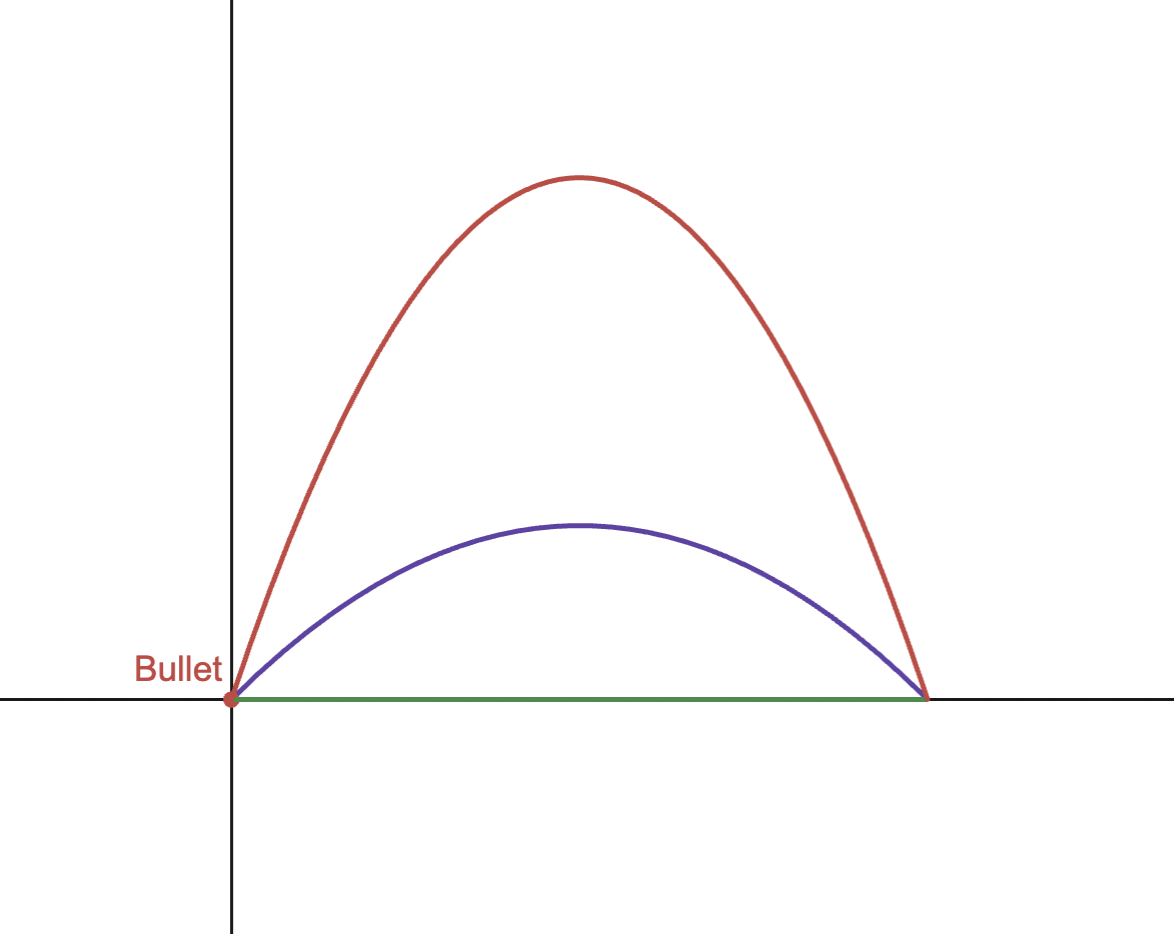
\includegraphics[width=0.5\linewidth]{picture/GRW1-1.png}
    \caption{A bullet and a baseball}
    \label{fig:5.1.1}
\end{figure}

This is because they are tracing out a \textbf{geodesic in spacetime}.They are both going the shortest \textit{distance} between the two points. 

Now with this knowledge, we assert that the gravitational mass and the inertial mass of an object is the same thing. Because according to the geodesic theory, the path that satisfy Newton's second law is precisely the path of the geodesic. 

Imagine an object sitting stationary on the earth surface, we would think of it as the normal force canceling the gravitational force. But in GR, the \textit{only} real force acting on the object is just the normal force that is holding it still. And we are just resisting the acceleration. Therefore \textit{weight} as measured by a scale is not real. And gravity is a very real thing. 

Einstein defined an equation that describes the curvature of spacetime near a certain flow of mass and energy. It is called the \textbf{Einstein Equation}, defined as follows
\begin{align}
\Lambda^{\mu\nu} = 8\pi GT^{\mu\nu}
\end{align}
Here, $\Lambda^{\mu\nu}$ is a $4\times4$ tensor that describes spacetime, and $T^{\mu\nu}$ is a $4\times4$ tensor that describes the distribution of the flow of mass and energy. The function of this equation can be condensed into a simple sentence said by physicist \textit{John Archibald Wheeler}
\begin{align}
\textit{Spacetime tells matter how to move; matter tells spacetime how to curve.}
\end{align}
And the study of general relativity is something that systematically investigate this behavior. 


\section{Special Relativity Review}
The definition of a spacetime interval can be seen earlier in this note so redundant information is not articulated. 

If we define the \textbf{proper time} between 2 events as $\boldsymbol\Delta\boldsymbol\tau$, then we can define it as follows
\begin{align}
\boldsymbol\Delta\boldsymbol\tau = \int_{\Delta t }\sqrt{-ds^2} =\int_{\Delta t} \frac{1}{\gamma}\,dt
\end{align}



\section{Four Vectors}
Introductory level for four vectors has been covered previously. We define \textbf{4 velocity} as follows
\begin{align}
d\mathbf{s} = \begin{bmatrix}
    dt\\dx\\dy\\dz
\end{bmatrix}
\end{align}
And the 4 velocity is defined as
\begin{align}
\mathbf{u}\equiv \frac{d\mathbf{s}}{d\tau}=
\begin{bmatrix}
    u_t\\u_x\\u_y\\u_z
\end{bmatrix}
\end{align}
We can also convert the differentials between frame with Lorenz Transform.

\begin{align}
\begin{bmatrix}
dt' \\
dx' \\
dy' \\
dz'
\end{bmatrix}
=
\begin{bmatrix}
\gamma & -\gamma\beta & 0 & 0 \\
-\gamma\beta & \gamma & 0 & 0 \\
0 & 0 & 1 & 0 \\
0 & 0 & 0 & 1
\end{bmatrix}
\begin{bmatrix}
dt \\
dx \\
dy \\
dz
\end{bmatrix}
\end{align}
And consequently
\begin{align}
\mathbf{u}' = \begin{bmatrix}
\gamma & -\gamma\beta & 0 & 0 \\
-\gamma\beta & \gamma & 0 & 0 \\
0 & 0 & 1 & 0 \\
0 & 0 & 0 & 1
\end{bmatrix}\mathbf{u}
\end{align}
Also, when we are taking the magnitude of a 4 vector, do not forget that we are dealing with Minkowski space. So when we are defining dot product in this space, what we are really doing is as follows
\begin{align}
\mathbf{u}\cdot \mathbf{v} = \mathbf{u}^T\eta\mathbf{v}
\end{align}
Where $\eta$ is the Minkowski measure, and is defined as
\begin{align}
\eta = \begin{bmatrix}
    -1&0&0&0\\
    0&1&0&0\\
    0&0&1&0\\
    0&0&0&1
\end{bmatrix}
\end{align}
this is also true for differentials
\begin{align}
d\mathbf{s}\cdot d\mathbf{s} = d\mathbf{s}^T\eta d\mathbf{s}
\end{align}
And important result to know is that, for any 4 velocity, the magnitude is always
\begin{align}
\mathbf{u}\cdot \mathbf{u} = -1
\end{align}
We can prove this easily. For any object moving with velocity $v$ in a given frame, the components of our 4 velocity is always
\begin{align}
\mathbf{u}=\begin{bmatrix}
    \gamma\\ \gamma u_x \\ \gamma u_y \\\gamma u_z 
\end{bmatrix}
\end{align}
And if we would carry out its dot product, we get the power result of $5.1$. And if we would look at our definition for 4 velocity
\begin{align}
\mathbf{u} = \dydx{\mathbf{s}}{\tau}
\end{align}
We also know from BOX 2.7 that
\begin{align}
d\tau = \frac{dt}{\gamma}
\end{align}
Therefore we can convert 4 velocity to ordinary velocity.
\begin{align}
\mathbf{u}= 
\begin{bmatrix}
u^t \\
u^x \\
u^y \\
u^z
\end{bmatrix}
=
\begin{bmatrix}
\frac{dt}{dt\sqrt{1 - v^2}} \\
\frac{dx}{dt\sqrt{1 - v^2}} \\
\frac{dy}{dt\sqrt{1 - v^2}} \\
\frac{dz}{dt\sqrt{1 - v^2}}
\end{bmatrix}
=
\begin{bmatrix}
\frac{1}{\sqrt{1 - v^2}} \\
\frac{v_x}{\sqrt{1 - v^2}} \\
\frac{v_y}{\sqrt{1 - v^2}} \\
\frac{v_z}{\sqrt{1 - v^2}}
\end{bmatrix}
\end{align}
The conversion between ordinary velocity and 4 velocity is then written as
\begin{align}
\mathbf{v} = \frac{1}{u_t}\mathbf{u}_{xyz}
\end{align}
Here $\mathbf{u}_{xyz}$ just means the 4 velocity without the time component. An object at rest will have 4 velocity of $u_t = 1$ and everything else $0$. When an object is moving slowly compare to the speed of light, we can in fact just approximate the 4 velocity with ordinary velocity.
\begin{align}
\mathbf{u} = 
\begin{bmatrix}
u^t \\
u^x \\
u^y \\
u^z
\end{bmatrix}
\approx
\begin{bmatrix}
1 \\
v_x \\
v_y \\
v_z
\end{bmatrix}
\quad \text{when } v \ll 1
\end{align}
With this newly defined 4 velocity, we can define our \textbf{4 momentum}. As a side note, even in relativity, we would consider mass to be frame-independent. 
\begin{align}
\mathbf{p} = m\mathbf{u} &\implies 
\begin{bmatrix}
P^t \\
P^x \\
P^y \\
P^z
\end{bmatrix}
=
\begin{bmatrix}
mu^t \\
mu^x \\
mu^y \\
mu^z
\end{bmatrix}
=
\begin{bmatrix}
\frac{m}{\sqrt{1 - v^2}} \\
\frac{mv_x}{\sqrt{1 - v^2}} \\
\frac{mv_y}{\sqrt{1 - v^2}} \\
\frac{mv_z}{\sqrt{1 - v^2}}
\end{bmatrix}
\end{align}
Since this is a linear relationship with the 4 velocity, we can simply transform the momentum accordingly with Lorenz transform. And when you use the dot product to obtain its magnitude, do not forget to include the Minkowski measure as well. Consider $5.1$, we have another powerful result
\begin{align}
\mathbf{p}\cdot\mathbf{p} = m^2(\mathbf{u}\cdot \mathbf{u}) = -m^2
\end{align}
This shows that 4 momentum is always constant and frame independent. And we have arrived at \textbf{Conservation of 4 momentum}. Also, with our previously established approximation with ordinary velocity, we can show that with sufficiently slow speed, we just have our regular momentum.
\begin{align}
\mathbf{p} \approx m\mathbf{v}
\end{align}
Which is consistent with our classical observations. And 4 momentum tells us that Newtonian momentum is in fact not conserved across reference frames. What is really conserved is 4 momentum. Let us go one step further and define \textbf{Relativistic Momentum and Energy}.
\begin{align}
\mathbf{p}_R = \mathbf{p}_{xyz} 
\end{align}
We would simply take out the $t$ component of our 4 momentum and call it our relativistic momentum. What do we do with the time component? We call it Relativistic energy.
\begin{align}
E_R = p_t
\end{align}
And we have arrived at a new result
\begin{align}
m^2 = E^2 - \mathbf{p}_R^2
\end{align}
From here on, we would simply use $\mathbf{p}$ to indicate relativistic momentum. More specifically, we define the relativistic energy of an object to be
\begin{align}
E = m + K
\end{align}
And 
\begin{align}
K = m\paren{\frac{1}{\sqrt{1-v^2}}-1}
\end{align}
With these information, we can see that the four momentum of light is purely kinetic since it has no mass. 

The energy in a given observer's frame is defined by
\begin{align}
-\mathbf{p}\cdot \mathbf{u}_{o} = p_t = E
\end{align}
We have found that regardless of the observer and frame where we would have different $\mathbf{p}$ and $\mathbf{u}_o$, energy calculated from this method is \textbf{always the same}. This is a very important result and we will find this helpful in future calculations. 


\section{Index Notation}
We will write Lorenz transform as
\begin{align}
\Lambda = \begin{bmatrix}
    \Lambda^{t}_{t}&\Lambda^{t}_{x}&\Lambda^{t}_{y}&\Lambda^{t}_{z}\\
    \Lambda^{x}_{t}&\Lambda^{x}_{x}&\Lambda^{x}_{y}&\Lambda^{x}_{z}\\
    \Lambda^{y}_{t}&\Lambda^{y}_{x}&\Lambda^{y}_{y}&\Lambda^{y}_z{}\\
    \Lambda^{z}_{t}&\Lambda^{z}_{x}&\Lambda^{z}_{y}&\Lambda^{z}_{z}
\end{bmatrix}
\end{align}
And the inverse as everything $\Lambda$ but replaced with $\paren{\Lambda^{-1}}$ We have only looked at very special case where the non-zero term in the transformation is expressed as
\begin{align}
&\etensor{\Lambda}{t}{t} = \etensor{\Lambda}{x}{x}=\gamma \\
&\etensor{\Lambda}{x}{t} = \etensor{\Lambda}{t}{x}= -\gamma\beta\\
&\etensor{\Lambda}{y}{y} =\etensor{\Lambda}{z}{z} = 1
\end{align}
But for a more generalized orientation of movement, we need to legitimately define the entire thing. These notation is extremely painful to write, let along doing them in \LaTeX. And imagine doing this all the time in relativity. Therefore, we need a much more simplified tool to represent all these stuff. Let me introduce you, the \textbf{Abstract Indices}.
\begin{align}
A^{\mu} \in \{A^{t}, A^{x},A^{y},A^{z}\}
\end{align}
\begin{align}
A_{\nu} \in \{A_{t},A_{x},A_{y},A_{z} \}
\end{align}
The \textbf{superscript as row} in the matrix, and \textbf{subscript as column} in the matrix. Now, we can rest assure that no more \textit{begin\{bmatrix\}} nonsense. 
Now, if we have a for vector $\mathbf{a}$, and we would like to apply Lorenz transformation on it, like below
\begin{align}
\begin{bmatrix}
    A'^t \\
    A'^x \\
    A'^y \\
    A'^z
\end{bmatrix}
=
\begin{bmatrix}
    \Lambda^t_t & \Lambda^t_x & \Lambda^t_y & \Lambda^t_z \\
    \Lambda^x_t & \Lambda^x_x & \Lambda^x_y & \Lambda^x_z \\
    \Lambda^y_t & \Lambda^y_x & \Lambda^y_y & \Lambda^y_z \\
    \Lambda^z_t & \Lambda^z_x & \Lambda^z_y & \Lambda^z_z
\end{bmatrix}
\begin{bmatrix}
    A^t \\
    A^x \\
    A^y \\
    A^z
\end{bmatrix}
\end{align}
We can actually just write it as
\begin{align}
A'^{\mu} = \sum_{\nu=t,x,y,z} \etensor{\Lambda}{\mu}{\nu}A^\nu
\end{align}
The summation sign still feels annoying right? Why not get rid of it from the get go. Welcome, \textbf{Einstein Summation Convention}! Dude is so smart he figured out shortcut to do all these tensors. What a legend. This convention states that, without further explanation, and if $\mu,\nu$ appeared exactly once precisely at the superscript and subscript, we assume it is a summation. defined above. So, we can simply rewrite the transformation matrix as
\begin{align}
A'^{\mu} = \etensor{\Lambda}{\mu}{\nu}A^\nu
\end{align}
Think of it this way, you have a column vector with 4 dimensions, it means this is a $4\times 1$ tensor. And you have 4 rows, each of only 1 element. Now, you have a matrix $\Lambda$, a $4\times 4$ tensor. You would like to perform a matrix multiplication. What happens is that you multiply each element in a row, that is, if you have a $m\times n$ matrix, you fix $m$ and start counting $n$, or each element in the row, then multiply it by each element in the column of the column vector, this return you the element in the $m$ position in our new column vector.
Now, we define something new, the \textbf{Metric Tensor}. Our Minkowski metric $\eta$ can be written as
\begin{align}
\eta_{\mu\nu}=
\begin{bmatrix}
    \eta_{tt} & \eta_{tx} & \eta_{ty} & \eta_{tz} \\
    \eta_{xt} & \eta_{xx} & \eta_{xy} & \eta_{xz} \\
    \eta_{yt} & \eta_{yx} & \eta_{yy} & \eta_{yz} \\
    \eta_{zt} & \eta_{zx} & \eta_{zy} & \eta_{zz}
\end{bmatrix}
\equiv
\begin{bmatrix}
    -1 & 0 & 0 & 0 \\
     0 & 1 & 0 & 0 \\
     0 & 0 & 1 & 0 \\
     0 & 0 & 0 & 1
\end{bmatrix}
\end{align}
Where $\mu$ is the row, and $\nu$ is the column. Both in subscript, and a little different from before. With this in mind, we can now rewrite the metric equation as
\begin{align}
ds^2 = \eta_{\mu\nu}dx^{\mu}dx^{\nu}
\end{align}
Think of $dx^{\mu}dx^{\nu}$ as going through a permutation of $(t,x,y,z)\times(t,x,y,z)$. This will give us a complete metric that properly describes spacetime. In our flat Minkowski space, this is simply written as
\begin{align}
ds^2 &= \eta_{tt} dt^2 + \eta_{xx} dx^2 + \eta_{yy} dy^2 + \eta_{zz} dz^2 \nonumber \\
     &= -dt^2 + dx^2 + dy^2 + dz^2
\end{align}

We can similarly write the dot product of two four-vectors as

\begin{align}
\mathbf{A} \cdot \mathbf{B} = \eta_{\mu \nu} A^\mu B^\nu
\end{align}

and the squared magnitude of a four-vector as

\begin{align}
A^2 = \mathbf{A} \cdot \mathbf{A} = \eta_{\mu \nu} A^\mu A^\nu. 
\end{align}
We seem to be making stuff more complicated, but behold. This will come in clutch in future studies. Now, we would also need some help from the \textbf{Kronecker Delta} $\etensor{\delta}{\mu}{\nu}$. In case you are not familiar with this, it simply means
\[
\etensor{\delta}{\mu}{\nu} = \begin{cases}
    1 &\mu=\nu\\
    0 &\mu\neq\nu
\end{cases}
\]
If expanded, you may notice that it is just the identity matrix. Since we know that $\Lambda^{-1}\Lambda = I$, we can also write it as
\[
\etensor{\paren{\Lambda^{-1}}}{\mu}{\alpha}\etensor{\Lambda}{\alpha}{\nu} = \etensor{\delta}{\mu}{\nu}
\]
The sums are implicit over all possible value of $\alpha$. Another useful property of this notation is that
\[
\etensor{\delta}{\mu}{\nu}A^{\nu } = AA^{\mu}
\]
\[
\etensor{\delta}{\mu}{\alpha}\eta_{\mu\nu} = \eta{\alpha\nu}
\]
We can also write the \textbf{Electromagnetic Field Tensor} as
\[
\begin{bmatrix}
F^{tt} & F^{tx} & F^{ty} & F^{tz} \\
F^{xt} & F^{xx} & F^{xy} & F^{xz} \\
F^{yt} & F^{yx} & F^{yy} & F^{yz} \\
F^{zt} & F^{zx} & F^{zy} & F^{zz}
\end{bmatrix}
=
\begin{bmatrix}
0 & E_x & E_y & E_z \\
-E_x & 0 & B_z & -B_y \\
-E_y & -B_z & 0 & B_x \\
-E_z & B_y & -B_x & 0
\end{bmatrix}
\]  
And we can write the relativistic version of Lorentz Force Law
\[
\frac{\text{d}p^\mu}{\text{d}\tau}=qF^{\mu\nu}\eta_{\nu\alpha}u^{\alpha}
\]
And we can write the Gauss's law and the Ampere-Maxwell relation become the single equation
\[
\pypx{F^{\mu\nu}}{x^\nu} = 4\pi k J^\mu = \frac{J^{\mu}}{\varepsilon_0}
\]
Where $k = \frac{1}{4\pi\varepsilon_0}$, and $J^t = \rho,J^x=\rho v_x$ and etc. And if a subscript or superscript appeared throughout an equation for multiple times, we call it a \textbf{Free index} since we can assign a certain value to it to investigate the value we are interested. 
And if you are not sure if working with stuff with abstract indices is legal or not, just write the entire tensor out to check, no big deal. 

We wrap this up by some nice identities
\[
\eta_{\alpha\beta}=\eta_{\mu\nu}\etensor{\Lambda}{\mu}{\alpha}\etensor{\Lambda}{\nu}{\beta}
\]
\[
\eta_{\alpha\beta}=\eta_{\mu\nu}\etensor{\paren{\Lambda^{-1}}}{\mu}{\alpha}\etensor{\paren{\Lambda^{-1}}}{\nu}{\beta}
\]
We also have a useful result for a given 4 vector $\mathbf{a}$
\[
\dydx{}{\tau}\mathbf{A}^2 = 2\eta_{\mu\nu}A^{\mu}\dydx{A^{\nu}}{\tau}
\]
And for electromagnetic force, since $F^{\mu\nu} = -F^{\nu\mu}$, we have
\[
F^{\mu\nu}\eta_{\mu\alpha}\eta_{\nu\beta}u^{\alpha}u^{\beta} = 0
\]
Regardless of what the four velocity $\mathbf{u}$ is, since we all know it has constant magnitude. 

\section{}

\chapter{Spacetime and Geometry - Sean Carroll}
\section{Manifold}
\subsection{Equivalence Principles}
We can define some universal properties across gravitational interaction. It is primarily characterized in 3 different principles.
\subsubsection{Weak Equivalence Principle}
The \textbf{WEP} states that the inertial mass and gravitational mass of any object are equal. This basically means that the $m$ in Newton's second law and the Newton's law of gravity are the same.

A more elegant way of stating this would be: \textit{The motion of free falling particles are the same in a gravitational field and a uniformly accelerated frame, in small enough regions of spacetime.}

\subsubsection{EInstein Equivalence Principle}
The \textbf{EEP} states that \textit{in any small enough regions of spacetime, the laws of physics reduce to special relativity, and is impossible to detect the existence of a gravitational field by means of local experiments.}

This is the principle that we build our inertial reference frame on. 

\subsection{Vectors}
We define a vector as follows
\[
\dydx{}{\lambda} = \dydx{x^\mu}{\lambda}\pypx{}{x^\mu}
\]
Where $x^\mu$ encodes certain information about the manifold or basis we are using. And to swap a base, we can use chain rule, and obtain
\[
\pypx{}{x^{\mu'}} = \pypx{x^{\mu}}{x^{\mu'}}\pypx{}{x^{\mu}}
\]
We want to define a vector field as follows
\[
\sqbkt{X,Y}^\mu = X^{\lambda}\partial_{\lambda}Y^{\mu}-Y^{\lambda}\partial_{\lambda}X^{\mu}
\]













\end{document}
